\documentclass[12pt,a4paper]{report}
\usepackage[utf8]{inputenc}
\usepackage{amsmath,amssymb}
\usepackage{graphicx}
\usepackage[margin=.75in]{geometry}
\usepackage{xcolor}
\usepackage{tikz}
\usepackage{tikz-cd}
\usepackage{algpseudocode}
\usepackage{booktabs}
\usepackage{enumitem}
\usepackage{algorithm}
\usepackage{natbib}
\usepackage{makecell}
\usepackage{amsthm}
% \usepackage{natbib} % Duplicate removed
% \usepackage{xcolor}  % Duplicate removed
\usepackage[colorlinks=true, citecolor=black]{hyperref}

% Redefine \citep to be small, italic, and blue
\renewcommand{\citep}[1]{\textit{\scriptsize{(\cite{#1})}}}

\newtheorem{definition}{Definition}[section]
\newtheorem{theorem}{Theorem}[section]

\usetikzlibrary{shapes,arrows,positioning,fit,backgrounds}
\usetikzlibrary{calc}
\hypersetup{
	colorlinks=true,
	linkcolor=blue,
	filecolor=magenta,
	urlcolor=cyan,
	pdftitle={Open AMI: Compliant Machine Learning and Automation Framework Rev.1},
	pdfauthor={Independent AI Labs}
}
% Define consistent terminology for pillars to ensure clarity
% Using bold for emphasis when introducing/referring to the concept
\newcommand{\Compliance}{\textbf{Compliance}}
\newcommand{\Integrity}{\textbf{Integrity}}
\newcommand{\Abstraction}{\textbf{Abstraction}}
\newcommand{\Dynamics}{\textbf{Dynamics}}
% Alternative command for less emphasis in running text if needed
\newcommand{\compliance}{compliance}
\newcommand{\integrity}{integrity}
\newcommand{\abstraction}{abstraction}
\newcommand{\dynamics}{dynamics}
\title{{\LARGE Open AMI: \LARGE Compliant Machine Learning and Automation\\\textit{\normalsize{Rev.1}}}}
\author{Vladislav Donchev\\Open AMI (Advanced Machine Intelligence), Independent AI Labs\\ \\\normalsize{\href{mailto:v.donchev@independentailabs.com}{v.donchev@independentailabs.com}}}
\date{May 26, 2025}
\begin{document}
	\begin{titlepage}
		\maketitle
		\vspace{2cm}
		\begin{abstract}
			The increasing sophistication and autonomy of Artificial Intelligence (AI) and Machine Learning (ML) systems necessitate rigorous approaches to ensure their trustworthiness \citep{Li2021}. However, prevailing AI/ML development pipelines often lack integrated mechanisms for achieving verifiable \textbf{Compliance} (encompassing safety, ethics, and legal adherence), maintaining data and computational \textbf{Integrity} \citep{Balan2025}, managing complexity through transparent \textbf{Abstraction} \citep{Spoczynski2025}, or governing adaptive system \textbf{Dynamics} robustly \citep{AdditionalCitationRef2, Hinder2024}. These deficiencies, recognized as critical gaps in trustworthy AI \citep{AdditionalCitationRef1}, are frequently addressed through fragmented or manual processes \citep{AdditionalCitationRef2} and are exacerbated in emerging agentic systems reliant on complex compositions with potential reliability and security vulnerabilities \citep{Schneider2024, Narajala2025}.
			
			This paper introduces \textbf{Open AMI}, a unified theoretical and architectural framework designed to embed trustworthiness throughout the ML and solution development lifecycle. Open AMI provides a structured environment integrating process theory, cognitive analogues, secure distributed computation, and adaptive control principles, governed by its four core pillars: \Compliance, \Integrity, \Abstraction, and \Dynamics.
			
			The framework's main design goal is to build on existing standards (e.g. ISO/IEC), frameworks (such as NIST CSF and RMF) and protocols (Google A2A \citep{A2A_README}, etc.), enabling advanced agentic AI, ML and workflow automation in a demonstrably compliant and verifiable manner.
			
			\vspace{0.5cm} % Adjusted spacing slightly
			\textbf{Keywords:} Artificial Intelligence, Machine Learning, Advanced Machine Intelligence, AMI, AI Compliance, AI Safety, Trustworthy AI, Cognitive Architectures, Secure Distributed Systems, System Dynamics, Abstraction Management, Data Integrity, Verifiable Computation, Continuous Learning, Federated Learning, Reinforcement Learning, Model Interoperability, Physical Grounding, Open AMI, Agentic AI
		\end{abstract}
		\vfill
		\begin{center}
			\textbf{Note:} Experimental data, documentation, and code libraries enabling the implementation of Open AMI systems will be published on \href{https://www.independentailabs.com}{www.independentailabs.com} and \href{https://github.com/Independent-AI-Labs/OpenAMI}{GitHub}.
			\paragraph{}
			\href{https://github.com/Independent-AI-Labs/OpenAMI}{https://github.com/Independent-AI-Labs/OpenAMI}
			\vspace{0.5cm}
			\paragraph{}
			This is a DRAFT paper intended for peer review.
		\end{center}
	\end{titlepage}
	
		\chapter{Advancing Toward Trustworthy AI Systems}
	\label{ch:introduction}
	\section{Introduction}
	The rapid advancement of artificial intelligence (AI) and machine learning (ML) systems has already transformed numerous domains. As these systems become increasingly sophisticated, autonomous, and integrated into critical aspects of society, \textit{ensuring their trustworthiness becomes paramount}.
	
	Modern ML development pipelines (often termed MLOps), while powerful, frequently lack \textbf{integrated} mechanisms for continuously verifying adherence to compliance standards, guaranteeing computational integrity, navigating system complexity across levels of abstraction, or managing the dynamics of ongoing learning and adaptation in a principled manner. This gap becomes particularly acute as we move towards more autonomous, agentic systems \citep{AgenticLandscape_Ref19} or explore capabilities associated with Artificial General Intelligence (AGI), where failure modes like reward hacking or unsafe exploration become more severe and difficult to control \citep{AdditionalCitationRef3, AdditionalCitationRef27Modern}. Furthermore, the increasing reliance on composing large models with external tools—a common pattern in current agentic AI exemplified by systems for task orchestration, such as Perplexity's research engine \citep{Perplexity2024DeepResearch}, introduces new failure modes, such as inter-agent misalignment or error propagation, and complicates verification \citep{AdditionalCitationRef7}.
	
	This paper introduces \textbf{Open AMI (Advanced Machine Intelligence)}—a comprehensive framework designed to address these challenges. Open AMI provides an integrated theoretical foundation and architectural blueprint for developing, deploying, and managing AI/ML systems that are secure, compliant, adaptive, and capable of continuous, grounded learning. Unlike approaches that treat trustworthiness as an add-on or focus narrowly on model performance or specific agent capabilities, Open AMI embeds these principles throughout the entire AI/ML lifecycle, from data governance and model training to deployment, operation, and ongoing adaptation.
	
	\subsection{Motivation: Limitations of Current AI/ML Practices}
	\label{sec:1-1}
	While current AI/ML techniques, particularly deep learning and large language models (LLMs), have achieved remarkable success across diverse domains \citep{AdditionalCitationRef8, Xie2025LLMAgentsSurvey}, their application reveals significant limitations concerning trustworthiness and manageability \citep{Bandam2025, AdditionalCitationRef33}:
	
	\begin{itemize}[leftmargin=*]
		\item \textbf{Compliance Gaps in ML Lifecycles:} Ensuring adherence to ethical guidelines, legal requirements (e.g., data privacy, fairness regulations), and safety constraints throughout the data collection, training, deployment, and update phases of ML models is often handled through manual audits or via disconnected tools \citep{Bhardwaj2024AIGovMLOps}. This lack of integration makes continuous verification of compliance difficult and prone to error, as risks can evolve dynamically \citep{AdditionalCitationRef12}, despite explicit regulatory mandates for AI conformity assessments (e.g., EU AI Act Art. 43 \citep{EUAIAct2024}) \citep{Navigating_AI_Conformity_2025, AgenticLandscape_Ref26}.
		\item \textbf{Integrity Challenges in Computation and Data:} Verifying the integrity of training data, ensuring the correctness and reproducibility of complex training processes (often termed the ML pipeline integrity problem), and guaranteeing the reliable execution of deployed models (especially in distributed or composed systems) remain significant hurdles. The provenance of data and models is often poorly tracked \citep{AgenticLandscape_Ref25}, hindering accountability and verification, though techniques like Proof-of-Learning (PoL) aim to address this \citep{Jia2021ProofOfLearning}.
		\item \textbf{Reliability of Complex Reasoning/Computation:} The "LLM + Tools" paradigm \citep{AgenticLandscape_Ref49}, while extending capabilities, outsources complex computation (e.g., via code generation/execution). Studies show LLM-generated code often contains significantly more security vulnerabilities than human code \citep{AdditionalCitationRef14}, introducing substantial reliability and security concerns. Ensuring the integrity and correctness of these complex, often brittle, reasoning chains is difficult, as LLM reasoning can be inconsistent or prone to hallucination \citep{AgenticLandscape_Ref86}.
		\item \textbf{Opacity and Abstraction Barriers:} Modern ML models, especially deep neural networks and LLMs, are notoriously opaque ("black boxes") \citep{AdditionalCitationRef42}. Understanding their internal representations, debugging failures, or explaining decisions requires specialized techniques that are often insufficient. Managing complexity requires navigating different levels of abstraction, from low-level weights to high-level emergent behaviors, which current tools poorly support \citep{AgenticLandscape_Ref25}. Notable contributions to mechanistic interpretability, such as feature decomposition via dictionary learning \citep{AdditionalCitationRef15}, aim to decompose model internals into understandable components \citep{Anthropic_Decompose_2023}.
		\item \textbf{Managing Learning Dynamics and Adaptation:} Systems designed for continuous learning or adaptation (e.g., via online learning or reinforcement learning) face challenges in ensuring stability, preventing catastrophic forgetting \citep{Wang2024ContinualLearningSurvey, AdditionalCitationRef24}, and managing the exploration/exploitation trade-off safely, a challenge addressed in safe reinforcement learning research \citep{AdditionalCitationRef16}. Controlling these adaptive dynamics while maintaining compliance and integrity is non-trivial, especially given the fragility of models to distribution shifts \citep{AdditionalCitationRef17, AdditionalCitationRef18}.
		\item \textbf{Brittleness and Lack of Grounding:} Models often fail unexpectedly when encountering out-of-distribution data or slight environmental perturbations. Many systems lack grounding in the physical or causal structure of the world, relying instead on statistical correlations, which limits their robustness and common-sense reasoning capabilities, a limitation highlighted in AI commonsense research \citep{AdditionalCitationRef19, Physics-InspiredReasoning_Ref34}. Simulation-based learning is a key strategy to address this \citep{Li2025DigitalTwins}.
		\item \textbf{Interoperability and Composition Issues:} Integrating diverse ML models or AI components developed using different tools or paradigms is often difficult due to mismatched assumptions and interfaces \citep{AdditionalCitationRef20}, hindering the creation of complex, multi-component systems that might leverage collaborative learning or specialized capabilities \citep{AgenticLandscape_Ref43}. Secure and verifiable composition remains a challenge, requiring standardized protocols that provide stronger guarantees than basic agent communication primitives to handle semantic inconsistencies and ensure trust \citep{AdditionalCitationRef21}.
	\end{itemize}
	
	These limitations underscore the need for a new generation of frameworks that build trustworthiness in from the start. Open AMI aims to provide such a foundation, enabling the development of AI/ML systems where learning, adaptation, and complex computation occur within a secure, compliant, verifiable, and manageable environment.
	
	\subsection{The Open AMI Unified Architecture}
	\begin{figure}[ht]
		\centering
		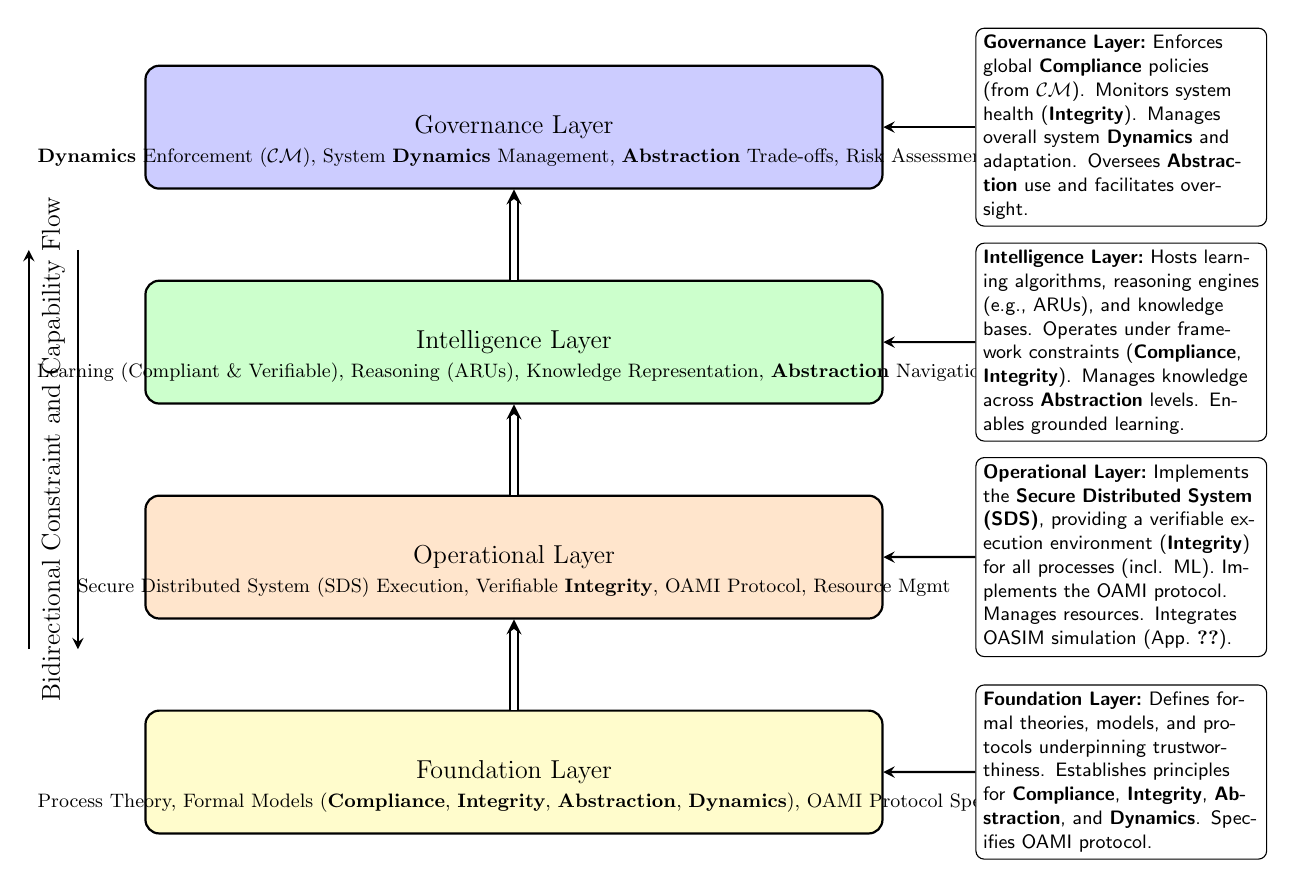
\begin{tikzpicture}[
			node distance=1.5cm,
			auto,
			scale=0.78,
			transform shape,
			layer/.style={
				rectangle,
				draw,
				thick,
				rounded corners=5pt,
				minimum width=12cm,
				minimum height=2cm,
				text width=11.5cm,
				align=center,
				font=\bfseries
			},
			sublayer/.style={
				font=\small,
				align=center
			},
			sidebox/.style={
				rectangle,
				draw,
				fill=white,
				text width=4.5cm,
				align=left,
				font=\small\sffamily,
				rounded corners=3pt,
			},
			arrow/.style={-stealth, thick}
			]
			% The four architecture layers with distinct colors
			\node[layer, fill=blue!20, font=\large] (governance) at (0,0) {Governance Layer};
			\node[sublayer] at (0,-0.5) {\Dynamics\ Enforcement ($\mathcal{CM}$), System \Dynamics\ Management, \Abstraction\ Trade-offs, Risk Assessment};
			\node[layer, fill=green!20, font=\large] (intelligence) at (0,-3.5) {Intelligence Layer};
			\node[sublayer] at (0,-4.0) {Learning (Compliant \& Verifiable), Reasoning (ARUs), Knowledge Representation, \Abstraction\ Navigation};
			\node[layer, fill=orange!20, font=\large] (operational) at (0,-7) {Operational Layer};
			\node[sublayer] at (0,-7.5) {Secure Distributed System (SDS) Execution, Verifiable \Integrity, OAMI Protocol, Resource Mgmt};
			\node[layer, fill=yellow!20, font=\large] (foundation) at (0,-10.5) {Foundation Layer};
			\node[sublayer] at (0,-11.0) {Process Theory, Formal Models (\Compliance, \Integrity, \Abstraction, \Dynamics), OAMI Protocol Spec};
			% Bidirectional arrows connecting the layers (adjusted spacing)
			\draw[arrow, double, double distance=2pt] (foundation.north) -- (operational.south);
			\draw[arrow, double, double distance=2pt] (operational.north) -- (intelligence.south);
			\draw[arrow, double, double distance=2pt] (intelligence.north) -- (governance.south);
			% Side boxes with explanatory text on the right side (adjusted positions)
			\node[sidebox, right=1.5cm of foundation] (foundation_text) {
				\textbf{Foundation Layer:}\
				Defines formal theories, models, and protocols underpinning trustworthiness. Establishes principles for \Compliance, \Integrity, \Abstraction, and \Dynamics. Specifies OAMI protocol.
			};
			\draw[arrow] (foundation_text.west) -- (foundation.east);
			\node[sidebox, right=1.5cm of operational] (operational_text) {
				\textbf{Operational Layer:}\
				Implements the \textbf{Secure Distributed System (SDS)}, providing a verifiable execution environment (\Integrity) for all processes (incl. ML). Implements the OAMI protocol. Manages resources. Integrates OASIM simulation (App.~\ref{app:simulation_subsystem}).
			};
			\draw[arrow] (operational_text.west) -- (operational.east);
			\node[sidebox, right=1.5cm of intelligence] (intelligence_text) {
				\textbf{Intelligence Layer:}\
				Hosts learning algorithms, reasoning engines (e.g., ARUs), and knowledge bases. Operates under framework constraints (\Compliance, \Integrity). Manages knowledge across \Abstraction\ levels. Enables grounded learning.
			};
			\draw[arrow] (intelligence_text.west) -- (intelligence.east);
			\node[sidebox, right=1.5cm of governance] (governance_text) {
				\textbf{Governance Layer:}\
				Enforces global \Compliance\ policies (from $\mathcal{CM}$). Monitors system health (\Integrity). Manages overall system \Dynamics\ and adaptation. Oversees \Abstraction\ use and facilitates oversight.
			};
			\draw[arrow] (governance_text.west) -- (governance.east);
			% Bidirectional flow indication (adjusted position)
			\node[font=\large, rotate=90] at (-7.5,-5.25) {Bidirectional Constraint and Capability Flow};
			\draw[-stealth, thick] (-7.9,-8.5) -- (-7.9,-2);
			\draw[-stealth, thick] (-7.1,-2) -- (-7.1,-8.5);
		\end{tikzpicture}
		\caption[Open AMI Unified Architecture]{The Open AMI Unified Architecture. Four interconnected layers provide a structured environment for developing, deploying, and managing trustworthy AI/ML systems. Constraints (such as \Compliance\ rules from the Compliance Manifest ($\mathcal{CM}$) and \Integrity\ requirements enforced by the SDS) flow down, while capabilities and status information flow up, ensuring cohesive operation across levels of \Abstraction\ and robust management of system \Dynamics.}
		\label{fig:open_ami_architecture}
	\end{figure}
	
	As illustrated in Figure~\ref{fig:open_ami_architecture}, Open AMI integrates four interconnected layers:
	
	\begin{itemize}[leftmargin=*]
		\item \textbf{Foundation Layer}: Establishes the theoretical basis and formal definitions for the core pillars: \Compliance, \Integrity, \Abstraction, and system \Dynamics. Includes Process Theory, formal modeling techniques, and the OAMI communication protocol specification (Appendix~\ref{app:protocol_spec}).
		\item \textbf{Operational Layer}: Implements the \textbf{Secure Distributed System (SDS)}, detailed in Chapter~\ref{ch:secure_distributed_system}, providing the verifiable (\Integrity) execution environment. It handles secure communication (via the OAMI protocol, Appendix~\ref{app:protocol_spec}) and resource management for all system processes, including ML model training and inference. It can integrate simulation capabilities, such as the Open AMI Simulation Subsystem (OASIM), detailed in Appendix~\ref{app:simulation_subsystem}.
		\item \textbf{Intelligence Layer}: Hosts the core AI/ML capabilities, including learning algorithms (supervised, unsupervised, RL), reasoning engines (potentially structured as directories (graphs) of Atomic Reasoning Units or ARUs, see Chapter~\ref{ch:theoretical_framework}), knowledge representation systems, and mechanisms for navigating different levels of \Abstraction. All operations within this layer are subject to the constraints and verification mechanisms enforced by the framework, enabling continuous, grounded learning (details on ML in Chapter~\ref{ch:machine_learning}).
		\item \textbf{Governance Layer}: Oversees the entire system, enforcing global \Compliance\ policies derived from the Compliance Manifest ($\mathcal{CM}$, detailed in Chapter~\ref{ch:compliance}). Monitors system health and \Integrity\ status, manages overall system \Dynamics\ (e.g., adaptation rate, stability), mediates trade-offs involving \Abstraction, and handles risk assessment and response.
	\end{itemize}
	
	These layers interact bidirectionally, creating a closed loop where requirements for \Compliance\ and \Integrity\ shape AI/ML development and operation, while performance and status data inform governance and adaptation. This architecture enables the creation of AI systems where trustworthiness is an intrinsic property, not an external check.
	
	\subsection{Core Capabilities and Innovations}
	Open AMI provides a framework for building AI/ML systems with the following core capabilities, framed by its four pillars:
	
	\begin{enumerate}[leftmargin=*]
		\item \textbf{Secure Distributed Computation with Verifiable Integrity:} An operational layer (SDS) that guarantees data and computation \Integrity\ for both ML training, inference and general data processing across diverse infrastructures, potentially leveraging techniques like ZKPs \citep{Peng2025ZKMLSurvey} or PoL \citep{Jia2021ProofOfLearning}.
		\item \textbf{Compliant Machine Learning Lifecycle:} Tools and protocols (centered around the $\mathcal{CM}$) for defining and enforcing \Compliance\ rules (regarding data usage, fairness, safety, etc.) throughout data preparation, model training, validation, deployment, and monitoring, aligning with principles of AI conformity assessment \citep{Navigating_AI_Conformity_2025}.
		\item \textbf{Transparent and Manageable Models:} Mechanisms for representing models and their learned knowledge across multiple levels of \Abstraction, facilitating debugging, explanation, and oversight, drawing inspiration from interpretable AI (XAI) approaches including techniques providing multiple levels of abstraction \citep{AdditionalCitationRef22} or feature decomposition \citep{Anthropic_Decompose_2023}.
		\item \textbf{Robust Adaptive Learning and Dynamics Management:} Support for continuous learning paradigms (e.g., online learning, RL) within a framework that actively manages stability and adaptation rate (\Dynamics), ensuring ongoing \Compliance, addressing core challenges highlighted in continual learning research such as stability-plasticity trade-offs and catastrophic forgetting \citep{Wang2024ContinualLearningSurvey, AdditionalCitationRef24}.
		\item \textbf{Grounded Learning and Experimentation:} Integration with simulation capabilities (e.g., OASIM, Appendix~\ref{app:simulation_subsystem}) allowing models to learn from physically realistic interactions or test hypotheses in a safe, verifiable environment, consistent with sim-to-real strategies \citep{Josifovski_SCDA_2025, Li2025DigitalTwins}.
		\item \textbf{High-Integrity Reasoning:} Support for structured and potentially more reliable reasoning mechanisms (e.g., ARUs, physics-inspired computation explored in Chapter~\ref{ch:theoretical_framework}) operating with guaranteed computational \Integrity, offering an alternative to less verifiable composed systems \citep{Cao_PhyDRL_2024}.
		\item \textbf{Interoperable and Collaborative Systems: A standardized protocol (OAMI, Appendix~\ref{app:protocol_spec}) enabling secure and effective collaboration, data sharing, and even collaborative learning between diverse AI/ML components built within the framework, addressing the need for advanced protocols beyond basic agent communication to handle trust and semantics}.
	\end{enumerate}
	
	The key innovations of Open AMI include:
	\begin{itemize}[leftmargin=*]
		\item The deep integration of \Compliance, \Integrity, \Abstraction, and \Dynamics\ management as fundamental architectural principles governing the entire AI/ML lifecycle.
		\item A formal framework (Chapter~\ref{ch:theoretical_framework}) and operational layer (SDS, Chapter~\ref{ch:secure_distributed_system}) specifically designed to support the development and management of trustworthy, continuously learning AI systems, incorporating cryptographic verification methods where feasible \citep{Peng2025ZKMLSurvey, Jia2021ProofOfLearning}.
		\item Mechanisms enabling verifiable, grounded learning through integrated simulation and experimentation capabilities (OASIM, Appendix~\ref{app:simulation_subsystem}).
		\item A standardized protocol (OAMI, Appendix~\ref{app:protocol_spec}) promoting verifiable interoperability and collaboration between compliant AI/ML components.
		\item Exploration of structured reasoning and physics-inspired computation as pathways to more inherently reliable AI \citep{Cao_PhyDRL_2024}.
	\end{itemize}
	
	\subsection{Scope and Objectives}
	Open AMI aims to provide a comprehensive framework for developing AI and ML systems that:
	
	\begin{itemize}[leftmargin=*]
		\item Learn, reason, and adapt while maintaining verifiable guarantees regarding \Compliance.
		\item Operate securely with verifiable computational and data \Integrity\ across their lifecycle.
		\item Allow for transparent oversight and management through navigable layers of \Abstraction.
		\item Exhibit robust and stable adaptive \Dynamics.
		\item Can be grounded in physical reality through integrated simulation.
		\item Can interoperate and collaborate effectively and safely.
	\end{itemize}
	
	Limitations acknowledged:
	\begin{itemize}[leftmargin=*]
		\item Open AMI provides a \textbf{framework}, not off-the-shelf AGI or specific ML models. Domain-specific implementation is required.
		\item Realizing the full potential, especially for highly adaptive or physically grounded systems, depends on advances in underlying technologies (computation, simulation, ML algorithms).
		\item The framework does not resolve fundamental philosophical questions about intelligence or consciousness.
	\end{itemize}
	
	\subsection{Paper Structure}
	The remainder of this paper is organized as follows:
	
	\begin{itemize}[leftmargin=*]
		\item \textbf{Chapter II: Theoretical Framework} presents the foundational theories, integrating Process Theory, Cognitive Mapping analogues, and formal models for reasoning and learning, all framed by the principles of \Compliance, \Integrity, \Abstraction, and system \Dynamics. Contextualized within the current agentic AI landscape and supported by external research in cognitive science, interpretability, and verifiable computation.
		\item \textbf{Chapter III: Machine Learning Paradigms in Open AMI} details how various ML approaches (supervised, unsupervised, RL, continuous learning, federated learning) are implemented, managed, and verified within the Open AMI framework's constraints, drawing on research in trustworthy ML, continual learning, and secure computation.
		\item \textbf{Chapter IV: Secure Distributed System (SDS)} details the architecture and mechanisms of the Operational Layer, focusing on secure execution with verifiable \Integrity, implementing the OAMI protocol, and supporting compliant ML operations, informed by advances in cryptographic verification and secure distributed systems.
		\item \textbf{Chapter V: Compliance and Core Directives} explores the ethical, legal, and operational guidelines formalized in the Compliance Manifest ($\mathcal{CM}$), and the mechanisms within the Governance Layer for their enforcement and verification, referencing AI safety, ethics frameworks, and constrained learning research.
		\item \textbf{Appendix A: Open AMI (OAMI) Protocol Specification:} Details the secure interaction protocols enabling communication, task management, and knowledge sharing between OAMI components, extending concepts from agent communication standards.
		\item \textbf{Appendix B: Open AMI Simulation Subsystem (OASIM) Specification:} Outlines the integrated simulation capability for physical grounding, verification, and embodied agent support, emphasizing USD/Omniverse compatibility and referencing digital twin and sim-to-real research.
		\item \textbf{Appendix C: Open AMI Compliance Map:} Maps the Open AMI framework's principles, architecture, and components to key requirements of major AI governance, risk management, information security, and ethical standards.
		\item \textbf{Appendices D-N: Proof Sketches for Selected Theorems:} Provides high-level outlines for the proofs of theorems presented in the main text.
		\item \textbf{Chapter VI: Evaluation and Validation} (Work in Progress) will present theoretical analyses, simulations, and preliminary experimental results validating key aspects of the Open AMI framework.
		\item \textbf{Chapter VII: Applications and Case Studies} (Work in Progress) will demonstrate the application of Open AMI to specific AI/ML development scenarios.
		\item \textbf{Chapter VIII: Conclusion and Future Directions} (Work in Progress) will summarize contributions and outline future research, focusing on trustworthy adaptive learning and model interoperability.
		\item \textbf{Chapter IX: References} Consolidated bibliography.
	\end{itemize}
	
	By providing a structured, verifiable, and compliant environment for the entire AI/ML lifecycle, Open AMI aims to foster the development of advanced artificial intelligence that is not only powerful but also fundamentally trustworthy.
	
		\chapter{Theoretical Framework}
	\label{ch:theoretical_framework}
	
	\section{Introduction to the Open AMI Theoretical Framework}
	\label{sec:2-1}
	
	The Open AMI (Advanced Machine Intelligence) framework provides an integrated theoretical foundation for developing trustworthy Artificial Intelligence (AI) and Machine Learning (ML) systems capable of complex reasoning, adaptation, and continuous learning. This chapter outlines the formal theoretical underpinnings that enable Open AMI to guide the construction of systems that are not only capable but also secure, aligned, transparent, and robustly adaptive. The framework's foundations draw upon process theory, cognitive mapping analogues inspired by self-organizing knowledge networks \citep{Buehler2025AgenticGraphRef}, state-space modeling, structured reasoning units, and secure computation principles, demonstrating how these theories inform the practical architecture detailed in later chapters.
	
	\subsection{Positioning Within the AI Research Landscape}
	\label{sec:2-1-1}
	
	Open AMI draws from and extends multiple research traditions, aiming to address limitations observed in current advanced AI systems, particularly in the burgeoning field of \textbf{Agentic AI} \citep{AgenticLandscape_Ref19}, including agentic graph reasoning approaches \citep{Buehler2025AgenticGraphRef}. While the theoretical pursuit of Artificial General Intelligence (AGI) continues, facing significant open challenges \citep{AdditionalCitationRef27, AdditionalCitationRef27Modern}, the practical frontier features agentic systems leveraging Large Language Models (LLMs) augmented with planning, memory, and tool-using capabilities.
	
	The prevailing paradigm is often described as \textbf{"Reasoning LLMs + Tool Use"} \citep{Yang2025LLMAgentParadigms}. Systems built using frameworks like LangGraph \citep{AgenticLandscape_Ref106, AgenticLandscape_Ref19}, or specialized agents like Devin \citep{AgenticLandscape_Ref14} or OpenHands \citep{OpenHandsRef}, typically employ an LLM as a central reasoning engine that interacts with external tools (web search, code interpreters, APIs) to overcome intrinsic LLM limitations, such as knowledge cutoffs or poor calculation abilities \citep{AgenticLandscape_Ref86}. While effective for automating complex digital tasks (e.g., coding, research \citep{AdditionalCitationRef32, AgenticLandscape_Ref40}), this approach presents challenges:
	
	\begin{itemize}[noitemsep]
		\item \textbf{Reliability and Robustness Gaps:} LLM-driven reasoning can be brittle, prone to hallucinations, inconsistent \citep{AgenticLandscape_Ref86}, and produce "sensible yet wrong" answers \citep{AdditionalCitationRef33}. Delegating computation via generated code introduces further reliability and security risks, as AI-generated code often contains more vulnerabilities \citep{Physics-InspiredReasoning_Ref10, AdditionalCitationRef14}.
		\newline
		\item \textbf{Lack of Verifiable Integrity:} The LLM's internal reasoning remains largely opaque, and interactions with external tools lack end-to-end verifiability \citep{AgenticLandscape_Ref25}. Ensuring the \Integrity\ of the entire process chain is difficult, motivating the need for verifiable computation methods like ZKPs \citep{Peng2025ZKMLSurvey} or Proof-of-Learning \citep{Jia2021ProofOfLearning}. The reliance on accumulated historical information in chain-based or graph-based reasoning also introduces computational overhead and potential interference \citep{Teng2025AtomOfThoughtsRef}.
		\newline
		\item \textbf{Ad-hoc Compliance and Safety:} Safety and ethical alignment (\Compliance) are often managed via external guardrails (e.g., safety filters) or fine-tuning (e.g., RLHF), lacking deep architectural integration \citep{AWS2024SafetyGuardrails, Sekrst2024Guardrails}. This contrasts with approaches like Constitutional AI aiming for built-in alignment \citep{Bai2022ConstitutionalAI}.
		\newline
		\item \textbf{Limited Transparency and Abstraction Management:} Understanding agent decision-making is difficult, as LLM reasoning remains largely a black box \citep{AdditionalCitationRef37}. Complexity is managed externally, not through navigable internal representations (a core aspect of Open AMI's \Abstraction\ pillar). While techniques like chain-of-thought prompting improve transparency \citep{AdditionalCitationRef38}, they are prompt-based techniques, not inherent architectural features.
		\newline
		\item \textbf{Weak Physical Grounding:} Most current agents lack robust interaction capabilities with the physical world, limiting their applicability in domains requiring physical embodiment or understanding, a challenge highlighted in robotics research \citep{AdditionalCitationRef39}. Simulation-based grounding is crucial \citep{Li2025DigitalTwins}.
	\end{itemize}
	
	Open AMI proposes a distinct approach by architecturally integrating its four pillars as core principles governing the entire AI/ML lifecycle, from theoretical modeling to operational execution:
	
	\begin{itemize}[noitemsep]
		\item \textbf{Compliance by Design:} Compliance requirements are formally specified in the Compliance Manifest ($\mathcal{CM}$) and enforced by mechanisms within the Governance and Operational (SDS) Layers (Chapter~\ref{ch:compliance}, \ref{ch:secure_distributed_system}), inspired by principles like AI Ethics by Design \citep{Sekrst2024Guardrails}.
		\newline
		\item \textbf{Verifiable Integrity:} The Secure Distributed System (SDS) provides cryptographic guarantees for data and computation \Integrity\ (Chapter~\ref{ch:secure_distributed_system}), potentially using ZKML \citep{Peng2025ZKMLSurvey} or PoL \citep{Jia2021ProofOfLearning}.
		\newline
		\item \textbf{Navigable Abstraction:} Explicit mechanisms, including Cognitive Maps (Sec~\ref{sec:2-3}) inspired by self-organizing knowledge networks \citep{Buehler2025AgenticGraphRef}, and the Decomposition-Contraction cycle (Sec~\ref{sec:2-4-4}), support managing complexity across different representational layers, aligning with research on interpretable AI techniques like multi-level explanations or feature decomposition \citep{AdditionalCitationRef22, AdditionalCitationRef15}.
		\newline
		\item \textbf{Robust Dynamics Management:} Principles for managing system stability and adaptation (\Dynamics) are integrated, monitored, and controlled by the Governance Layer (Sec~\ref{sec:2-5-3-new}, \ref{sec:ml_pillars_application}), drawing on continual learning research into challenges like stability-plasticity trade-offs \citep{Wang2024ContinualLearningSurvey}.
		\newline
		\item \textbf{Alternative Reasoning Foundations:} Explores structured Atomic Reasoning Units (ARUs, Sec~\ref{sec:2-4}), aiming for Markovian state transitions similar to Atom-of-Thoughts \citep{Teng2025AtomOfThoughtsRef}, executed within the verifiable SDS. This offers potentially more reliable and transparent computation than opaque LLM reasoning or external tool calls. Optionally explores physics-inspired computation via OASIM (Appendix~\ref{app:simulation_subsystem}), related to research on physics-regulated RL \citep{Cao_PhyDRL_2024}.
		\newline
		\item \textbf{Grounded and Compliant Learning:} Treats learning itself as a core process executed within the SDS, subject to \Compliance\ and \Integrity\ verification, enabling continuous adaptation within safe boundaries (Chapter~\ref{ch:machine_learning}, Sec~\ref{sec:2-5-new}), potentially using Safe RLHF concepts \citep{Dai_Safe_RLHF_2023}.
		\newline
		\item \textbf{Physical Grounding:} Explicitly incorporates simulation capabilities (OASIM, Appendix~\ref{app:simulation_subsystem}) for physical interaction, training, and verification, consistent with sim-to-real strategies \citep{Josifovski_SCDA_2025, Berg2025DigitalTwin}.
	\end{itemize}
	
	Table~\ref{tab:agentic_comparison} compares Open AMI's proposed approach with dominant paradigms in the current agentic AI landscape.
	
	\begin{table}[htbp]
		\centering
		\caption[Comparison of Open AMI with Current Agentic AI Paradigms]{Comparison of Open AMI with Current Agentic AI Paradigms}
		\label{tab:agentic_comparison}
		\resizebox{\textwidth}{!}{%
			\begin{tabular}{@{}lcccccc@{}}
				\toprule
				\textbf{System / Approach} & \textbf{\makecell{Compliance \\ Integration}} & \textbf{\makecell{Verifiable \\ Integrity}} & \textbf{\makecell{Abstraction \\ Management}} & \textbf{\makecell{Adaptive \\ Dynamics \\ Management}} & \textbf{\makecell{Reasoning \\ Paradigm}} & \textbf{\makecell{Physical \\ Grounding / \\ Embodiment}} \\
				\midrule
				\textbf{Open AMI} & \bfseries \checkmark\checkmark\checkmark & \bfseries \checkmark\checkmark\checkmark & \bfseries \checkmark\checkmark\checkmark & \bfseries \checkmark\checkmark\checkmark & \makecell{Goal-Oriented\\Hierarchical Planning\\(based on Process Modeling)} & \bfseries  \makecell{\checkmark\checkmark \\(via OASIM)} \\
				\midrule
				\textbf{LLM + Tools Paradigm} & & & & & & \\
				\textit{(e.g., LangChain, AutoGen)} & \checkmark (Ad-hoc) & \texttimes & \checkmark (Workflow) & \texttimes & LLM + External Tools & External Tools \\
				\textit{Limitations Noted:} & \textit{\citep{AgenticLandscape_Ref106, Sekrst2024Guardrails}} & \textit{\citep{AgenticLandscape_Ref25, Peng2025ZKMLSurvey}} & \textit{(LLM Opaque \citep{AdditionalCitationRef42})} & & \textit{Reliability \citep{AgenticLandscape_Ref86, AdditionalCitationRef43}, History Dep. \citep{Teng2025AtomOfThoughtsRef}} & \\
				\midrule
				\textbf{Specialized Agents} & & & & & & \\
				\textit{(e.g., Devin, OpenHands)} & \checkmark (Domain Rules) & \texttimes & \checkmark (Workflow) & \texttimes & LLM + Domain Tools & \texttimes \\
				\textit{Approach:} & \multicolumn{6}{l}{\textit{Applies LLM+Tools paradigm to specific verticals like coding \citep{AgenticLandscape_Ref14, AdditionalCitationRef44}}} \\
				\midrule
				\textbf{Interoperable Frameworks} & & & & & & \\
				\textit{(e.g., Goose)} & \checkmark (Protocol) & \texttimes & \checkmark (Protocol) & \texttimes & LLM-Agnostic + Tools & \texttimes \\
				\textit{Focus:} & \multicolumn{6}{l}{\textit{Emphasis on open standards (e.g. MCP) for tool integration, less on core agent properties \citep{AdditionalCitationRef45}}} \\
				\midrule
				\textbf{Advanced Reasoning Agents} & & & & & & \\
				\textit{(e.g., ReTool, o1, CoR-Math, AOT)} & \checkmark (Task-Specific) & \texttimes & \texttimes & \texttimes & \makecell{LLM + RL/Tools or \\ Multi-Paradigm (incl. Markovian \citep{Teng2025AtomOfThoughtsRef})} & \texttimes \\
				\textit{Focus:} & \multicolumn{6}{l}{\textit{Improving reasoning *capability* on specific tasks (e.g., math) \citep{AdditionalCitationRef46}, less focus on holistic trustworthiness pillars}} \\
				\midrule
				\textbf{Multi-Agent Systems} & & & & & & \\
				\textit{(e.g., CrewAI, MetaGPT, Agentic Graphs \citep{Buehler2025AgenticGraphRef})} & \texttimes & \texttimes & \texttimes & \texttimes (Emergent) & Distributed LLM+Tools / Graph Expansion & External Tools \\
				\textit{Challenges:} & \multicolumn{6}{l}{\textit{Coordination complexity, potential for emergent misalignment, harder verification \citep{AgenticLandscape_Ref108, DoriHacohen2025Misalignment}. Requires strong protocols.}} \\
				\bottomrule
			\end{tabular}
		} % End resizebox
		\footnotesize{
			\begin{flushleft}
				{
					\checkmark\checkmark\checkmark: Core design principle/Strong focus.
					\newline
					\checkmark\checkmark: Explicit support/Moderate focus.
					\newline
					\checkmark: Partial/Ad-hoc support or emergent property.
					\newline
					\texttimes: Generally not a primary focus or limitation noted.
				}
			\end{flushleft}
			\textit{Notes:} Ratings indicate the degree to which the aspect is a core, integrated design principle vs. ad-hoc or emergent.
			"Abstraction Management" refers to internal representational fidelity, transparency and navigation.
			\newline
			"Adaptive Dynamics Management" refers to explicit mechanisms for managing stability/adaptability balance.
		}
	\end{table}
	
	Open AMI's theoretical distinctiveness lies in its aim to provide an \textbf{integrated} foundation for trustworthy AI/ML systems. It architecturally embeds \Compliance, \Integrity, \Abstraction, and \Dynamics\ management, while exploring novel computational principles for robust reasoning and enabling grounded, continuous learning within a verifiable operational environment (the SDS).
	
	\newpage
	\subsection{Integration of Core Pillars}
	
	A critical innovation in Open AMI is the integration of the four core pillars directly into its theoretical foundations and their instantiation within the architecture. Throughout this chapter, these pillars manifest as:
	
	\begin{itemize}[noitemsep]
		\item \textbf{Compliance Properties}: Formal specifications ($\mathcal{CM}$) for safety, ethics, fairness, privacy, and legal adherence, applied to data, models, learning processes, and actions. Addresses the challenge of precisely specifying AI requirements \citep{AdditionalCitationRef48, AdditionalCitationRef48Modern}. Enforced by Governance/Operational layers.
		\newline
		\item \textbf{Integrity Guarantees}: Formal assurances regarding authenticity, provenance, and correctness of data, models, computations (training/inference), and communication. Provided primarily by the SDS (Chapter~\ref{ch:secure_distributed_system}) using cryptographic mechanisms like ZKPs \citep{Peng2025ZKMLSurvey} or Proof-of-Learning \citep{Jia2021ProofOfLearning}.
		\newline
		\item \textbf{Abstraction Mechanisms}: Constructs enabling navigation, representation, and manipulation across different levels of semantic detail or complexity in models and data (e.g., Cognitive Maps, Decomposition-Contraction). Leverages insights from interpretable AI and category theory for compositional abstractions \citep{Buehler2025AgenticGraphRef}. Managed by Intelligence/Governance layers.
		\newline
		\item \textbf{System Dynamics}: Mechanisms and models supporting adaptive behavior (including learning), robustness, stability, and efficient information processing. Informed by continual learning principles \citep{Wang2024ContinualLearningSurvey}. Monitored and managed by Governance/Operational layers.
	\end{itemize}
	This integrated approach ensures these considerations are fundamental properties guiding system design, operation, and learning, not merely post-hoc checks.
	
	\section{Process Theory: Modeling Goals, Actions, and Learning}
	\label{sec:2-2}
	
	Process Theory provides a foundational language for describing the activities within an Open AMI system, including reasoning, action, and crucially, learning. It models goals, processes (as sequences of states/actions), and their interactions. This section incorporates considerations for system \Dynamics\ and representation across \Abstraction\ levels, while ensuring adherence to \Compliance\ requirements (derived from $\mathcal{CM}$) and maintaining data/process \Integrity\ through the mechanisms of the SDS and Governance layers.
	
	\subsection{Core Principles of Process Theory}
	\label{sec:2-2-1}
	
	Adapted for Open AMI's focus on trustworthy AI/ML:
	
	\begin{enumerate}
		\item \textbf{Goals, Processes, and Models as Entities}: Goals (desired outcomes/states), Processes (sequences of actions/computations instantiated within SPNs), and Models (learned representations) exist as distinct entities, potentially defined across different levels of \Abstraction. They can be analyzed, verified (for \Integrity\ and \Compliance\ by SDS mechanisms and Governance Layer, referencing $\mathcal{CM}$), and manipulated. Learning itself is modeled as a specific type of process executed within the framework's constraints.
		\item \textbf{Temporal Evolution}: Processes, including learning and adaptation, evolve over time within the SDS. Modeling requires capturing temporal dependencies, state transitions (whose \Integrity\ may be secured via CSTs), and ensuring the \Integrity\ of state and model representations throughout their evolution. The aim for Markovian transitions, where feasible (similar to \citep{Teng2025AtomOfThoughtsRef}), simplifies this modeling.
		\item \textbf{Interdependence}: Processes, goals, and models influence each other. Actions affect state, state influences learning, learned models guide actions, and goals direct processes. Understanding these complex interactions, potentially spanning multiple levels of \Abstraction\ and managed by Meta-Processes via OAMI, is key to managing system \Dynamics.
		\item \textbf{Goal-Directed Learning and Action}: Goals shape learning processes and action selection within SPNs. Conversely, learning outcomes (updated models with verified \Integrity) can modify goals or enable new processes, subject to Governance Layer approval based on \Compliance. All interactions must satisfy defined \Compliance\ constraints from $\mathcal{CM}$. The challenge lies in ensuring the specified goal truly aligns with the intended outcome, avoiding "specification gaming" \citep{AdditionalCitationRef48, Kovac2025SpecGaming}.
		\item \textbf{Observation, Abstraction, and Learning}: Monitoring a process (e.g., an SPN's execution via OAMI status reports) at a specific \Abstraction\ level provides data for learning (potentially by another SPN or Meta-Process). However, the act of observation or the choice of abstraction level can influence what is learned and the resulting system \Dynamics, requiring careful design (specified in $\mathcal{CM}$ or system configuration) to maintain \Integrity\ and achieve desired outcomes.
	\end{enumerate}
	
	\subsection{Formal Definitions with Integrated Pillars}
	\label{sec:2-2-2}
	
	We provide formal definitions incorporating the core pillars, with the understanding that verification/enforcement relies on the SDS and Governance mechanisms:
	
	\begin{definition}[Compliant Process with Integrity]
		\label{def:compliant_process}
		A process $P$ (representing computation, action, or learning executed within an SPN) is a temporal sequence of states $s_t \in S_P$ over an interval $[t_0, t_f]$. The process may operate or be represented across multiple \Abstraction\ levels $A_P$. It must adhere to \Compliance\ invariants $I_P^{\text{Comp}}$ (from $\mathcal{CM}$, checked by local SPN module $A_n$ or Meta-Process) and maintain \Integrity\ invariants $I_P^{\text{Int}}$ (verified by SPN \Integrity\ module $V_n$ and SDS mechanisms). Its evolution is characterized by system \Dynamics\ measures $M_P^{\text{Dyn}}$ (monitored by $M_n^{\text{Dyn}}$ and Governance). Formally:
		\begin{align}
			P &: [t_0, t_f] \rightarrow S_P \times A_P \\
			\forall t \in [t_0, t_f], &\quad \text{CheckCompliance}(P(t), \mathcal{CM}) = \text{true} \label{eq:proc_comp} \\
			\forall t \in [t_0, t_f], &\quad \text{VerifyIntegrity}(P(t), \text{SDS\_Mechanisms}) = \text{true} \label{eq:proc_int} \\
			\forall t \in [t_0, t_f], &\quad M_P^{\text{Dyn}}(P(t)) \in \text{DesiredDynamicRange} \label{eq:proc_dyn}
		\end{align}
	\end{definition}
	
	\begin{definition}[Goal with Compliance Constraints]
		\label{def:compliant_goal}
		A goal $G$, potentially spanning \Abstraction\ levels $A_G$, comprises a desired state or condition $g$ and associated \Compliance\ constraints $C_G^{\text{Comp}}$ (subset of $\mathcal{CM}$) that must be satisfied by any process $\mathcal{P}$ (running in one or more SPNs) attempting to achieve it. Achieving the goal must align with higher-level intent, avoiding specification gaming \citep{Kovac2025SpecGaming}. Formally:
		\begin{align}
			G = (g, C_G^{\text{Comp}}) \quad \text{where } g \in S_G \times A_G, \quad C_G^{\text{Comp}}: \mathcal{P} \rightarrow \{\text{true}, \text{false}\}
		\end{align}
	\end{definition}
	
	\begin{definition}[Process-Goal Compliance and Integrity]
		\label{def:proc_goal_comp_int}
		A process $P$ (in an SPN) is compliant with goal $G$ and maintains integrity if it satisfies the goal's compliance constraints ($C_G^{\text{Comp}}$) and its own compliance and integrity invariants ($I_P^{\text{Comp}}, I_P^{\text{Int}}$) throughout its execution, verified by Open AMI mechanisms:
		\begin{align}
			&\text{Verify}(\text{eval}(C_G^{\text{Comp}}, P)) = \text{true} \land \nonumber \\
			&\forall t \in [t_0, t_f], (\text{CheckCompliance}(P(t), I_P^{\text{Comp}}) \land \text{VerifyIntegrity}(P(t), I_P^{\text{Int}})) = \text{true} \label{eq:proc_goal_comp_int_check}
		\end{align}
		Ideally, the process $P$ also operates within desired dynamic bounds (Eq.~\ref{eq:proc_dyn}) across relevant \Abstraction\ levels, monitored by the framework.
	\end{definition}
	
	\subsection{Process Interactions with Compliance and Integrity Guarantees}
	\label{sec:2-2-3}
	
	Interactions between processes (e.g., data flow via OAMI from perception SPN to learning SPN, model output from inference SPN guiding action SPN) are critical points where \Compliance\ or \Integrity\ might be compromised. Open AMI models and secures these interactions explicitly using the OAMI protocol and SDS mechanisms.
	
	\begin{definition}[Compliant Process Interaction with Integrity]
		\label{def:compliant_interaction}
		An interaction (via OAMI message $M_{ij}$) between processes $P_i$ (in SPN $i$) and $P_j$ (in SPN $j$), potentially operating at different \Abstraction\ levels, is compliant and maintains integrity if the individual process invariants hold, the influence $\psi(P_i, P_j, t)$ (represented by the message content and context) remains within compliant bounds $\Psi_{\text{compliant}}$ (checked against $\mathcal{CM}$ based on message metadata), and the interaction mechanism (OAMI protocol over SDS) itself is verified for \Integrity. Formally:
		\begin{align}
			\forall t, &\quad (\text{CheckCompliance}(P_i(t), \mathcal{CM}) \land \text{CheckCompliance}(P_j(t), \mathcal{CM})) = \text{true} \label{eq:interact_indiv_comp} \\
			\forall t, &\quad (\text{VerifyIntegrity}(P_i(t)) \land \text{VerifyIntegrity}(P_j(t))) = \text{true} \label{eq:interact_indiv_int} \\
			\forall t, &\quad \text{CheckCompliance}(\psi(P_i, P_j, t), \mathcal{CM}) = \text{true} \label{eq:interact_influence} \\
			&\quad \text{VerifyIntegrity}(\text{OAMI\_Mechanism}(M_{ij})) = \text{true} \label{eq:interact_mech_int}
		\end{align}
	\end{definition}
	
	\begin{theorem}[Compliance and Integrity Composition]
		\label{thm:comp_int_composition}
		If individual processes $P_1, \dots, P_n$ (running in SPNs) satisfy their respective \Compliance\ and \Integrity\ invariants (Eq.~\ref{eq:proc_comp}, \ref{eq:proc_int}), and all pairwise interactions between them via OAMI are compliant and maintain integrity (Definition~\ref{def:compliant_interaction}), then the composition of these processes maintains these properties under defined conditions regarding emergent system \Dynamics\ (monitored by Governance) and consistency across \Abstraction\ levels (managed via Meta-Processes/Governance).
	\end{theorem}
	\begin{proof}
		(Sketch) The proof typically proceeds by induction on the number of processes and interactions, demonstrating that invariants are preserved at each step of composition, assuming OAMI mechanisms and SPN/Meta-Process checkers correctly enforce constraints. Formal proof deferred to Appendix~\ref{app:proof_comp_int_composition}.
	\end{proof}
	
	\section{Cognitive Mapping: Representing Knowledge and Abstraction}
	\label{sec:2-3}
	
	Cognitive Mapping provides mechanisms for representing structured knowledge—relationships between concepts, goals, processes, data, and learned models—across different levels of \Abstraction. This is crucial for reasoning, context understanding, managing the complexity of learned representations, and supporting agentic graph reasoning where knowledge structures evolve dynamically \citep{Buehler2025AgenticGraphRef}. This aligns with research on interpretable AI methods such as concept-based explanations \citep{AdditionalCitationRef51} and neuro-symbolic systems \citep{AdditionalCitationRef52}. It aims to ensure the \Integrity\ of the stored knowledge, potentially managed within dedicated SPNs or using distributed knowledge bases accessible via OAMI. The concept draws inspiration from neuroscience, where cognitive maps represent factual and temporal knowledge \citep{Reconciling_Neuronal_Representations_2022}.
	
	\subsection{Category Theory Formulation for Abstraction}
	\label{sec:2-3-1}
	
	Category theory offers a formal language for modeling cognitive maps and relationships across levels of \Abstraction, potentially unifying diverse knowledge domains and enabling higher-level abstractions, as explored in agentic graph reasoning \citep{Buehler2025AgenticGraphRef}:
	
	\begin{definition}[Multi-Level Knowledge Structure Category]
		\label{def:knowledge_category}
		A knowledge structure within Open AMI (e.g., a Knowledge Graph managed by an SPN) can be modeled as a category $\mathcal{C}$ where:
		\begin{itemize}
			\item Objects $\text{Ob}(\mathcal{C})$ represent entities such as concepts, goals $G_i^{A_k}$, processes $P_j^{A_l}$, data sources $D_m^{A_p}$, or learned model components $M_n^{A_q}$. These components might correspond to interpretable features identified through methods like sparse dictionary learning \citep{Anthropic_Decompose_2023}. Each object exists at a specific \Abstraction\ level denoted by the superscript (e.g., $A_k$).
			\item Morphisms $\text{Hom}_\mathcal{C}(X^{A_k}, Y^{A_l})$ represent relationships (e.g., 'is-a', 'causes', 'implements', 'derived-from'), dependencies, or explicit \Abstraction\ mappings (e.g., a function summarizing data, or generalizing a model component, potentially implemented as an ARU). Category theory provides a formal basis for these compositional abstractions \citep{Buehler2025AgenticGraphRef}.
			\item Composition of morphisms captures transitive relationships and multi-step transformations, including changes in \Abstraction\ level. Queries via OAMI (\texttt{knowledge/query}) can potentially traverse these morphisms.
		\end{itemize}
		The structure of this category influences information flow, reasoning paths, and overall system \Dynamics. Meta-Processes may use representations of this structure for coordination.
	\end{definition}
	
	\begin{definition}[Knowledge Structure with Integrity]
		\label{def:knowledge_integrity}
		A knowledge structure $\mathcal{C}$ (e.g., KG data stored with cryptographic hashes/signatures managed by SDS) maintains \Integrity\ if all its objects and morphisms satisfy defined requirements for consistency, provenance, and timeliness. This is formally checked via verification functions potentially invoked during OAMI \texttt{knowledge/} operations:
		\begin{align}
			\forall X \in \text{Ob}(\mathcal{C}), &\quad \text{VerifyIntegrity}(X) = \text{true} \label{eq:obj_integrity} \\
			\forall f \in \text{Hom}_\mathcal{C}(A, B), &\quad \text{VerifyIntegrity}(f) = \text{true} \label{eq:morph_integrity}
		\end{align}
		Verification involves checking data sources (provenance tracked via \Integrity\ logs), applying consistency rules (e.g., schema checks, logical consistency rules enforced by the KG-managing SPN), validating provenance records (e.g., checking signatures on \texttt{KGStatement} provenance, potentially using techniques inspired by Proof-of-Learning \citep{Jia2021ProofOfLearning}), and potentially using cryptographic validation.
	\end{definition}
	
	\subsection{Knowledge Integration and Learning with Integrity Verification}
	\label{sec:2-3-2}
	
	Integrating new knowledge, whether from external sources or internal learning processes (e.g., via OAMI \texttt{knowledge/update} triggered by a learning SPN), requires rigorous verification to maintain the trustworthiness of the system's knowledge base.
	
	\begin{definition}[Knowledge Integration/Learning with Integrity]
		\label{def:knowledge_integration}
		Integrating external knowledge source $K$ or incorporating learned knowledge $\Delta K$ (derived from data $D$, potentially generated or represented at abstraction level $A_K$) into the knowledge structure $\mathcal{C}$ via an OAMI \texttt{knowledge/update} request maintains integrity if the receiving component verifies the following conditions:
		\begin{align}
			&\text{VerifyIntegrity}(K \text{ or } D \text{ based on metadata}) = \text{true} \label{eq:ki-integrity-learn}\\
			&\text{VerifyAuthenticity}(\text{Source of } K \text{ or } D \text{ via OAMI auth}) = \text{true} \label{eq:ki-auth-learn}\\
			&\text{CheckCompliance}(K \text{ or } D, \text{UsagePolicy from } \mathcal{CM}) = \text{true} \label{eq:ki-compliance-learn} \\
			&\forall X \in (K \text{ or } \Delta K), \text{VerifyConsistency}(X, \mathcal{C}) = \text{true} \label{eq:ki-verify-learn}\\
			&\text{AbstractionMap}(A_K, \mathcal{C}) \text{ exists and is consistent (checked by receiver)} \label{eq:ki-abstraction-learn}\\
			&\text{VerifyIntegrity}(\text{Integration/LearningProcess itself, e.g., proof from source SPN}) = \text{true} \label{eq:ki-process-integrity}
		\end{align}
		These checks ensure that the source data or knowledge is valid (\ref{eq:ki-integrity-learn}) and authentic (\ref{eq:ki-auth-learn}), used in a compliant manner (\ref{eq:ki-compliance-learn}), consistent with existing knowledge (\ref{eq:ki-verify-learn}), mapped correctly across \Abstraction\ levels if necessary (\ref{eq:ki-abstraction-learn}), and that the integration or learning process itself was executed correctly and verifiably (\ref{eq:ki-process-integrity}), potentially using ZKML \citep{Peng2025ZKMLSurvey}.
	\end{definition}
	
	This formalism, implemented via OAMI interactions and SDS verification, provides a basis for trustworthy knowledge acquisition and accumulation through learning within the Open AMI framework. For instance, an OAMI component might use \texttt{knowledge/query} to retrieve data at one \Abstraction\ level, process it using a learning algorithm in its SPN, and then propose updates at another \Abstraction\ level via \texttt{knowledge/update}, with the receiving component performing these verification steps.
	
	\section{Atomic Reasoning: Structured Computation with Verifiable Integrity}
	\label{sec:2-4}
	
	Open AMI promotes structured reasoning by decomposing complex computations into verifiable units executed within the SDS. This section introduces Atomic Reasoning Units (ARUs) and Markovian state transitions, focusing on managing complexity across \Abstraction\ levels and ensuring computational \Integrity\ and adherence to \textbf{Compliance} constraints. This contrasts with approaches that rely heavily on accumulated historical information, aiming for more efficient, memoryless transitions where appropriate, similar to the motivation behind Atom-of-Thoughts \citep{Teng2025AtomOfThoughtsRef}. It also discusses how physics-inspired dynamics, simulated via OASIM, could potentially enhance the reliability of these computations, addressing challenges seen in less structured approaches like LLM+Tools.
	
	\subsection{Challenges in Complex AI Computation}
	\label{sec:2-4-1}
	
	Reasoning and computation in advanced AI face significant hurdles:
	\begin{enumerate}
		\item \textbf{Scalability:} Handling high-dimensional states or long computational chains is resource-intensive. Maintaining extensive history can exacerbate this \citep{Teng2025AtomOfThoughtsRef}.
		\item \textbf{Verifiability:} Ensuring the correctness and \Integrity\ of complex, potentially opaque computations (like those in deep neural networks or code generated by LLMs \citep{Physics-InspiredReasoning_Ref10}) is difficult. End-to-end verification is often lacking, motivating techniques like ZKML \citep{Peng2025ZKMLSurvey}.
		\item \textbf{Compositionality:} Reliably composing different computational modules (learned or symbolic) while preserving desired properties (e.g., \textbf{Compliance}, functional correctness, \Integrity) is challenging \citep{Buehler2025AgenticGraphRef}. OAMI (Appendix~\ref{app:protocol_spec}) provides a mechanism for secure composition.
		\item \textbf{Robustness:} Ensuring computations remain stable and reliable under varying conditions or inputs, avoiding the brittleness often seen in current models. Management of system \Dynamics\ is crucial here.
	\end{enumerate}
	Open AMI addresses these via structured decomposition using ARUs and verifiable execution within the Secure Distributed System (SDS), coordinated via OAMI.
	
	\subsection{Atomic Reasoning Units (ARUs)}
	\label{sec:2-4-2}
	
	\subsubsection{Definition and Core Properties}
	
	An Atomic Reasoning Unit (ARU) is a fundamental, verifiable computational operation within Open AMI, typically implemented as a function or module within an SPN, representing an "atomic question state" similar to that proposed by \citet{Teng2025AtomOfThoughtsRef}.
	An ARU $A$ performs a specific transformation $f_A: (S_{in}, C_{in}) \rightarrow (S_{out}, C_{out})$, where $S$ is state and $C$ is context. Crucially, it operates under:
	\begin{itemize}
		\item \textbf{Integrity Invariant ($\mathcal{I}_A^{\text{Int}}$):} Guarantees about correct execution, input/output validation, potentially using cryptographic proofs (e.g., ZKPs managed by SDS) \citep{Peng2025ZKMLSurvey}.
		\item \textbf{Compliance Invariant ($\mathcal{I}_A^{\text{Comp}}$):} Ensures operation respects constraints from $\mathcal{CM}$ (checked by SPN $A_n$).
		\item \textbf{Abstraction Level Specification:} Operates at a defined level(s) $L_A$.
		\item \textbf{Dynamics Awareness (Optional):} May adapt behavior based on monitored system \Dynamics\ (e.g., resource limits).
	\end{itemize}
	ARUs are designed to be composable via OAMI, forming complex reasoning chains (Figure~\ref{fig:atomic-reasoning-units-cd}) with verifiable properties.
	
	\begin{figure}[ht]
		\centering
		\begin{tikzcd}[ampersand replacement=\&, column sep=4em, row sep=2em]
			% Input
			i^{A_k}
			\arrow{r}
			\&
			% ARU 1
			\underset{
				\mathcal{I}_{A_1}^{\mathrm{Comp}},\,
				\mathcal{I}_{A_1}^{\mathrm{Int}}
			}{
				\fbox{\begin{minipage}{3cm}\centering
						ARU\,$A_1$\\
						(SPN$_1$)
				\end{minipage}}
			}
			\arrow{r}{\substack{o_1^{A_k}\\c_1^{A_k}}}
			\&
			% ARU 2
			\underset{
				\mathcal{I}_{A_2}^{\mathrm{Comp}},\,
				\mathcal{I}_{A_2}^{\mathrm{Int}}
			}{
				\fbox{\begin{minipage}{3cm}\centering
						ARU\,$A_2$\\
						(SPN$_2$)
				\end{minipage}}
			}
			\arrow{r}{\substack{o_2^{A_{k\to k-1}}\\c_2^{A_k}}}
			\&
			% ARU 3
			\underset{
				\mathcal{I}_{A_3}^{\mathrm{Comp}},\,
				\mathcal{I}_{A_3}^{\mathrm{Int}}
			}{
				\fbox{\begin{minipage}{3cm}\centering
						ARU\,$A_3$\\
						(SPN$_3$)
				\end{minipage}}
			}
			\arrow{r}
			\&
			% Output
			o^{A_{k-1}}
		\end{tikzcd}
		\caption[Composition of ARUs with `tikz-cd`]{Composition of Atomic Reasoning Units (ARUs) as a commutative‐diagram.  Each boxed ARU runs in its own SPN and enforces its compliance ($\mathcal I^{\mathrm{Comp}}$) and integrity ($\mathcal I^{\mathrm{Int}}$) invariants.  Arrows represent secure OAMI messages carrying outputs and context between SPNs.}
		\label{fig:atomic-reasoning-units-cd}
	\end{figure}
	
	\subsubsection{ARUs and Physics-Inspired Computation}
	
	ARUs provide a locus for exploring reliable computation mechanisms beyond standard algorithms or ML inference. Open AMI explicitly supports ARUs whose internal operation simulates physical system dynamics, potentially offering an alternative to less reliable methods like LLM code generation \citep{AdditionalCitationRef14}.
	\begin{itemize}
		\item \textbf{Mechanism:} An ARU, implemented within an SPN, could invoke the OASIM simulation subsystem (Appendix~\ref{app:simulation_subsystem}) via the OAMI protocol (\texttt{simulation/run}) to simulate a physical process whose evolution corresponds to the desired computation (e.g., optimization mapped to energy minimization \citep{Physics-InspiredReasoning_Ref14}, constraint satisfaction to reaching equilibrium \citep{Physics-InspiredReasoning_Ref17}). This aligns with research on physics-regulated RL, which incorporates physics models for safety and efficiency \citep{Cao_PhyDRL_2024}.
		\item \textbf{Potential Benefit:} If the physical analogy is well-chosen and the OASIM simulation maintains computational \Integrity\ (as designed), the ARU might inherit desirable properties like convergence, stability, or conservation laws from the analogous physical system. This could lead to more inherently robust and verifiable computation compared to less constrained approaches \citep{Physics-InspiredReasoning_Ref13}. The result from OASIM (\texttt{simulation/getAnalysis} or final state) would constitute the ARU's output.
		\item \textbf{Implementation Focus:} The novelty lies in architecturally supporting this via OASIM within the secure SDS, providing a verifiable (\Integrity) pathway for physics-based computation as a core reasoning option, subject to \textbf{Compliance} checks on the simulation setup and results.
	\end{itemize}
	This remains an exploratory but architecturally supported direction within Open AMI for achieving high-\Integrity\ reasoning capabilities.
	
	\subsection{State Transitions and Complexity Management}
	\label{sec:2-4-3}
	
	Reasoning within Open AMI proceeds through a sequence of state transitions, $S_t \rightarrow S_{t+1}$, typically orchestrated by Meta-Processes invoking ARUs in SPNs. To manage complexity while preserving essential information, Open AMI employs a Markovian assumption where feasible, similar to the Atom-of-Thoughts approach which aims for memoryless transitions between atomic question states \citep{Teng2025AtomOfThoughtsRef}. This is combined with structured state representations whose \Integrity\ is maintained (e.g., using CSTs).
	
	\begin{definition}[Cognitive State]
		\label{def:cognitive_state}
		A cognitive state $S_t$ at time $t$, potentially distributed across multiple SPNs and coordinated by a Meta-Process, encapsulates the information necessary for the next reasoning step:
		\begin{align}
			S_t = (V_t, R_t, K_t, M_t^{\text{Comp}}, M_t^{\text{Int}}, A_t, M_t^{\text{Dyn}})
		\end{align}
		where:
		\begin{itemize}
			\item $V_t$: Set of relevant variables and their values (potentially stored in SPNs).
			\item $R_t$: Relationships or structures between variables (potentially in a KG managed by an SPN).
			\item $K_t$: Active knowledge context (e.g., relevant parts of the Cognitive Map).
			\item $M_t^{\text{Comp}}$: Metadata regarding current \textbf{Compliance} status (aggregated by Meta-Process from SPNs).
			\item $M_t^{\text{Int}}$: Metadata regarding state \Integrity\ (e.g., provenance, CST verification status).
			\item $A_t$: Current operational level(s) of \Abstraction.
			\item $M_t^{\text{Dyn}}$: Indicators of relevant system \Dynamics\ (e.g., stability metrics, resource usage, monitored by Governance/Meta-Processes).
		\end{itemize}
		The \Integrity\ of $S_t$ relies on the integrity of its distributed components and the secure OAMI communication used to access them.
	\end{definition}
	
	The Markov property, when applicable, simplifies transitions:
	\begin{align}
		P(S_{t+1}|S_0, S_1, \ldots, S_t) \approx P(S_{t+1}|S_t) \label{eq:markov_approx}
	\end{align}
	This assumes that $S_t$ sufficiently captures the relevant history. Open AMI aims to construct state representations and reasoning processes (via ARUs) where this assumption holds reasonably well for many tasks, reducing reliance on accumulated history \citep{Teng2025AtomOfThoughtsRef}.
	
	State transitions are implemented by the execution of one or more ARUs within SPNs. The transition function $T: S_t \rightarrow S_{t+1}$ MUST preserve \textbf{Compliance} and \Integrity, as verified by the SDS and Governance layers:
	\begin{align}
		(\text{IsCompliant}(S_t) \land \text{HasIntegrity}(S_t)) \implies (\text{IsCompliant}(T(S_t)) \land \text{HasIntegrity}(T(S_t))) \label{eq:transition_preservation}
	\end{align}
	Furthermore, transitions (e.g., choice of ARUs, their parameters) may be actively managed by Meta-Processes to steer system \Dynamics\ towards desired regimes (e.g., ensuring stability, managing convergence).
	
	\subsection{Abstraction via Decomposition-Contraction}
	\label{sec:2-4-4}
	
	To manage the complexity of potentially high-dimensional states $S_t$ and facilitate reasoning across different levels of detail, Open AMI employs a decomposition-contraction cycle that explicitly leverages \Abstraction, potentially orchestrated by a Meta-Process. This structured approach aligns with the need for hierarchical task decomposition noted in agent architectures employing neuro-symbolic or hierarchical planning techniques \citep{AdditionalCitationRef52} and conceptually resembles the two-phase state transition mechanism in Atom-of-Thoughts \citep{Teng2025AtomOfThoughtsRef}.
	
	\begin{enumerate}
		\item \textbf{Decomposition} $D: S_t \rightarrow G_t$: Maps the current state $S_t$ onto a reasoning graph $G_t=(V, E)$. The vertices $v \in V$ represent ARUs (hosted in specific SPNs) required for the next reasoning step, potentially operating at different \Abstraction\ levels. The edges $E$ represent dependencies (data flow via OAMI). This step makes the required computations explicit and distributable.
		\item \textbf{Contraction} $C: G_t \rightarrow S_{t+1}$: Executes the ARUs in $G_t$ (respecting dependencies) within the secure environment (SDS) and synthesizes their results (received via OAMI) into a new state $S_{t+1}$. This contraction process aims to reduce dimensionality and potentially shift to a higher \Abstraction\ level while preserving essential information and guaranteeing \Integrity\ and \textbf{Compliance}. Information loss might be estimated using metrics like KL-divergence between state representations if probabilistic models are used, similar to information bottleneck approaches \citep{Tishby2000InformationBottleneck}. This step aims to produce a new "atomic" state, reducing reliance on past computation history \citep{Teng2025AtomOfThoughtsRef}.
	\end{enumerate}
	This cycle (illustrated conceptually in Figure~\ref{fig:decomposition-contraction}) allows the system to navigate complexity by shifting between detailed, low-level representations and more summarized, higher-level ones as needed for the task at hand, managed through Meta-Process coordination and OAMI communication.
	
	\begin{figure}[ht]
		\centering
		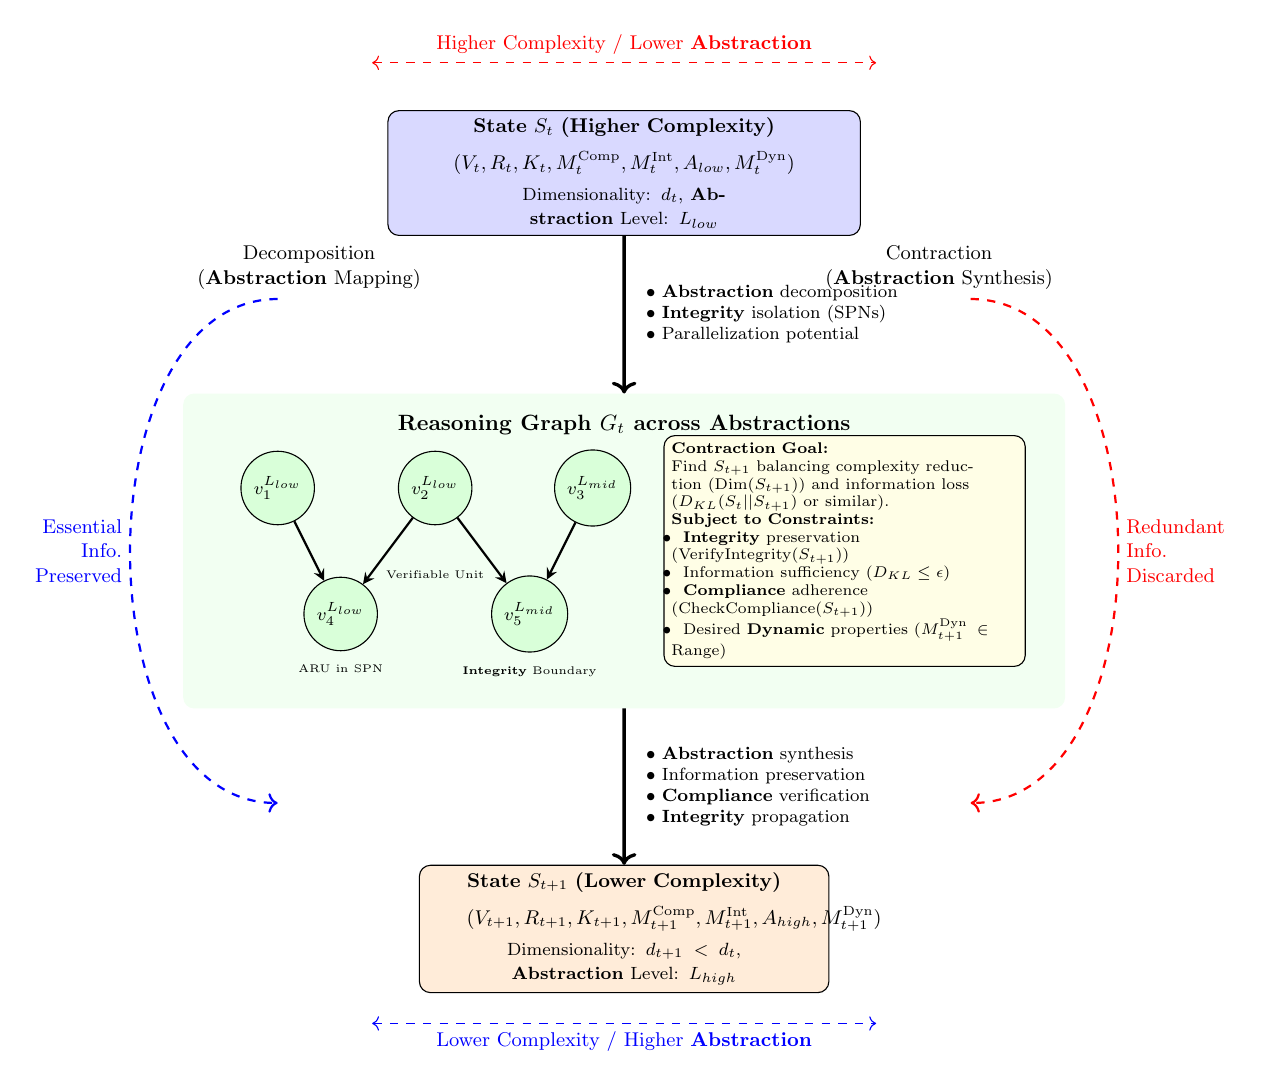
\begin{tikzpicture}[
			scale=0.8,
			transform shape,
			block/.style={rectangle, draw, rounded corners, minimum width=3.5cm, minimum height=1.8cm, text width=3.3cm, align=center, font=\small},
			state/.style={block, fill=blue!15},
			dag/.style={circle, draw, minimum size=0.8cm, font=\footnotesize},
			dep/.style={->, >=stealth, thick},
			phase/.style={draw=none, text=black, rounded corners, minimum width=2.5cm, minimum height=0.7cm, align=center, font=\small},
			highlight/.style={thick, dashed, rounded corners=5pt, draw=gray!60}
			]
			
			% Top state - high dimensional / low abstraction
			\node[state, minimum width=7.5cm, text width=5.5cm] (st) at (0,1) {\textbf{State $S_t$ (Higher Complexity)}\\[0.2cm] $(V_t, R_t, K_t, M_t^{\text{Comp}}, M_t^{\text{Int}}, A_{low}, M^{\text{Dyn}}_t)$\\[0.1cm] \footnotesize{Dimensionality: $d_t$, \Abstraction\ Level: $L_{low}$}};
			
			% Process phases
			\node[phase] at (-5,-.5) {Decomposition\\(\Abstraction\ Mapping)};
			\node[phase] at (5,-.5) {Contraction\\(\Abstraction\ Synthesis)};
			
			% Middle DAG
			\begin{scope}[shift={(-3,-5)}]
				% Background for DAG
				\fill[rounded corners, fill=green!5] (-4,-2.5) rectangle (10,2.5);
				\node[align=center] at (3,2) {\textbf{Reasoning Graph $G_t$ across Abstractions}};
				
				% DAG nodes (ARUs)
				\node[dag, fill=green!15] (v1) at (-2.5,1) {$v_1^{L_{low}}$};
				\node[dag, fill=green!15] (v2) at (0,1) {$v_2^{L_{low}}$};
				\node[dag, fill=green!15] (v3) at (2.5,1) {$v_3^{L_{mid}}$}; % Mid-level
				\node[dag, fill=green!15] (v4) at (-1.5,-1) {$v_4^{L_{low}}$};
				\node[dag, fill=green!15] (v5) at (1.5,-1) {$v_5^{L_{mid}}$};
				
				% DAG edges (representing dependencies / OAMI flow)
				\draw[dep] (v1) -- (v4);
				\draw[dep] (v2) -- (v4);
				\draw[dep] (v2) -- (v5); % Cross-level dependency implied
				\draw[dep] (v3) -- (v5);
				
				% Node labels
				\node[font=\tiny, align=center, below=0.1cm of v4] {ARU in SPN};
				\node[font=\tiny, align=center, below=0.6cm of v2] {Verifiable Unit};
				\node[font=\tiny, align=center, below=0.1cm of v5] {\Integrity\ Boundary};
			\end{scope}
			
			% Bottom state - reduced dimensionality / higher abstraction
			\node[state, fill=orange!15, minimum width=6.5cm, text width=5cm] (st1) at (0,-11) {\textbf{State $S_{t+1}$ (Lower Complexity)}\\[0.2cm] $(V_{t+1}, R_{t+1}, K_{t+1}, M_{t+1}^{\text{Comp}}, M_{t+1}^{\text{Int}}, A_{high}, M^{\text{Dyn}}_{t+1})$\\[0.1cm] \footnotesize{Dimensionality: $d_{t+1} < d_t$, \Abstraction\ Level: $L_{high}$}};
			
			% Main arrows
			\draw[->, very thick] (st) -- node[right, align=left, font=\footnotesize] {
				\begin{tabular}{l}
					$\bullet$ \Abstraction\ decomposition\\
					$\bullet$ \Integrity\ isolation (SPNs)\\
					$\bullet$ Parallelization potential
				\end{tabular}
			} (0,-2.5);
			
			\draw[->, very thick] (0,-7.5) -- node[right, align=left, font=\footnotesize] {
				\begin{tabular}{l}
					$\bullet$ \Abstraction\ synthesis\\
					$\bullet$ Information preservation\\
					$\bullet$ \textbf{Compliance} verification\\
					$\bullet$ \Integrity\ propagation
				\end{tabular}
			} (st1);
			
			% Dimensionality / Abstraction visualization
			\draw[<->, dashed, red] (-4,2.75) -- node[above, font=\small] {Higher Complexity / Lower \Abstraction} (4,2.75);
			\draw[<->, dashed, blue] (-4,-12.5) -- node[below, font=\small] {Lower Complexity / Higher \Abstraction} (4,-12.5);
			
			% Optimization problem - Simplified text (adapted from OLD Eq 2.21)
			\node[draw, fill=yellow!10, rounded corners, align=left, font=\scriptsize, text width=5.5cm] at (3.5,-5) {
				\textbf{Contraction Goal:}\\
				Find $S_{t+1}$ balancing complexity reduction ($\text{Dim}(S_{t+1})$) and information loss ($D_{KL}(S_t || S_{t+1})$ or similar).\\
				\textbf{Subject to Constraints:}\\
				~~\llap{$\bullet$~~}\Integrity\ preservation ($\text{VerifyIntegrity}(S_{t+1})$)\\
				~~\llap{$\bullet$~~}Information sufficiency ($D_{KL} \le \epsilon$)\\
				~~\llap{$\bullet$~~}\textbf{Compliance} adherence ($\text{CheckCompliance}(S_{t+1})$)\\
				~~\llap{$\bullet$~~}Desired \textbf{Dynamic} properties ($M^{\text{Dyn}}_{t+1} \in \text{Range}$)
			};
			
			% Information flow
			\draw[->, thick, blue, dashed] (-5.5,-1) to[out=180,in=180] node[left, align=right, font=\small] {Essential\\Info.\\Preserved} (-5.5,-9);
			\draw[->, thick, red, dashed] (5.5,-1) to[out=0,in=0] node[right, align=left, font=\small] {Redundant\\Info.\\Discarded} (5.5,-9);
			
		\end{tikzpicture}
		\caption[Decomposition-Contraction Cycle]{Decomposition-Contraction Cycle for Abstraction Management and Complexity Reduction. Transforms state $S_t$ into a DAG $G_t$ of ARUs (executed in SPNs, potentially spanning multiple \Abstraction\ levels), then contracts $G_t$ results into a less complex state $S_{t+1}$, preserving essential information while managing complexity. The process is subject to \Integrity, \textbf{Compliance}, and \textbf{Dynamic} constraints, guided by an optimization goal balancing complexity and information fidelity.}
		\label{fig:decomposition-contraction}
	\end{figure}
	
	\subsection{Information Preservation and Integrity Guarantees}
	\label{sec:2-4-5_and_6}
	
	The contraction process $C: G_t \rightarrow S_{t+1}$ must selectively embed information to preserve fidelity while reducing complexity. This involves optimizing the trade-off between state size and information loss (e.g., minimizing KL divergence or maximizing mutual information with future relevant variables), subject to hard constraints ensuring \Integrity, \textbf{Compliance}, valid \Abstraction\ mapping, and desirable system \Dynamics. This contrasts with reasoning chains that accumulate history, potentially leading to computational inefficiency \citep{Teng2025AtomOfThoughtsRef}. This optimization might be implemented within a coordinating Meta-Process.
	
	Theoretical guarantees underpin this process, adapted from information theory and security principles:
	
	\begin{theorem}[Sufficiency of Markovian State]
		\label{thm:sufficiency}
		Under specified assumptions about the reasoning process (ARUs) and the decomposition-contraction mechanism (optimizing information flow \citep{Tishby2000InformationBottleneck}), there exists a finite-dimensional Markovian state representation $S_t$ such that reasoning based on $S_t$ achieves expected utility within $\epsilon$ of reasoning with the complete history, while satisfying defined \Integrity\ and \textbf{Compliance} constraints enforced by the framework.
	\end{theorem}
	\begin{proof}
		(Sketch) Leverages concepts similar to the information bottleneck method, showing that a compressed state representation $S_{t+1}$ derived via contraction $C$ can preserve relevant information for future decisions up to a certain fidelity $\epsilon$, constrained by compliance and integrity requirements. Formal proof deferred to Appendix~\ref{app:proof_sufficiency_markovian}.
	\end{proof}
	
	\begin{theorem}[Integrity Preservation in Contraction]
		\label{thm:integrity_preservation}
		If the initial state $S_t$ has verified \Integrity\ (e.g., composed from verified CSTs), and all ARUs $A_v$ in the reasoning graph $G_t$ execute with verifiable \Integrity\ within SPNs (satisfying $\mathcal{I}_{A_v}^{\text{Int}}$), and the contraction function $C$ (e.g., implemented in a Meta-Process) itself preserves integrity (operates correctly on verified inputs), then the resulting state $S_{t+1} = C(G_t)$ maintains verifiable \Integrity\ (e.g., can be stored as a new CST).
	\end{theorem}
	\begin{proof}
		(Sketch) Proceeds by showing that each step (ARU execution in SPN, secure transmission of results via OAMI, result synthesis by $C$) maintains integrity properties, relying on the guarantees of the SDS execution environment. Formal proof deferred to Appendix~\ref{app:proof_integrity_preservation}.
	\end{proof}
	
	\subsection{Integrity Implications of Atomic Reasoning}
	\label{sec:2-4-8}
	
	The ARU-based approach, executed within the SDS, enhances overall system \Integrity\ through several mechanisms:
	\begin{itemize}
		\item \textbf{Reduced Attack Surface}: Smaller, well-defined units (ARUs within SPNs) are easier to secure and verify than monolithic components.
		\item \textbf{Enhanced Verifiability}: Independent verification of ARU specifications and runtime integrity checks within SPNs simplifies assurance, potentially using ZKML \citep{Peng2025ZKMLSurvey}.
		\item \textbf{Containment}: Isolation within SPNs helps contain breaches or failures.
		\item \textbf{Auditable Chains}: The reasoning graph $G_t$ provides an explicit, potentially verifiable trace of computation via OAMI logs and SPN execution records.
		\item \textbf{Secure Composition}: Formal rules ($\mathcal{CM}$) govern how ARUs are composed via OAMI, preserving integrity across interactions.
	\end{itemize}
	
	\begin{theorem}[Integrity Composition of ARUs]
		\label{thm:aru_integrity_composition}
		If individual ARUs $\{A_i\}$ executed within SPNs for a reasoning graph $G_t$ satisfy their respective \Integrity\ invariants $\mathcal{I}_i^{\text{Int}}$, and their composition via OAMI follows integrity-preserving rules $\mathcal{I}_{\text{comp}}^{\text{Int}}$ (enforced by the SDS/OAMI protocol checks), then the composed reasoning step $T: S_t \rightarrow S_{t+1}$ maintains computational \Integrity.
	\end{theorem}
	\begin{proof}
		(Sketch) Uses induction on the structure of $G_t$, showing that integrity is preserved at each composition step (ARU execution and OAMI transfer). Formal proof deferred to Appendix~\ref{app:proof_aru_integrity_composition}.
	\end{proof}
	
	\section{Learning within the Open AMI Framework}
	\label{sec:2-5-new}
	
	Learning is a fundamental process within Open AMI, enabling systems to adapt, improve, and acquire knowledge from data and experience. Unlike traditional ML pipelines where trustworthiness is often assessed post-hoc, Open AMI treats learning itself as a core process executed within SPNs, subject to the framework's four pillars (\Compliance, \Integrity, \Abstraction, \Dynamics) as detailed in Chapter~\ref{ch:machine_learning}. This section outlines the theoretical integration, drawing on research in trustworthy and adaptive learning.
	
	\subsection{Learning as a Compliant, Verifiable Process}
	\label{sec:2-5-1-new}
	
	Learning, whether supervised, unsupervised, or reinforcement-based, involves updating system state (e.g., model parameters within an SPN, knowledge structures managed via OAMI) based on data. In Open AMI, this update process itself must adhere to strict requirements enforced by the SDS and Governance layers:
	
	\begin{itemize}
		\item \textbf{Compliance:} The learning process (executed in an SPN) must respect all relevant constraints from the Compliance Manifest ($\mathcal{CM}$, Chapter~\ref{ch:compliance}). This includes:
		\begin{itemize}
			\item \textit{Data Compliance:} Using only data whose sourcing and handling satisfy $\mathcal{CM}$ rules (verified via provenance checks, Sec~\ref{sec:4-5}).
			\item \textit{Algorithmic Compliance:} Ensuring the learning algorithm itself (code running in SPN) does not introduce unfair biases or violate safety constraints (verified via static analysis or runtime checks against $\mathcal{CM}$, Sec~\ref{sec:4-4}). This may involve using constrained learning techniques \citep{Constraint_RL_Survey_2024} or Safe RLHF approaches \citep{Dai_Safe_RLHF_2023}.
			\item \textit{Outcome Compliance:} Monitoring and guiding the learning process (potentially via Meta-Process interactions) to favor models whose behavior, when deployed, is expected to be compliant.
		\end{itemize}
		\item \textbf{Integrity:} The learning process must be verifiable and robust against manipulation or errors. This includes:
		\begin{itemize}
			\item \textit{Data Integrity:} Ensuring the training data (accessed by the SPN) is accurate, complete, and hasn't been tampered with (verified via SDS mechanisms, Sec~\ref{sec:4-5-2}).
			\item \textit{Algorithmic Integrity:} Verifying the correct implementation and execution of the learning algorithm within the SPN (e.g., via code signing, runtime attestation, or verifiable computation proofs like PoL \citep{Jia2021ProofOfLearning} or ZKPs \citep{Peng2025ZKMLSurvey} managed by SDS). Reproducibility is a key goal.
			\item \textit{Model Integrity:} Ensuring the resulting model updates (e.g., parameters, checkpoints stored by the SPN) are protected using cryptographic hashes or signatures managed by the SDS.
		\end{itemize}
	\end{itemize}
	
	\begin{definition}[Compliant Learning Process with Integrity]
		\label{def:compliant_learning}
		A learning process $L: (S_t, D_t) \rightarrow S_{t+1}$ executed within an SPN updates the system state $S_t$ (including model parameters $\theta_t$) based on data $D_t$ to produce a new state $S_{t+1}$. This process is compliant and maintains integrity if:
		\begin{align}
			&\text{VerifyCompliance}(D_t, \mathcal{CM}) = \text{true} \label{eq:learn_data_comp} \\
			&\text{VerifyIntegrity}(D_t) = \text{true} \label{eq:learn_data_int} \\
			&\text{VerifyCompliance}(L, \mathcal{CM}) = \text{true} \quad (\text{e.g., checks on algorithm implementation within SPN}) \label{eq:learn_algo_comp} \\
			&\text{VerifyIntegrity}(L, S_t, D_t) = \text{true} \quad (\text{e.g., proof of correct SPN execution via SDS}) \label{eq:learn_algo_int} \\
			&(\text{IsCompliant}(S_t) \land \text{HasIntegrity}(S_t)) \implies (\text{IsCompliant}(S_{t+1}) \land \text{HasIntegrity}(S_{t+1})) \label{eq:learn_state_preservation}
		\end{align}
		The process operates across defined \Abstraction\ levels (e.g., learning features vs. learning high-level rules) and its \Dynamics\ (e.g., convergence rate, stability, generalization performance) are monitored by the Governance Layer via reports from the SPN/Meta-Process.
	\end{definition}
	
	\subsection{Learning, Abstraction, and Knowledge Representation}
	\label{sec:2-5-2-new}
	
	Learning interacts deeply with the framework's concepts of \Abstraction\ and knowledge representation (Sec~\ref{sec:2-3}):
	\begin{itemize}
		\item \textbf{Learning at Multiple Abstraction Levels:} Models within SPNs might learn representations at different levels of detail. Open AMI's \Abstraction\ tools (e.g., via Meta-Processes or dedicated analysis SPNs) aim to make these learned representations navigable and understandable, potentially identifying interpretable features using techniques like dictionary learning \citep{Anthropic_Decompose_2023}.
		\item \textbf{Data Abstraction:} Learning might occur on raw data or on abstracted summaries (e.g., embeddings generated by one SPN, used by another). The choice of \Abstraction\ level for training data impacts efficiency, robustness, and potential biases, governed by system configuration/\textbf{Compliance}.
		\item \textbf{Integrating Learned Knowledge:} Learned models or knowledge extracted from them (e.g., decision rules, embeddings, causal graphs) become objects within the Cognitive Map / Knowledge Structure $\mathcal{C}$ (Definition~\ref{def:knowledge_category}). Their integration via OAMI (\texttt{knowledge/update}) requires verification according to Definition~\ref{def:knowledge_integration}, ensuring the \Integrity\ of the knowledge base is maintained. This forms part of the agentic knowledge expansion process \citep{Buehler2025AgenticGraphRef}.
		\item \textbf{Learning from Verified Experience:} The concept of learning from past cases can be framed as a specific learning strategy implemented within an SPN. It relies on retrieving historical data (inputs $x$, outcomes $y$, context) whose \Integrity\ and \textbf{Compliance} status have been previously verified and logged by the SDS. The learning update is based only on these trustworthy records. This ensures learning from experience builds upon a foundation of verified information.
	\end{itemize}
	
	
	\subsection{Managing Learning Dynamics}
	\label{sec:2-5-3-new}
	
	Continuous or adaptive learning introduces complex system \Dynamics\ that must be actively managed by the Governance Layer (interacting with Meta-Processes and SPNs via OAMI) to ensure stability, robustness, and ongoing \textbf{Compliance}. This aligns with challenges identified in continual learning research, such as catastrophic forgetting and stability-plasticity trade-offs \citep{Wang2024ContinualLearningSurvey}.
	\begin{itemize}
		\item \textbf{Stability vs. Plasticity:} Balancing the ability to learn new information (plasticity) with the need to retain previous knowledge and maintain stable performance (stability). The Governance Layer monitors learning rates, performance metrics (reported by SPNs/Meta-Processes), and potential catastrophic forgetting, potentially adjusting learning parameters (e.g., regularization strengths) via OAMI control messages, using techniques like Elastic Weight Consolidation (EWC) \citep{Kirkpatrick2017OvercomingCF} managed within the learning SPN.
		\item \textbf{Convergence and Performance:} Monitoring learning progress (e.g., loss curves, validation metrics reported by the learning SPN) to ensure convergence towards desirable performance levels, while simultaneously ensuring that \textbf{Compliance} criteria (e.g., fairness metrics, safety bounds checked by the SPN or Meta-Process) are met. Learning may be paused or parameters adjusted if compliance boundaries are approached. The system must also manage robustness against distribution shifts, a significant challenge in adaptive systems \citep{DataDistributionShifts2022, AdditionalCitationRef53}.
		\item \textbf{Exploration vs. Exploitation (RL):} In reinforcement learning scenarios executed within SPNs interacting with OASIM or the real world (via OAMI), managing the trade-off between exploration and exploitation. Exploration strategies are constrained by safety rules defined in $\mathcal{CM}$ and enforced by the SPN or OASIM interface, potentially using safe RL techniques to manage exploration safely \citep{Constraint_RL_Survey_2024, Cao_PhyDRL_2024, AdditionalCitationRef16}. The Governance Layer may dynamically adjust exploration parameters (e.g., $\epsilon$) based on risk assessment and monitored system \Dynamics.
		\item \textbf{Feedback Loops:} Incorporating feedback (from human oversight via OAMI, environmental interaction, or internal monitoring) into the learning process in a controlled, compliant, and integrity-preserving manner. The \Integrity\ of the feedback source and mechanism (e.g., OAMI message integrity) is verified by the receiving SPN/Meta-Process. This could involve RLHF \citep{Dai_Safe_RLHF_2023} or Constitutional AI principles \citep{Bai2022ConstitutionalAI}.
	\end{itemize}
	The Governance Layer (Chapter~\ref{ch:compliance}) plays a key role in setting policies for and overseeing these learning \Dynamics, using the SDS infrastructure for monitoring and control.
	
	\subsection{Grounded Learning via Interaction and Simulation}
	\label{sec:2-5-4-new}
	
	Open AMI supports grounded learning, where models learn through interaction with environments (real or simulated via OASIM) rather than solely from static datasets. This is crucial for developing robust common sense and reliable interaction capabilities \citep{Physics-InspiredReasoning_Ref33}, enabled by the framework's architecture and aligning with research on digital twins and sim-to-real transfer \citep{Berg2025DigitalTwin, Li2025DigitalTwins, Josifovski_SCDA_2025}.
	\begin{itemize}
		\item \textbf{Embodied Learning:} Physical agents operating within the Open AMI framework (with logic in SPNs) can learn through interaction, leveraging standardized sensor/actuator protocols defined by OAMI (Appendix~\ref{app:protocol_spec}, potentially Sec B.7 extensions) and OASIM (Appendix~\ref{app:simulation_subsystem}) for the physical interface. All interactions are subject to runtime \textbf{Compliance} checks (e.g., safety limits enforced by the agent's SPN or the actuator interface).
		\item \textbf{Simulation-Based Learning (OASIM):} The OASIM subsystem provides a high-fidelity, verifiable (\Integrity) simulation environment accessible via OAMI. This allows for training models (e.g., RL agents within SPNs) through simulated experience, enabling safe exploration, hypothesis testing, and the generation of physically grounded training data whose parameters and \Integrity\ are known. The simulation itself operates under Open AMI principles. Techniques like domain randomization can be used within OASIM to improve sim-to-real transfer \citep{Tobin_Domain_Randomization_2017}.
	\end{itemize}
	
	\section{Prediction and Optimization within Constraints}
	\label{sec:2-6}
	
	Prediction and optimization are core AI capabilities, often relying on learned models executed within SPNs or implemented as ARUs. Within Open AMI, these operations are not performed in isolation but must strictly adhere to \textbf{Compliance} guarantees derived from $\mathcal{CM}$ and maintain computational \Integrity\ verified by the SDS.
	
	\subsection{Compliant Prediction Framework}
	\label{sec:2-6-1}
	
	Predictions generated by models must fall within acceptable boundaries defined by the system's compliance requirements, enforced at runtime.
	
	\begin{definition}[Compliance-Bounded Prediction]
		\label{def:compliant_prediction}
		A prediction $\hat{y}(t + \Delta t)$ generated by a model $M$ (executed in an SPN) based on input data $D_{\text{in}}$ (received via OAMI or local state) is compliance-bounded if:
		\begin{align}
			&\text{CheckCompliance}(\hat{y}(t + \Delta t), Y_{\text{compliant}}) = \text{true} \quad &&(\textbf{Compliance}: Output Constraints check by SPN) \label{eq:pred_output_comp}\\
			&\text{CheckCompliance}(\text{ModelUsageContext}(M, D_{\text{in}}), \mathcal{CM}) = \text{true} \quad &&(\textbf{Compliance}: Usage Context check by SPN/Meta-Process) \label{eq:pred_usage_comp}\\
			&\text{VerifyIntegrity}(\text{PredictionProcess}(M, D_{\text{in}})) = \text{true} \quad &&(\Integrity\ of SPN computation via SDS) \label{eq:pred_proc_int}
		\end{align}
		Here, $Y_{\text{compliant}}$ defines the set of permissible output values based on safety, ethical, or operational rules from $\mathcal{CM}$. Compliance also governs *how* and *in what context* the model is used (\ref{eq:pred_usage_comp}), checked against $\mathcal{CM}$. The process requires verified \Integrity\ of $M$ and $D_{\text{in}}$, and the prediction computation itself must be verifiable (\ref{eq:pred_proc_int}), potentially via ZKPs \citep{Peng2025ZKMLSurvey}. Predictions operate at specific \Abstraction\ levels, potentially specified in the request.
	\end{definition}
	
	\begin{theorem}[Compliance-Guaranteed Prediction]
		\label{thm:compliant_prediction_guarantee}
		If a model $M$ (with verified \Integrity) executes within an SPN that correctly enforces output constraints $Y_{\text{compliant}}$ and usage context rules from $\mathcal{CM}$ (Eq.~\ref{eq:pred_output_comp}, \ref{eq:pred_usage_comp}) on inputs $D_{\text{in}}$ (with verified \Integrity), and the prediction process maintains computational \Integrity\ (Eq.~\ref{eq:pred_proc_int}) via SDS mechanisms, then the resulting predictions $\hat{y}$ are compliance-bounded according to Definition~\ref{def:compliant_prediction}.
	\end{theorem}
	\begin{proof}
		(Sketch) Follows directly from the preconditions ensuring each component of Definition~\ref{def:compliant_prediction} is met through the enforcement mechanisms within the SPN and SDS. Formal proof deferred to Appendix~\ref{app:proof_compliant_prediction}.
	\end{proof}
	
	\subsection{Constrained Optimization}
	\label{sec:2-6-2}
	
	Optimization within Open AMI involves finding solutions (e.g., plans, parameters, actions) using algorithms (potentially implemented as ARUs within SPNs) that maximize some utility or minimize loss, while strictly satisfying all relevant \textbf{Compliance} constraints from $\mathcal{CM}$ and maintaining \Integrity. This relates to the field of constrained optimization and safe reinforcement learning \citep{Constraint_RL_Survey_2024}.
	
	\begin{definition}[Compliance-Constrained Optimization]
		\label{def:compliant_optimization}
		Find a solution $x^*$ within the feasible space $\mathcal{X}$ that optimizes an objective function $L(x)$, executed by an optimization process $O$ within the SDS:
		\begin{align}
			x^* = \arg\min_{x \in \mathcal{X}} L(x)
		\end{align}
		subject to the constraints that the solution $x^*$ and the context in which it is applied are compliant and maintain integrity, verified during or after the optimization process:
		\begin{align}
			&\text{CheckCompliance}(x^*, \text{Context}, \mathcal{CM}) = \text{true} \label{eq:opt_comp} \\
			&\text{VerifyIntegrity}(x^*, \text{Context}) = \text{true} \label{eq:opt_int}
		\end{align}
		Furthermore, the optimization algorithm $O$ itself must operate with computational \Integrity\ within its SPN, potentially adapt its strategy based on system \Dynamics\ (e.g., resource limits, time constraints), and respect relevant \Abstraction\ levels. Constraints might be handled using techniques like penalty methods, barrier functions, or projection operators implemented within the optimization ARU/SPN.
	\end{definition}
	
	\begin{theorem}[Optimization Compliance Guarantee]
		\label{thm:optimization_guarantee}
		If an optimization process $O$ running within the SDS starts in a state satisfying \textbf{Compliance} and \Integrity\ constraints, and each step of the optimization algorithm is guaranteed by its implementation and SDS enforcement to preserve these constraints (or project solutions back into the compliant/integral set), then the final solution $x^*$ found by the algorithm is guaranteed to be compliant and maintain integrity according to Definition~\ref{def:compliant_optimization}.
	\end{theorem}
	\begin{proof}
		(Sketch) Typically proven by induction on the steps of the optimization algorithm, assuming the preservation property holds for each step due to algorithmic design and runtime checks within the SPN. Formal proof deferred to Appendix~\ref{app:proof_optimization_guarantee}.
	\end{proof}
	
	\section{Guidance Functions: Steering Compliant Behavior}
	\label{sec:2-7}
	
	Guidance Functions are mechanisms within Open AMI, typically implemented by Meta-Processes or specialized SPNs, designed to steer system processes (including reasoning, learning, and action in other SPNs) towards desired goals while actively maintaining adherence to \textbf{Compliance} requirements from $\mathcal{CM}$ and preserving system \Integrity. They may adapt their operation based on the current system \Dynamics\ (monitored globally) and operate at specific \Abstraction\ levels, issuing commands via secure OAMI messages. These functions implement principles similar to ethical guardrails \citep{Sekrst2024Guardrails}.
	
	\subsection{Formal Definition}
	\label{sec:2-7-1}
	
	\begin{definition}[Compliant Guidance Function with Integrity]
		\label{def:guidance_function}
		A guidance function $G(t): S(t) \rightarrow \text{Command}$ maps the current system state $S(t)$ (aggregated from SPN reports and monitoring data) to a specific command (e.g., OAMI message to an SPN: adjust parameter $\Delta S$, execute action $a$) such that the resulting state $S'(t)$ or action sequence is guaranteed to be compliant and preserves integrity:
		\begin{align}
			(\text{IsCompliant}(S(t)) \land \text{HasIntegrity}(S(t))) \implies (\text{CheckCompliance}(\text{ResultOf}(Command)) \land \text{VerifyIntegrity}(Command))
		\end{align}
		The guidance command generated may depend on the dynamic state $M^{\text{Dyn}}_t$ (e.g., adapting control gain based on stability reported by SPNs) and operate at a specific \Abstraction\ level $A_t$. The function $G$ itself runs with computational \Integrity\ within its host (Meta-Process/SPN).
	\end{definition}
	
	\subsection{Types of Compliant Guidance Implementations}
	\label{sec:2-7-2}
	
	Open AMI can implement guidance using various techniques within SPNs or Meta-Processes, ensuring they operate within the framework's constraints:
	\begin{enumerate}
		\item \textbf{Rule-Based Guidance}: Applies actions (sent via OAMI) based on predefined rules derived from $\mathcal{CM}$, similar to the principles in Constitutional AI \citep{Bai2022ConstitutionalAI}. The Meta-Process/SPN executing the guidance function checks conditions based on received state information (verifying its \Integrity) and selects a compliant action.
		\begin{align}
			G_{\text{rule}}(s) = \begin{cases}
				\text{OAMI\_Cmd}(a_1(s)) & \text{if } c_1(s) \land \text{VerifyCompliant}(a_1(s), s, \mathcal{CM}) \land \text{VerifyIntegrity}(a_1(s)) \\
				\vdots \\
				\text{OAMI\_Cmd}(a_{\text{default}}(s)) & \text{otherwise (a safe default action command)}
			\end{cases} \label{eq:guidance_rule}
		\end{align}
		\item \textbf{Optimization-Based Guidance}: Computes actions by optimizing an objective function subject to compliance constraints (Def~\ref{def:compliant_optimization}), often projecting proposed actions onto the compliant state/action space before issuing commands via OAMI.
		\begin{align}
			G_{\text{opt}}(s) = \text{OAMI\_Cmd}(\text{Proj}_{\text{compliant}}\left( \arg\min_{a} L(s, a) \right)) \label{eq:guidance_opt}
		\end{align}
		where $\text{Proj}_{\text{compliant}}$ ensures the chosen action leads to a compliant state and maintains integrity.
		\item \textbf{Model Predictive Control (MPC) Guidance}: A Meta-Process plans a sequence of future actions by optimizing a predictive model (potentially involving OASIM calls via OAMI) over a finite horizon, subject to \textbf{Compliance} and \Integrity\ constraints at each predicted step, then issues the first action(s) via OAMI. This approach is used in safe control systems \citep{Berg2025DigitalTwin}.
		\begin{align}
			G_{\text{MPC}}(s_t) = \text{OAMI\_Cmd}(a_0^*) \quad \text{where } \{a_k^*\}_{k=0}^{N-1} = &\arg\min_{\{a_k\}} \sum_{k=0}^{N-1} \text{Cost}(\hat{s}_{t+k|t}, a_k) + \text{TerminalCost}(\hat{s}_{t+N|t}) \nonumber \\
			\text{s.t. } &\hat{s}_{t+k+1|t} = \text{PredictiveModel}(\hat{s}_{t+k|t}, a_k) \nonumber \\
			&\forall k, \text{CheckCompliance}(\hat{s}_{t+k|t}, a_k, \mathcal{CM}) = \text{true} \nonumber \\
			&\forall k, \text{VerifyIntegrity}(\hat{s}_{t+k|t}, a_k) = \text{true} \label{eq:guidance_mpc}
		\end{align}
	\end{enumerate}
	These methods ensure that system behavior is actively steered towards goals while remaining within trustworthy boundaries defined by $\mathcal{CM}$, orchestrated via OAMI commands within the secure SDS environment.
	
	\section{Emotional and Contextual Metadata Integration}
	\label{sec:2-8}
	
	To enable more nuanced and effective human-AI interaction, Open AMI incorporates mechanisms for representing, processing, and utilizing emotional and contextual metadata, where appropriate and explicitly permitted by \textbf{Compliance} policies. This integration must occur across relevant \Abstraction\ levels while strictly maintaining \textbf{Compliance} (e.g., respecting privacy, ensuring ethical use of sensitive information per $\mathcal{CM}$) and \Integrity\ (e.g., verifying the source and accuracy of metadata, ensuring integrity of inference models). The ethical implications of inferring and using emotional data are significant and must be carefully governed \citep{Sekrst2024Guardrails}.
	
	\subsection{Representation and Formal Model of Emotional Metadata}
	\label{sec:2-8-1}
	
	Open AMI adopts standard dimensional models for representing emotional states, such as Russell's Circumplex \citep{Russell1980Circumplex} or the Valence-Arousal (VA) / Valence-Arousal-Dominance (VAD) models (Zhang2024EmoSensing).
	
	\begin{definition}[Quantified Emotional State Vector]
		\label{def:emo_vector}
		An emotional state $\mathbf{E}$ inferred or provided at time $t$ is represented as a vector in a defined dimensional space, e.g., $\mathbf{E}(t) = [v, a]^T$ for Valence-Arousal, where $v, a \in [-1, 1]$. This vector is associated with metadata regarding its source, timestamp, inference confidence, and \Integrity\ proof.
	\end{definition}
	
	Integrating this emotional state into the system's reasoning or interaction logic (e.g., within an SPN responsible for Human-Machine Interface) requires rigorous verification:
	
	\begin{definition}[Compliant Emotional State Integration with Integrity]
		\label{def:emo_integration}
		Integrating an emotional state vector $\mathbf{E}$ (Def~\ref{def:emo_vector}) requires verification steps, typically performed by the receiving SPN:
		\begin{align}
			&\text{VerifyAuthenticity}(\text{Source}(\mathbf{E})) = \text{true} && \text{(\Integrity: Source verification, e.g., signed sensor data, authenticated user input via OAMI)} \\
			&\text{VerifyIntegrity}(\mathbf{E}) = \text{true} && \text{(\Integrity: Data not corrupted, inference model integrity verified if applicable)} \\
			&\text{CheckCompliance}(\text{Infer/Use}(\mathbf{E}), \text{UsageContext}, \mathcal{CM}_{\text{privacy}}, \mathcal{CM}_{\text{ethics}}) = \text{true} && \text{(\textbf{Compliance}: Checks against } \mathcal{CM} \text{ rules regarding inferring or using emotional data)}
		\end{align}
		The representation and processing of $\mathbf{E}$ may vary depending on the operational \Abstraction\ level. For instance, raw physiological sensor data (e.g., heart rate, EDA) might be processed by a dedicated SPN using a verified ML model (\Integrity, \textbf{Compliance}) to infer the VA vector (\Abstraction), which is then used by another SPN to modulate interaction style.
	\end{definition}
	
	
	\subsection{Contextual Awareness with Compliance Boundaries}
	\label{sec:2-8-2}
	
	Contextual information (e.g., location, time, social setting, task goal) is crucial for appropriate AI behavior. Integrating this context $\mathcal{C}(t)$ into the system state (e.g., within SPNs or Meta-Processes) requires strict adherence to \textbf{Compliance} and \Integrity.
	
	\begin{definition}[Compliant Contextual Integration with Integrity]
		\label{def:context_integration}
		Integrating contextual information $\mathcal{C}(t)$ (represented as structured data, potentially from sensors or databases accessed via OAMI) into the system state requires verification by the integrating component:
		\begin{align}
			&\forall c_i \in \mathcal{C}(t), \text{CheckCompliance}(\text{Access}(c_i), \text{SystemComponent}, \mathcal{CM}_{\text{access}}, \mathcal{CM}_{\text{privacy}}) = \text{true} && \text{(\textbf{Compliance}: Authorization \& Privacy check against } \mathcal{CM} \text{)} \\
			&\forall c_i \in \mathcal{C}(t), \text{VerifyProvenance}(c_i \text{ via metadata}) = \text{true} && \text{(\Integrity: Source tracking)} \\
			&\forall c_i \in \mathcal{C}(t), \text{VerifyIntegrity}(c_i \text{ via hash/signature}) = \text{true} && \text{(\Integrity: Data validity)}
		\end{align}
		Contextual information is managed across relevant \Abstraction\ levels (e.g., raw GPS coordinates vs. symbolic location label ``Office''). The choice of level impacts reasoning and potential \textbf{Compliance} implications (e.g., privacy sensitivity).
	\end{definition}
	
	\subsection{Usage within Open AMI}
	Emotional and contextual metadata, once integrated in a compliant and integrity-preserving manner, can inform various system functions:
	\begin{itemize}
		\item \textbf{Adaptive Interaction:} Adjusting communication style, response timing, or information presentation in human-AI interfaces based on inferred user emotional state or context (subject to strict \textbf{Compliance} rules in $\mathcal{CM}$).
		\item \textbf{Risk Assessment:} Using context (e.g., safety-critical environment) or emotional state (e.g., user distress) as input to dynamic risk assessment performed by the Governance Layer.
		\item \textbf{Personalization:} Tailoring system behavior or recommendations based on context (e.g., location, time of day), again strictly governed by \textbf{Compliance} policies regarding personalization and data usage.
		\item \textbf{Grounded Reasoning:} Providing situational awareness that grounds abstract reasoning processes in the current context.
	\end{itemize}
	The integration and use of such sensitive data must be explicitly defined and justified within the system's \Compliance\ Manifest ($\mathcal{CM}$) and implemented using the verifiable mechanisms of the SDS and OAMI.
	
	\section{Compliance Foundations and Formal Verification}
	\label{sec:2-9}
	
	The ethical and operational guidelines underpinning \textbf{Compliance} in Open AMI are formalized in the Compliance Manifest ($\mathcal{CM}$) to allow rigorous verification by mechanisms within the SDS and Governance Layer. This ensures system behavior aligns with specified requirements and relies on the \Integrity\ of the system state and verification processes. This addresses the AI specification challenge \citep{Kovac2025SpecGaming} by aiming for precise, machine-readable rules.
	
	\subsection{Formal Compliance Constraints}
	\label{sec:2-9-1}
	
	\begin{definition}[Compliance Constraint Satisfaction]
		\label{def:compliance_satisfaction}
		A system state $s$ (or action $a$) satisfies the set of compliance constraints $\mathcal{C}_{\text{Comp}}$ defined in the Compliance Manifest ($\mathcal{CM}$) if, for every applicable constraint $c \in \mathcal{C}_{\text{Comp}}$, the verification holds:
		\begin{align}
			\forall c \in \mathcal{C}_{\text{Comp}} \text{ applicable to } s, \text{VerifyConstraint}(s, c) = \text{true}
		\end{align}
		Constraints $c$ are formally specified (Def~\ref{def:compliance_constraint}), potentially using formal logic (e.g., temporal logic, predicate logic) or computational checks, defined at specific \Abstraction\ levels. Verification is performed by designated components (SPN checkers $A_n$, Meta-Processes) and relies on the verified \Integrity\ of the state $s$ (e.g., from CSTs) and the integrity of the verification function itself. The structure mirrors rule-based systems like Constitutional AI \citep{Bai2022ConstitutionalAI}.
	\end{definition}
	
	\begin{theorem}[Compliance Invariance]
		\label{thm:compliance_invariance}
		If an initial system state $s_0$ is compliant (satisfies Definition~\ref{def:compliance_satisfaction}), and all state transition functions $T$ applied by the system are compliance-preserving (i.e., runtime enforcement ensures $\text{IsCompliant}(s) \implies \text{IsCompliant}(T(s))$), then all reachable states of the system will remain compliant, assuming the operational \Integrity\ of the state representation and the transition enforcement mechanisms (SDS) is maintained.
	\end{theorem}
	\begin{proof}
		(Sketch) Standard proof by induction on the number of state transitions. Relies critically on the verification of transitions by SDS/Governance mechanisms referencing $\mathcal{CM}$ and the integrity of the state. Formal proof deferred to Appendix~\ref{app:proof_compliance_invariance}.
	\end{proof}
	
	\subsection{Bias Detection and Mitigation as Compliance}
	\label{sec:2-9-2}
	
	Ensuring fairness and preventing harmful bias is treated as a core \textbf{Compliance} requirement within Open AMI, formalized in $\mathcal{CM}$ and implemented via mechanisms detailed in Sec~\ref{sec:4-4}. Formal definitions are used to quantify fairness, aligning with standards demanding non-discrimination \citep{Navigating_AI_Conformity_2025}.
	
	\begin{definition}[Fairness Compliance (Example: Statistical Parity)]
		\label{def:fairness_compliance}
		A decision function $d$ (e.g., implemented by a model $M$ in an SPN) is $\epsilon$-fairness-compliant with respect to a protected attribute $a$ (e.g., race, gender) under the statistical parity criterion if the probability of a positive outcome is approximately equal across groups defined by $a$, as verified by a monitoring component using data with verified \Integrity:
		\begin{align}
			\max_{v_1, v_2 \in \text{Values}(a)} \left| P(d(x) = 1 | a(x) = v_1) - P(d(x) = 1 | a(x) = v_2) \right| \leq \epsilon
		\end{align}
		where $\epsilon$ is a predefined tolerance threshold from $\mathcal{CM}$. Verification requires data \Integrity\ (accurate labels for $a$ and outcomes) and operates within the \Abstraction\ framework (e.g., fairness measured at the level of individual decisions or aggregate statistics). Other fairness metrics (e.g., equal opportunity, equalized odds) can be similarly formalized in $\mathcal{CM}$. Bias mitigation procedures (detailed in Sec~\ref{sec:4-4}) are themselves treated as compliant processes requiring \Integrity.
	\end{definition}
	
	\section{Holistic Multi-Component Collaboration}
	\label{sec:2-10}
	
	Open AMI is designed to support collaboration among multiple components (SPNs, Meta-Processes, potentially external systems via gateways), ensuring that interactions via the OAMI protocol are \textbf{Compliant} with policies in $\mathcal{CM}$ and maintain end-to-end \Integrity. Collaboration might involve coordinating actions based on collective system \Dynamics\ across shared \Abstraction\ models, including scenarios like federated or collaborative learning managed by Meta-Processes, or agentic graph expansion where components recursively build shared knowledge structures \citep{Buehler2025AgenticGraphRef}. This requires robust communication and coordination protocols, as highlighted in multi-agent system research \citep{AdditionalCitationRef55, Meta_CICERO_2022}.
	
	\subsection{Compliant Multi-Component Interaction Model}
	\label{sec:2-10-1}
	
	\begin{definition}[Compliant Component Communication with Integrity]
		\label{def:multi_comp_comm}
		Communication $\text{Msg}_{i,j}$ between components $C_i$ (in SPN $i$) and $C_j$ (in SPN $j$) via the OAMI protocol (Appendix~\ref{app:protocol_spec}) over SDS secure channels must satisfy:
		\begin{align}
			&\text{VerifyAuthenticity}(C_i, C_j \text{ via mTLS/tokens}) = \text{true} && (\Integrity: Authentication) \\
			&\text{VerifyIntegrity}(\text{Msg}_{i,j} \text{ via TLS MACs / msg signatures}) = \text{true} && (\Integrity: Message content unchanged) \\
			&\text{CheckCompliance}(\text{Msg}_{i,j}, \text{Policy}_{\text{comm}} \text{ from } \mathcal{CM}, \text{Context}) = \text{true} && (\textbf{Compliance}: Adheres to comms policy, checked by receiver/Meta-Process)
		\end{align}
		Shared understanding and effective collaboration often rely on components operating with or mapping between common \Abstraction\ levels (e.g., using shared ontologies defined in a KG accessible via OAMI).
	\end{definition}
	
	\subsection{Conflict Resolution with Provable Compliance Properties}
	\label{sec:2-10-2}
	
	When multiple components (SPNs) have conflicting goals or propose conflicting actions (detected by a coordinating Meta-Process), formal conflict resolution mechanisms, specified in $\mathcal{P}_{\text{conflict}} \subseteq \mathcal{CM}$, are needed. These mechanisms must ensure outcomes satisfy overarching \textbf{Compliance} requirements and that the resolution process itself (executed by the Meta-Process) maintains \Integrity. Handling such conflicts is a recognized challenge in ethical AI design \citep{Sekrst2024Guardrails}.
	
	\begin{definition}[Compliant Conflict Resolution]
		\label{def:compliant_conflict_resolution}
		A conflict resolution process $R$, executed by a Meta-Process, takes conflicting goals/actions $G_i, G_j$ and produces a resolution $Res(G_i, G_j)$ such that:
		\begin{align}
			&\text{CheckCompliance}(Res(G_i, G_j), \mathcal{P}_{\text{conflict}}) = \text{true} \label{eq:conflict-comp} \\
			&\text{VerifyIntegrity}(R) = \text{true} \label{eq:conflict-int}
		\end{align}
		where $\mathcal{P}_{\text{conflict}} \subseteq \mathcal{CM}$ defines priority rules (Def~\ref{def:priority_relation}). Resolution aims to satisfy highest priority constraints, possibly using techniques like lexicographic ordering. The process $R$ runs with computational \Integrity, and its outcome/rationale is logged securely by SDS.
	\end{definition}
	
	\section{Operational Self-Awareness and Monitoring}
	\label{sec:2-11}
	
	Open AMI systems are designed to maintain awareness of their own operational state, facilitated by the SDS monitoring architecture (Sec~\ref{sec:3-5-1}) reporting to the Governance Layer. This includes monitoring their \textbf{Compliance} posture, \Integrity\ status (of data, components, processes), current usage of \Abstraction\ levels, and key system \Dynamics\ indicators (like stability, performance, learning progress).
	
	\subsection{Formal Monitoring Model}
	\label{sec:2-11-1}
	
	\begin{definition}[System State Assessment]
		\label{def:state_assessment}
		An assessment function $\Sigma$, typically executed within the Governance Layer (or supporting Meta-Processes), evaluates the current aggregated system state $s$ (based on \Integrity-verified reports from SPNs/Meta-Processes) against relevant policies $\mathcal{P}$ (including subsets of $\mathcal{CM}$ and operational policies):
		\begin{align}
			\Sigma(s, \mathcal{P}) = \langle \text{Status}_{\text{Comp}}, \text{Status}_{\text{Int}}, \text{Status}_{\text{Abs}}, \text{Status}_{\text{Dyn}} \rangle
		\end{align}
		where each status component indicates the current state relative to desired operational ranges or compliance rules. For example:
		\begin{align}
			\text{Status}_{\text{Comp}} \in \{\text{Compliant}, \text{Warning}(W), \text{Violation}(V)\}
		\end{align}
		The assessment relies on monitoring data whose own \Integrity\ must be ensured by the SDS. It aggregates information potentially across multiple \Abstraction\ levels and tracks relevant \Dynamics.
	\end{definition}
	
	\subsection{Real-Time Response}
	\label{sec:2-11-2}
	
	Based on the state assessment $\Sigma(s)$, response mechanisms within the Governance Layer can be triggered, issuing commands via OAMI to relevant Meta-Processes or SPNs.
	
	\begin{definition}[Compliance/Dynamics Action Function]
		\label{def:response_action}
		An action function $\Lambda$, executed by the Governance Layer or designated Meta-Processes, maps the assessed system state $\Sigma(s)$ to a set of response actions $\mathcal{A}$ (typically OAMI commands):
		\begin{align}
			\Lambda: \Sigma(s) \rightarrow \mathcal{A}
		\end{align}
		Actions $\mathcal{A}$ are selected based on detected violations (e.g., $V$ in $\text{Status}_{\text{Comp}}$), integrity failures ($\text{Status}_{\text{Int}}$), deviations from desired dynamics ($\text{Status}_{\text{Dyn}}$), or inappropriate abstraction usage ($\text{Status}_{\text{Abs}}$). Examples include: adjusting learning rates in an SPN, triggering safety stops via OAMI command, isolating a compromised SPN, switching system operation to a different abstraction level, alerting human operators. All response actions must themselves be compliant and preserve system \Integrity\ (verified before issuing).
	\end{definition}
	
	\section{Comparative Analysis and Theoretical Limitations}
	\label{sec:2-12}
	
	This section evaluates Open AMI's theoretical foundations in comparison to alternatives and acknowledges inherent limitations.
	
	\subsection{Comparative Theoretical Analysis}
	\label{sec:2-12-1}
	
	Table~\ref{tab:theoretical-strengths-revised} summarizes the theoretical strengths and limitations of Open AMI, reflecting its focus on integrating trustworthiness pillars throughout the AI/ML lifecycle. The framework's strength lies in this integration, aiming to provide verifiable trustworthiness by design.
	
	\begin{table}[ht]
		\centering
		\caption[Theoretical Strengths and Limitations of Open AMI]{Theoretical Strengths and Limitations of Open AMI}
		\label{tab:theoretical-strengths-revised}
		\begin{tabular}{@{}lll@{}}
			\toprule
			\textbf{Pillar/Aspect} & \textbf{Open AMI Strengths} & \textbf{Limitations \& Research Challenges} \\
			\midrule
			\textbf{Compliance} & Integrated by design ($\mathcal{CM}$, SDS enforcement) & Specification completeness \citep{Kovac2025SpecGaming}; Verifying emergence \\
			\Integrity\ & Verifiable computation/data (SDS, crypto, SPNs) & Overhead; Scalability of verification (esp. ZKP/MPC \citep{Peng2025ZKMLSurvey}) \\
			\Abstraction\ & Explicit management (Cognitive maps, Decomp/Contract) & Defining meaningful abstractions; Interpretability \citep{Anthropic_Decompose_2023} vs. fidelity trade-off \\
			\Dynamics & Framework for managing adaptation/stability (Gov. Layer) & Characterizing/controlling complex non-linear dynamics \citep{Wang2024ContinualLearningSurvey} \\
			Learning & Compliant, Verifiable (SDS), Grounded (OASIM) & Balancing safety/exploration \citep{Constraint_RL_Survey_2024}; Verifying continuously learned behavior \\
			Reasoning & Verifiable units (ARUs); Markovian states (\citep{Teng2025AtomOfThoughtsRef}); Physics-inspired potential (OASIM \citep{Cao_PhyDRL_2024}) & Scalability; Rigor/utility of physics mapping; Composition guarantees (\citep{Buehler2025AgenticGraphRef}) \\
			Overall & Unified trustworthy AI/ML framework & Interactions between pillars; Practical implementation complexity; Tooling maturity \\
			\bottomrule
		\end{tabular}
	\end{table}
	
	\subsection{Known Theoretical Limitations}
	\label{sec:2-12-2}
	
	Despite its comprehensive design, Open AMI faces theoretical limitations that represent active research areas:
	
	\begin{enumerate}
		\item \textbf{Verification Scalability:} Formally verifying large ML models or complex, adaptive processes for full \textbf{Compliance} and \Integrity\ remains computationally expensive \citep{Peng2025ZKMLSurvey}. Approximate or statistical verification methods, managed within the framework, may be necessary in practice.
		\item \textbf{Specification Completeness:} Fully specifying all relevant \textbf{Compliance} rules in $\mathcal{CM}$ (especially nuanced ethical considerations \citep{Sekrst2024Guardrails}), desired learning \Dynamics, and ideal \Abstraction\ mappings for complex, open-ended systems is inherently difficult, representing the core "AI specification problem" \citep{Kovac2025SpecGaming}.
		\item \textbf{Physics-Reasoning Mapping Rigor:} While architecturally supported via OASIM, establishing useful, non-superficial, and computationally efficient mappings between reasoning tasks and physical dynamics requires significant theoretical and empirical work \citep{Physics-InspiredReasoning_Ref11}.
		\item \textbf{Control of Complex Dynamics:} Robustly controlling adaptation, stability, and exploration in high-dimensional, non-stationary learning systems, even with the framework's monitoring and control loops, is an ongoing research challenge in control theory and ML \citep{Wang2024ContinualLearningSurvey}.
		\item \textbf{Abstraction Fidelity vs. Interpretability:} Creating abstractions (e.g., via Decomposition-Contraction or KG structuring) that significantly reduce complexity while retaining sufficient fidelity for downstream tasks and providing genuine human interpretability is hard, although techniques like feature decomposition show promise \citep{Anthropic_Decompose_2023}.
		\item \textbf{Emergent Behaviors:} Interactions between multiple components via OAMI can lead to unexpected emergent behaviors (as seen in self-organizing KGs \citep{Buehler2025AgenticGraphRef}) that may impact \textbf{Compliance} or stability in ways not easily predicted from individual component analysis. Requires robust system-level monitoring and potentially multi-agent safety protocols \citep{DoriHacohen2025Misalignment}.
		\item \textbf{Pillar Trade-offs:} There are inherent trade-offs between the pillars (e.g., \textbf{Compliance} vs. performance, \Integrity\ overhead vs. speed, \Abstraction\ level vs. fidelity). Formalizing and managing these trade-offs optimally within the Governance Layer requires further research \citep{Sekrst2024Guardrails}.
		\item \textbf{Human Alignment Fidelity:} Formalizing human values and preferences into $\mathcal{CM}$ (\textbf{Compliance}) remains an incomplete process, requiring ongoing interaction, feedback mechanisms (Sec~\ref{sec:4-7}), and potentially value learning techniques \citep{Kovac2025SpecGaming}.
		\item \textbf{Markovian Assumption Limits:} While aiming for Markovian state transitions can improve efficiency \citep{Teng2025AtomOfThoughtsRef}, strict adherence may not always be possible or optimal, potentially discarding useful historical context. Balancing state atomicity with necessary history is a challenge.
	\end{enumerate}
	
	\section{Summary and Integration with Architectural Framework}
	\label{sec:2-13}
	
	This chapter presented the theoretical foundations of Open AMI, establishing a formal basis for building trustworthy AI/ML systems. By integrating Process Theory, Cognitive Mapping analogues inspired by self-organizing knowledge networks \citep{Buehler2025AgenticGraphRef}, structured Atomic Reasoning Units (ARUs), Markovian state transition concepts \citep{Teng2025AtomOfThoughtsRef}, and principles for compliant learning within the four pillars of \textbf{Compliance}, \Integrity, \Abstraction, and system \Dynamics, Open AMI provides rigorous underpinnings for developing advanced AI that learns, reasons, and acts reliably and responsibly.
	
	These theoretical components directly inform the Open AMI architecture described in subsequent chapters:
	\begin{itemize}
		\item \textbf{Process Theory} provides the formal models for system activities, including learning. These processes are instantiated and managed by Secure Process Nodes (SPNs) and Meta-Processes within the Secure Distributed System (SDS, Chapter~\ref{ch:secure_distributed_system}), ensuring \textbf{Compliance} and \Integrity.
		\item \textbf{Cognitive Mapping} informs the design of knowledge representation and integration mechanisms within the Intelligence Layer (potentially using KGs managed by SPNs), supporting reasoning and learning across different \Abstraction\ levels via OAMI interactions, potentially enabling emergent knowledge structures \citep{Buehler2025AgenticGraphRef}.
		\item \textbf{Atomic Reasoning} (ARUs) defines the verifiable computational units executed within SPNs in the Operational Layer (SDS), ensuring computational \Integrity\ and potentially leveraging \textbf{physics-inspired dynamics} via OASIM (Appendix~\ref{app:simulation_subsystem}). The Decomposition-Contraction cycle provides a mechanism for managing complexity and \Abstraction\ coordinated by Meta-Processes, aiming for efficient state transitions \citep{Teng2025AtomOfThoughtsRef}.
		\item The \textbf{Foundations for Compliant Learning} (Sec~\ref{sec:2-5-new}) guide the design, implementation, and management of ML processes within the Intelligence Layer (detailed in Chapter~\ref{ch:machine_learning}), ensuring they operate under the framework's \textbf{Compliance}, \Integrity, and \Dynamics\ constraints enforced by the SDS and Governance layers.
		\item \textbf{Guidance Functions} (Sec~\ref{sec:2-7}) enable the Governance and Intelligence Layers (specifically Meta-Processes/SPNs) to steer system behavior, including learning processes, while maintaining \textbf{Compliance}, using OAMI for control.
		\item \textbf{Operational Self-Awareness} principles (Sec~\ref{sec:2-11}) inform the monitoring functions within the Governance Layer, tracking \textbf{Compliance} status, \Integrity, \Abstraction\ usage, and system \Dynamics\ based on data aggregated from the SDS.
	\end{itemize}
	
	This framework aims to move beyond the limitations of current AI development practices by embedding trustworthiness principles directly into the theoretical and architectural fabric of AI/ML systems, paving the way for more capable, reliable, and aligned artificial intelligence.
	
		\chapter{Machine Learning Paradigms in Open AMI} % Corrected Chapter Title
	\label{ch:machine_learning}
	
	\section{Introduction: Trustworthy Machine Learning Lifecycle} % Corrected Section Title and Numbering
	\label{sec:3-1} % Adjusted label to match new sectioning scheme
	
	Machine Learning (ML) is a core component of modern AI, enabling systems to learn from data and improve performance over time. The Open AMI framework is designed not merely to *use* pre-trained ML models, but to provide a comprehensive, trustworthy environment for the entire ML lifecycle. This encompasses data acquisition and preparation, model training and validation, deployment, monitoring, and continuous adaptation or retraining, all executed within the secure and verifiable context provided by the Open AMI architecture, particularly the Secure Distributed System (SDS) and governed by the Compliance Manifest ($\mathcal{CM}$). This lifecycle approach aligns with emerging standards requiring AI conformity assessments \citep{Navigating_AI_Conformity_2025} and responsible AI governance processes \citep{Responsible_AI_Governance_Review_2024}.
	
	This chapter details how various ML paradigms—including supervised, unsupervised, reinforcement, continuous, and federated learning—are conceptualized, implemented, managed, and verified within the Open AMI framework. The emphasis is on how Open AMI's four pillars (\Compliance, \Integrity, \Abstraction, \Dynamics) are applied throughout the ML lifecycle, leveraging specific architectural components (like SPNs, Meta-Processes, OAMI, and OASIM) to ensure that learning processes and the resulting models are trustworthy, robust, and aligned with specified requirements. Open AMI does not prescribe specific ML algorithms but provides the architectural principles, protocols, and verification mechanisms necessary for their responsible development and deployment.
	
	\section{Applying Open AMI Pillars to Machine Learning Processes} % Corrected Section Title and Numbering
	\label{sec:ml_pillars_application} % Corrected Label
	
	The four pillars provide the foundational principles for conducting trustworthy ML within the Open AMI environment, instantiated through concrete mechanisms:
	
	\begin{itemize}
		\item \textbf{\Compliance\ in ML:} Enforces constraints derived from the \Compliance\ Manifest ($\mathcal{CM}$, Chapter~\ref{ch:compliance}) throughout the ML lifecycle. This is achieved via checks within SPNs executing ML tasks, oversight by Meta-Processes, and adherence to policies governing data usage (Sec~\ref{sec:4-5}), algorithmic fairness (Sec~\ref{sec:4-4}), model safety, and ethical considerations, all verified against $\mathcal{CM}$. This aligns with principles like Constitutional AI \citep{Bai2022ConstitutionalAI} and embedding ethical guardrails \citep{Sekrst2024Guardrails}.
		\item \textbf{\Integrity\ in ML:} Guarantees the trustworthiness and verifiability of ML pipeline components and artifacts through the mechanisms of the SDS (Chapter~\ref{ch:secure_distributed_system}). This involves ensuring verifiable \Integrity\ of training/testing data (provenance tracking, cryptographic hashes/signatures managed by SDS), maintaining auditable and reproducible training processes within SPNs (secure logging, potential use of verifiable computation proofs like PoL \citep{Jia2021ProofOfLearning} or ZKML \citep{Peng2025ZKMLSurvey}), securely storing and handling model artifacts (e.g., signed checkpoints managed by SDS), and enabling verifiable inference computations within SPNs.
		\item \textbf{\Abstraction\ in ML:} Provides tools and methodologies, potentially implemented as dedicated OAMI services or features within the Governance Layer, to manage the complexity inherent in ML models and processes. This involves representing models and their states at different levels of detail (e.g., interfaces for querying model structure, visualization tools for activations/embeddings, summary performance dashboards accessible via OAMI), facilitating better interpretability, debugging, explainability, and oversight, drawing on research in mechanistic interpretability \citep{Anthropic_Decompose_2023} and concept-based models \citep{AdditionalCitationRef51}.
		\item \textbf{\Dynamics\ in ML:} Focuses on managing the temporal aspects of learning, adaptation, and model behavior over time. This involves the Governance Layer monitoring key metrics (reported by SPNs/Meta-Processes via OAMI), adjusting learning parameters or exploration strategies (via OAMI commands) to ensure stable convergence, control adaptation rates, prevent catastrophic forgetting \citep{Wang2024ContinualLearningSurvey, AdditionalCitationRef53} in adaptive systems running in SPNs, and ensuring the system adapts robustly without violating \Compliance\ or \Integrity\ constraints, addressing challenges like distribution shift \citep{AdditionalCitationRef53}.
	\end{itemize}
	
	\section{Supervised Learning in Open AMI} % Corrected Section Title and Numbering
	\label{sec:3-3} % Adjusted label
	
	Supervised learning trains models on labeled data ($D = \{(x_i, y_i)\}$). Open AMI provides a structured environment enhancing the trustworthiness of these workflows, primarily through SDS guarantees and $\mathcal{CM}$ enforcement.
	
	\begin{itemize}
		\item \textbf{Data Handling (\Compliance\ \& \Integrity):}
		\begin{itemize}
			\item \textit{Policy Enforcement:} Data acquisition, labeling, storage, and usage by the training SPN MUST adhere to policies defined in $\mathcal{CM}$. Data access control and usage verification mechanisms (Sec~\ref{sec:4-5-1}), managed by the SDS, check data provenance and usage rights before data is loaded into the training SPN.
			\item \textit{Privacy Preservation:} If required by $\mathcal{CM}$, privacy-preserving techniques (e.g., differential privacy noise addition verified within the SPN, data anonymization performed by a dedicated, integrity-verified pre-processing SPN, Sec~\ref{sec:4-5-3}) are enforced during data preparation. Federated learning (Sec~\ref{sec:3-7}) can also be employed.
			\item \textit{Data Integrity Verification:} The integrity of training data (e.g., against poisoning or corruption) is verified by the SDS using cryptographic hashes or signatures (Sec~\ref{sec:4-5-2}) before use in the SPN. Provenance is tracked via secure logs (\Integrity), potentially using blockchain-inspired methods \citep{ProML_Provenance_2022}.
		\end{itemize}
		\item \textbf{Training Process (Integrity, Compliance, Dynamics):}
		\begin{itemize}
			\item \textit{Secure \& Verifiable Execution:} Training occurs within a Secure Process Node (SPN) in the SDS (Chapter~\ref{ch:secure_distributed_system}), providing execution isolation. The entire process—algorithm choice, hyperparameters, execution steps, environment configuration—is logged by the SDS with verifiable \Integrity, enabling reproducibility and auditing. Optionally, verifiable computation proofs (e.g., ZKPs generated by the SPN \citep{Peng2025ZKMLSurvey} or PoL certificates \citep{Jia2021ProofOfLearning}) can attest to the correct execution or adherence to algorithmic constraints (like DP budgets).
			\item \textit{Constraint Enforcement:} Fairness constraints (Sec~\ref{sec:2-9-2}) from $\mathcal{CM}$ can be incorporated into the loss function or training procedure within the SPN (in-processing bias mitigation, Sec~\ref{sec:4-4-3}), with adherence monitored. Safety constraints guide regularization or data augmentation, potentially using constrained optimization techniques \citep{Constraint_RL_Survey_2024}. Resource usage (\Dynamics) is monitored by the SDS.
			\item \textit{Dynamics Monitoring:} Training progress (loss curves, validation metrics reported by the SPN via OAMI to the Governance Layer) is monitored. Hyperparameter tuning (potentially automated by a Meta-Process) might target stability, generalization, convergence speed, and \textbf{Compliance} metrics simultaneously.
		\end{itemize}
		\item \textbf{Model Validation \& Storage (\Compliance\ \& \Integrity):}
		\begin{itemize}
			\item \textit{Compliance Evaluation:} Trained models are evaluated by a dedicated validation SPN against standard performance metrics and specific \textbf{Compliance} criteria from $\mathcal{CM}$ (e.g., fairness metrics, robustness tests, safety boundary checks), aligning with conformity assessment principles \citep{Navigating_AI_Conformity_2025}. Models failing critical compliance checks are flagged or rejected from deployment by the Governance Layer.
			\item \textit{Integrity Protection:} Validated model artifacts (parameters, architecture, training logs including PoL proofs if generated) are stored securely by the SDS, using cryptographic signatures or secure hashing to ensure \Integrity\ and establish verifiable provenance.
		\end{itemize}
		\item \textbf{Deployment \& Inference (Integrity, Compliance, Abstraction):}
		\begin{itemize}
			\item \textit{Secure Deployment \& Execution:} SDS mechanisms ensure the correct, integrity-verified model version is loaded into an inference SPN. Inference requests/responses via OAMI (Appendix~\ref{app:protocol_spec}) include message \Integrity\ protection. Inference computation within the SPN can be subject to integrity checks if required, potentially using ZKPs for verifiable inference \citep{Peng2025ZKMLSurvey}.
			\item \textit{Runtime Compliance Checks:} Input data and generated predictions are checked by the inference SPN against runtime \textbf{Compliance} rules from $\mathcal{CM}$ (e.g., input validation, output range constraints, safety filters, Sec~\ref{sec:2-6-1}). The context of the inference request (via OAMI metadata) is verified against the model's allowed uses.
			\item \textit{Transparency Support:} Deployed models within SPNs can potentially expose interfaces (via OAMI) for explanation tools (querying at different \Abstraction\ levels \citep{Anthropic_Decompose_2023}), state inspection, or behavioral monitoring to support oversight by the Governance Layer or human operators.
		\end{itemize}
	\end{itemize}
	
	\section{Unsupervised Learning in Open AMI} % Corrected Section Title and Numbering
	\label{sec:3-4} % Adjusted label
	
	Unsupervised learning finds patterns in unlabeled data. Open AMI structures this process for trustworthiness:
	
	\begin{itemize}
		\item \textbf{Data Handling (\Compliance\ \& \Integrity):} Similar \textbf{Compliance} requirements (ethical sourcing, privacy per $\mathcal{CM}$) apply as in supervised learning, verified by SDS mechanisms (Sec~\ref{sec:4-5}). Potential privacy risks from discovered patterns (e.g., inferred sensitive attributes) require careful consideration during data preparation (e.g., masking) and output analysis. Data \Integrity\ is verified.
		\item \textbf{Process Integrity:} The unsupervised learning algorithm (e.g., clustering, dimensionality reduction) runs within an SPN, ensuring correct implementation and verifiable execution (\Integrity) via SDS logging and potentially proofs. Reproducibility is important for auditing.
		\item \textbf{Compliance of Discoveries:} \textbf{Compliance} checks (defined in $\mathcal{CM}$, potentially executed by a Meta-Process or analysis SPN) apply to the *outputs* or *discoveries*. For example, discovered clusters might be analyzed for fairness disparities (Sec~\ref{sec:4-4}). Dimensionality reduction techniques might be checked to ensure they don't violate privacy constraints by inadvertently revealing sensitive information.
		\item \textbf{Abstraction and Interpretation:} Tools supporting \Abstraction\ (e.g., visualization SPNs, analysis services accessed via OAMI) are crucial for interpreting discovered patterns, clusters, or latent spaces, making them understandable for human oversight or use in downstream tasks while respecting \textbf{Compliance} rules. This aligns with research into concept-based interpretability methods like TCAV \citep{AdditionalCitationRef51}. Methods for understanding latent features \citep{Anthropic_Decompose_2023} could be applicable here.
	\end{itemize}
	
	\section{Reinforcement Learning (RL) in Open AMI} % Corrected Section Title and Numbering
	\label{sec:3-5} % Adjusted label
	
	RL agents learn optimal behaviors through interaction. Open AMI provides mechanisms, notably OASIM and runtime \textbf{Compliance} checks, to ensure this operates safely and effectively, drawing on research in safe RL \citep{Constraint_RL_Survey_2024}.
	
	\begin{itemize}
		\item \textbf{Environment Management and Interaction (\Compliance, Integrity, Grounding):}
		\begin{itemize}
			\item \textit{Simulation (OASIM):} OASIM (Appendix~\ref{app:simulation_subsystem}), accessed via OAMI and operating within the SDS, offers a high-fidelity simulation environment with verifiable \Integrity\ of its physics and state transitions. This allows for safe exploration and training without real-world risk, enforcing environmental safety rules defined in its configuration (\textbf{Compliance}). It facilitates sim-to-real strategies \citep{Josifovski_SCDA_2025, Li2025DigitalTwins}.
			\item \textit{Real-World Interaction:} Actions executed by an RL agent (running in an SPN) in the real world MUST be mediated by strict runtime \textbf{Compliance} checks implemented within the SPN or a dedicated actuator gateway SPN (e.g., safety constraints from $\mathcal{CM}$, ethical boundaries enforced by monitors). The \Integrity\ of sensor data received (via OAMI) is verified. Safe adaptation techniques like SCDA \citep{Josifovski_SCDA_2025} can manage the transition.
		\end{itemize}
		\item \textbf{Exploration vs. Exploitation Dynamics (\Dynamics, Compliance):} The trade-off is actively managed. \textbf{Compliance} rules in $\mathcal{CM}$ define hard boundaries restricting exploration to safe state-action regions (enforced by the agent's SPN or the environment interface). Techniques like physics-regulated RL \citep{Cao_PhyDRL_2024} or other constrained RL methods, including risk-sensitive exploration \citep{AdditionalCitationRef16}, can be employed. The Governance Layer might dynamically adjust exploration parameters (e.g., $\epsilon$, reported by the agent SPN) via OAMI based on real-time risk assessment and monitored system \Dynamics.
		\item \textbf{Reward Function Design \& Verification (\Compliance, Integrity):} The reward function used by the agent SPN must align task goals with \textbf{Compliance} objectives ($\mathcal{CM}$), addressing the specification challenge and avoiding pitfalls like specification gaming or reward hacking \citep{Kovac2025SpecGaming}. Reward shaping techniques must be scrutinized for unintended consequences. Formal methods might be applied within a verification SPN to check properties of the reward function, ensuring its specification has \Integrity. The reward signal received during learning must also have verifiable \Integrity. Techniques like Safe RLHF \citep{Dai_Safe_RLHF_2023} ensure rewards align with safety/compliance.
		\item \textbf{Policy Integrity and Compliance:} The learned policy within the agent SPN is a critical artifact. Its \Integrity\ is protected (e.g., signed checkpoints managed by SDS). Before deployment, and periodically during training, the policy is evaluated by a validation SPN (potentially using OASIM) against \textbf{Compliance} criteria from $\mathcal{CM}$ (safety violations, biases). Runtime monitoring (Sec~\ref{sec:4-6-2}) continuously checks executed actions against constraints.
		\item \textbf{Abstraction for Policy Understanding:} Understanding RL policies can be hard. Open AMI aims to support \Abstraction\ tools (e.g., analysis SPNs accessed via OAMI) to help visualize value functions, identify critical states, or summarize policies using interpretable skill abstractions \citep{LISA_Interpretable_Skills_2021}, facilitating interpretability, debugging and oversight.
	\end{itemize}
	
	\section{Continuous and Online Learning in Open AMI} % Corrected Section Title and Numbering
	\label{sec:3-6} % Adjusted label
	
	Systems learning continuously from data streams require careful management of \Dynamics\ and ongoing verification, as highlighted in continual learning research \citep{Wang2024ContinualLearningSurvey}.
	
	\begin{itemize}
		\item \textbf{Dynamics Management (\Dynamics, Integrity):} Managing temporal aspects is paramount, addressing the stability-plasticity dilemma \citep{Wang2024ContinualLearningSurvey, AdditionalCitationRef24}. The Governance Layer uses SDS monitoring data (via OAMI) to track learning stability, adaptation rates, and model performance. Control algorithms (potentially within Meta-Processes) may tune learning parameters (learning rates, regularization) in the learning SPN (via OAMI commands) to maintain stability and performance within desired bounds. Catastrophic forgetting is monitored, and mitigation techniques (e.g., EWC running in the SPN \citep{Kirkpatrick2017OvercomingCF}) are managed within the framework, ensuring the mitigation process maintains \Integrity.
		\item \textbf{Compliance Drift Monitoring (\Compliance):} As a model adapts, its behavior might drift, potentially violating \textbf{Compliance} guarantees (fairness, safety). Continuous or periodic runtime verification (Sec~\ref{sec:4-6-2}) by monitoring SPNs or the Governance Layer against $\mathcal{CM}$ is essential. Automated alerts (\ref{sec:2-11-2}) are triggered if compliance metrics drift, potentially halting adaptation or triggering retraining/remediation procedures, similar to safe model update practices in MLOps \citep{Eken2024MLOpsReview}.
		\item \textbf{Data Stream Integrity and Compliance (\Integrity, Compliance):} Incoming data streams processed by an input SPN are continuously monitored. \Integrity\ checks (e.g., checksums, sensor validity checks) detect corruption or failures. Robustness against distribution shifts is critical, as these can degrade performance and potentially lead to compliance violations \citep{AdditionalCitationRef53}, and the system might employ adaptive data transformations. \textbf{Compliance} checks verify ongoing adherence to data usage policies ($\mathcal{CM}$) before data is used for learning updates.
		\item \textbf{Incremental Verification (\Integrity, Compliance):} Efficiently verifying the \textbf{Compliance} and \Integrity\ of incremental model updates within the SPN, without full retraining, is crucial. Open AMI's focus on verifiable processes (SDS logging, potentially ZKPs for update steps \citep{Peng2025ZKMLSurvey}) aims to support research into such techniques.
		\item \textbf{Abstraction for Change Tracking (\Abstraction):} Tools supporting \Abstraction\ (e.g., visualization services accessed via OAMI) help analyze shifts in the model's representations or decision boundaries over time, providing oversight into the effects of continuous learning.
	\end{itemize}
	
	\section{Federated Learning (FL) in Open AMI} % Corrected Section Title and Numbering
	\label{sec:3-7}
	
	FL enables collaborative training across decentralized data sources. Open AMI provides a secure and compliant framework ideal for robust FL.
	
	\begin{itemize}
		\item \textbf{Secure Communication (\Integrity, Compliance):} The OAMI protocol (Appendix~\ref{app:protocol_spec}) and SDS (Chapter~\ref{ch:secure_distributed_system}) provide secure, authenticated channels with message \Integrity\ protection for transmitting model updates between client SPNs (holding local data) and the central aggregator (implemented as a Meta-Process). Communication adheres to policies in $\mathcal{CM}$.
		\item \textbf{Data Privacy (\Compliance):} FL inherently enhances privacy. Open AMI complements this by enforcing \textbf{Compliance} rules ($\mathcal{CM}$) on local data usage within client SPNs. The framework facilitates integration of PETs like differential privacy (applied and verified within the client SPN before update transmission) or secure aggregation protocols (e.g., MPC executed collaboratively between SPNs and the Meta-Process using OAMI for coordination \citep{AdditionalCitationRef54}), ensuring update confidentiality and \Integrity. Verifiable MPC or HE could be used.
		\item \textbf{Model Update Integrity:} SDS mechanisms ensure model updates received by the aggregator Meta-Process are authentic (originate from registered SPNs) and have verifiable \Integrity\ (e.g., via digital signatures). Byzantine-resilient aggregation methods \citep{Karimireddy2021Byzantine} protect against malicious updates. Client SPNs might optionally provide proofs (e.g., ZKPs \citep{Peng2025ZKMLSurvey}) attesting to compliant local training.
		\item \textbf{Fairness and Bias (\Compliance):} Statistical heterogeneity (non-IID data) is a challenge. Open AMI addresses this as a \textbf{Compliance} issue, supporting FL algorithms designed for fairness (managed by the aggregator Meta-Process) and evaluating the global model's fairness across client groups using monitoring data reported via OAMI (Sec~\ref{sec:4-4}).
		\item \textbf{Dynamics Management (\Dynamics):} The framework helps manage FL convergence \Dynamics. The aggregator Meta-Process monitors client contributions (verifying their \Integrity), global model performance, and stability, potentially adapting aggregation strategies or client selection based on observed dynamics or \textbf{Compliance} status (reported via OAMI).
	\end{itemize}
	
	\section{Model Composition and Interoperability} % Corrected Section Title and Numbering
	\label{sec:3-8} % Adjusted label
	
	Open AMI facilitates creating complex AI systems by composing multiple components (ML models, reasoners, KGs) in a trustworthy manner, supporting the trend towards modular agent architectures seen in neuro-symbolic systems or hierarchical agents \citep{AdditionalCitationRef52}.
	
	\begin{itemize}
		\item \textbf{Standardized Interaction (OAMI Protocol):} OAMI (Appendix~\ref{app:protocol_spec}) defines standard interfaces for components (running as SPNs) to securely request services, exchange data (with \Integrity\ checks), and coordinate tasks, enabling verifiable interactions (e.g., model A providing embeddings to model B via OAMI). This goes beyond basic protocols by embedding compliance and integrity context.
		\item \textbf{Verifiable Composition (\Integrity, \Compliance):} Composing components requires verifying that interactions and emergent behavior adhere to overall \textbf{Compliance} requirements ($\mathcal{CM}$, related to Thm~\ref{thm:compositional_compliance}). Interactions via OAMI are secured by the SDS. Meta-Processes oversee composition, enforcing interaction rules from $\mathcal{CM}$. Formal verification techniques might analyze interaction patterns, leveraging the system's \Abstraction\ layers.
		\item \textbf{Abstraction for Composite Systems (\Abstraction):} Managing complexity necessitates \Abstraction\ tools (e.g., Governance Layer dashboards, specialized analysis SPNs) to interpret, understand, debug, and oversee composite systems, visualizing data flow (via OAMI logs), component states (\Integrity-verified), and performance relative to goals/\textbf{Compliance}. Hierarchical structure aids transparency \citep{AdditionalCitationRef52}.
		\item \textbf{Collaborative Learning Scenarios (\Compliance, Integrity):} The protocol and architecture support scenarios where multiple SPNs learn collaboratively (FL, knowledge sharing via OAMI \texttt{knowledge/} methods). All such learning occurs within the \textbf{Compliance} and \Integrity\ guarantees of the SDS and governance framework. Secure multi-party computation or federated methods with integrity checks \citep{AdditionalCitationRef54, Citadel_PlusPlus_2025} could be employed.
	\end{itemize}
	This focus on verifiable interoperability enables sophisticated, modular AI systems within a unified trustworthy framework.
	
	\section{Challenges in Trustworthy Machine Learning} % Corrected Section Title and Numbering
	\label{sec:3-9} % Adjusted label
	
	Implementing ML within Open AMI's rigorous constraints highlights key challenges:
	
	\begin{itemize}
		\item \textbf{Verification Scalability (\Integrity, Compliance):} Formally verifying \textbf{Compliance} and \Integrity\ of large models or complex learning processes remains computationally expensive \citep{Peng2025ZKMLSurvey}. Practical implementations rely on extensive testing, runtime monitoring (SDS), and formal methods where feasible.
		\item \textbf{Constraint Formalization (\Compliance):} Translating high-level principles from $\mathcal{CM}$ into precise, machine-verifiable constraints applicable during the ML lifecycle is difficult, representing the core AI specification problem \citep{Kovac2025SpecGaming}.
		\item \textbf{Compliance in Adaptation (\Compliance, Dynamics):} Guaranteeing continuous \textbf{Compliance} for adaptive systems in non-stationary environments requires robust monitoring (SDS), handling of distribution shifts \citep{AdditionalCitationRef53}, and adaptive control (Governance Layer), addressing challenges of continual learning robustness and safe adaptation \citep{Josifovski_SCDA_2025}.
		\item \textbf{Performance Overhead (\Integrity):} \Integrity\ and \textbf{Compliance} mechanisms (crypto, logging, checks within SPNs) introduce overhead. Balancing trustworthiness with performance is critical (Sec~\ref{sec:4-6-1}).
		\item \textbf{Interpretability vs. Complexity (\Abstraction):} Achieving meaningful transparency (\Abstraction) for complex models without unduly sacrificing performance remains challenging, though progress in areas like feature decomposition shows promise \citep{Anthropic_Decompose_2023}.
	\end{itemize}
	
	\section{Conclusion: Enabling Compliant and Verifiable Learning} % Corrected Section Title and Numbering
	\label{sec:3-10} % Adjusted label
	
	Open AMI provides a unique framework that embeds \Compliance, \Integrity, \Abstraction, and \Dynamics\ management into the AI/ML lifecycle. By treating learning as a verifiable (\Integrity), compliant process executed within a secure, monitored environment (SDS), governed by policies ($\mathcal{CM}$), and coordinated via a secure protocol (OAMI), Open AMI offers a pathway towards developing advanced ML systems—including continuous, grounded (OASIM), and collaborative learning—that are demonstrably trustworthy. It furnishes the necessary theoretical foundations (Chapter~\ref{ch:theoretical_framework}), architectural components (SDS in Chapter~\ref{ch:secure_distributed_system}, OASIM in Appendix~\ref{app:simulation_subsystem}), communication protocols (OAMI in Appendix~\ref{app:protocol_spec}), and governance structures ($\mathcal{CM}$ in Chapter~\ref{ch:compliance}) to manage the complexity and risks associated with sophisticated machine learning, aiming for AI systems that are both powerful and fundamentally responsible. It integrates insights from diverse research areas, including AI safety \citep{Kovac2025SpecGaming}, verifiable computation \citep{Peng2025ZKMLSurvey, Jia2021ProofOfLearning}, continual learning \citep{Wang2024ContinualLearningSurvey}, interpretable AI \citep{Anthropic_Decompose_2023, Xu2025InterpretabilitySurvey}, and simulation-based grounding \citep{Li2025DigitalTwins, Berg2025DigitalTwin}, providing a unified architecture to operationalize trustworthy AI development.
	
		\chapter{Secure Distributed System (SDS)} % Corrected Chapter Title
	\label{ch:secure_distributed_system}
	
	\section{Introduction to the Open AMI Secure Distributed System} % Corrected Section Title and Numbering
	\label{sec:4-1} % Adjusted label
	
	The theoretical foundations (Chapter~\ref{ch:theoretical_framework}) and the requirements for trustworthy machine learning (Chapter~\ref{ch:machine_learning}) necessitate a robust and secure operational environment for Open AMI systems. This chapter details the \textbf{Open AMI Secure Distributed System (SDS)}, which realizes the Operational Layer of the Open AMI framework (Figure~\ref{fig:open_ami_architecture}). The SDS provides the secure infrastructure and core mechanisms needed to execute all system processes—including AI/ML computations, reasoning steps (like ARU execution within SPNs), and communication via the OAMI protocol (Appendix~\ref{app:protocol_spec})—with verifiable \Integrity. It operates across diverse computing environments (cloud, edge, local) and is fundamentally designed to enforce \textbf{Compliance} constraints derived from the Governance Layer and $\mathcal{CM}$, maintain verifiable computational and data \Integrity\ (leveraging techniques like cryptographic proofs \citep{Peng2025ZKMLSurvey, Jia2021ProofOfLearning}), manage system \Dynamics\ effectively, and support operations across multiple levels of \Abstraction.
	
	\subsection{Positioning within Security Architectures} % Corrected Section Title and Numbering
	\label{sec:4-1-1} % Adjusted label
	
	Traditional security architectures often treat AI components as applications running on top, applying security controls externally. This approach frequently fails to address vulnerabilities inherent in the AI lifecycle itself or to integrate trustworthiness requirements such as embedded \textbf{Compliance} enforcement, robust management of adaptive \Dynamics, support for navigable \Abstraction, and end-to-end verifiable \Integrity. The Open AMI SDS, in contrast, integrates these principles into its core design, providing security *by design* for AI systems. It adopts principles from Zero Trust architectures (verify everything) but extends them with specific support for AI workload integrity and compliance, including potential integration of TEEs or cryptographic verification methods, as seen in systems like Citadel++ \citep{AdditionalCitationRef54, Citadel_PlusPlus_2025}.
	
	Table~\ref{tab:security-architecture-comparison} compares the Open AMI SDS with other security architecture paradigms, highlighting its integrated approach to AI trustworthiness.
	
	\begin{table}[ht]
		\centering
		\caption[Comparison of Open AMI SDS with Existing Security Architectures]{Comparison of Open AMI SDS with Existing Security Architectures}
		\label{tab:security-architecture-comparison}
		\begin{tabular}{@{}lccccc@{}}
			\toprule
			\textbf{Architecture} & \textbf{\makecell{AI Security \\ by Design}} & \textbf{\makecell{Formal \\ Verification \\ Support}} & \textbf{\makecell{Distributed \\ Integrity \\ Guarantees}} & \textbf{\makecell{Compliance \\ Integration}} & \textbf{\makecell{Dynamics/ \\ Abstraction \\ Aware}} \\
			\midrule
			Open AMI SDS & \checkmark\checkmark\checkmark & \checkmark\checkmark & \checkmark\checkmark\checkmark & \checkmark\checkmark\checkmark & \checkmark\checkmark \\
			Traditional SOA & \texttimes & \texttimes & \checkmark (Network) & \texttimes & \texttimes \\
			Microservices & \checkmark & \texttimes & \checkmark\checkmark (Comms) & \texttimes & \texttimes \\
			Federated ML & \checkmark (Privacy) & \texttimes & \checkmark\checkmark (Updates) & \checkmark & \texttimes \\
			Zero Trust & \checkmark\checkmark (Access) & \checkmark & \checkmark\checkmark (Auth/Net) & \texttimes & \texttimes \\
			Blockchain for AI & \checkmark (\Integrity) & \checkmark (Contracts) & \checkmark\checkmark\checkmark (Ledger) & \checkmark (Rules) & \texttimes \\
			TEE-based Systems (\citep{Citadel_PlusPlus_2025}) & \checkmark\checkmark (\Integrity) & \checkmark (Attestation) & \checkmark\checkmark\checkmark (Enclaves) & \checkmark (Privacy) & \texttimes \\
			\bottomrule
		\end{tabular}
		\newline
		\footnotesize{\textit{Note:} Ratings reflect focus on AI-specific trustworthiness aspects integrated into the architecture.}
	\end{table}
	
	The SDS distinguishes itself through its deep integration of security mechanisms specifically tailored for AI/ML workflows (\Integrity, \textbf{Compliance}), support for formal verification (including cryptographic proofs \citep{Peng2025ZKMLSurvey}), strong distributed \Integrity\ guarantees covering data and computation, comprehensive \textbf{Compliance} enforcement capabilities referencing $\mathcal{CM}$, and explicit considerations for managing system \Dynamics\ and \Abstraction.
	
	\subsection{Threat Model and Security Objectives} % Corrected Section Title and Numbering
	\label{sec:4-1-2} % Adjusted label
	
	The SDS must defend against a range of threats targeting system confidentiality, availability, authentication, and particularly the \Integrity\ of data, models, computations, and logs (e.g., data/model poisoning, computation manipulation, log tampering). It must also protect the \textbf{Compliance} mechanisms themselves (e.g., preventing policy bypass, manipulation of fairness evaluations, unsafe exploration in RL). Figure~\ref{fig:threat-model} illustrates the threat landscape and the layered defense strategy of the SDS.
	
	\begin{figure}[ht]
		\centering
		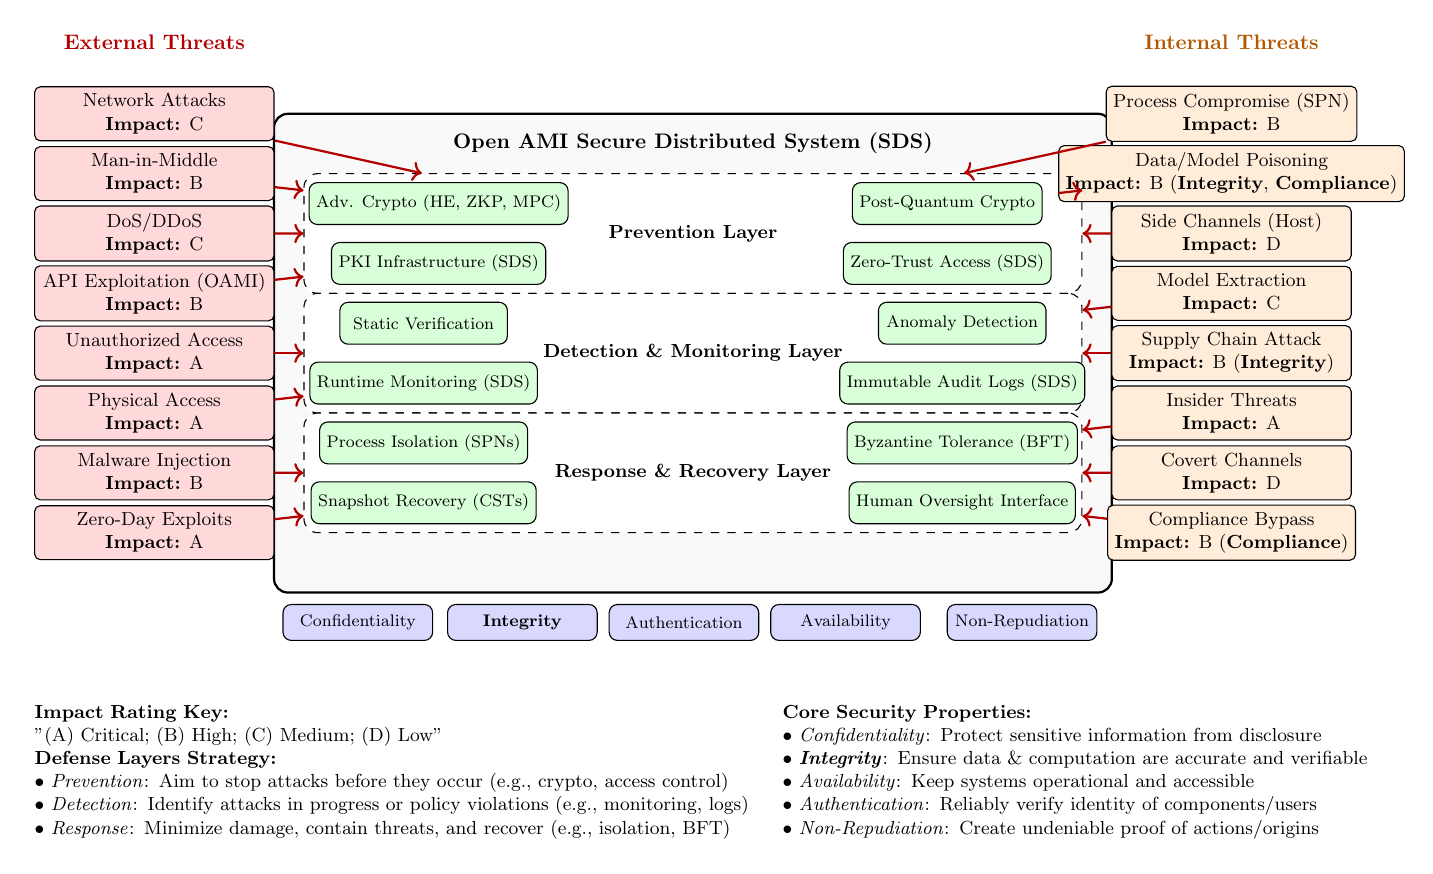
\begin{tikzpicture}[
			scale=0.76,
			transform shape,
			node distance=0.5cm,
			threat/.style={rectangle, rounded corners=2pt, draw=black, minimum width=2.8cm, minimum height=0.7cm, font=\footnotesize, align=center},
			external/.style={threat, fill=red!15},
			internal/.style={threat, fill=orange!15},
			defense/.style={rectangle, rounded corners=3pt, draw=black, fill=green!15, minimum width=2.8cm, minimum height=0.7cm, font=\footnotesize, align=center},
			property/.style={rectangle, rounded corners=3pt, draw=black, fill=blue!15, minimum width=2.5cm, minimum height=0.6cm, font=\footnotesize, align=center},
			system/.style={rectangle, rounded corners=5pt, draw=black, thick, fill=gray!5, minimum width=14cm, minimum height=8cm, align=center},
			layer/.style={rectangle, rounded corners=5pt, draw=black, dashed, fill=white, minimum width=13cm, minimum height=2cm, align=center, font=\small},
			impact/.style={circle, inner sep=0pt, font=\small},
			threatarrow/.style={->, thick, red!70!black},
			defensearrow/.style={->, thick, green!50!black},
			propertyarrow/.style={->, dashed, blue!70!black},
			note/.style={rectangle, draw=none, fill=none, align=left, font=\small}
			]
			
			% Main system container
			\node[system] (sds) at (0,0) {};
			\node[align=center] at (0,3.5) {\textbf{Open AMI Secure Distributed System (SDS)}};
			
			% Defense layers
			\node[layer] (prevention) at (0,2) {\textbf{Prevention Layer}};
			\node[layer] (detection) at (0,0) {\textbf{Detection \& Monitoring Layer}};
			\node[layer] (response) at (0,-2) {\textbf{Response \& Recovery Layer}};
			
			% EXTERNAL THREATS - Left side
			\node[external, align=center, minimum width=4cm, font=\small] (network) at (-9,4) {Network Attacks \\ \small{\textbf{Impact:} C}};
			\node[external, align=center, minimum width=4cm, font=\small] (mitm) at (-9,3) {Man-in-Middle \\ \small{\textbf{Impact:} B}};
			\node[external, align=center, minimum width=4cm, font=\small] (dos) at (-9,2) {DoS/DDoS \\ \small{\textbf{Impact:} C}};
			\node[external, align=center, minimum width=4cm, font=\small] (api) at (-9,1) {API Exploitation (OAMI) \\ \small{\textbf{Impact:} B}};
			\node[external, align=center, minimum width=4cm, font=\small] (access) at (-9,0) {Unauthorized Access \\ \small{\textbf{Impact:} A}};
			\node[external, align=center, minimum width=4cm, font=\small] (physical) at (-9,-1) {Physical Access \\ \small{\textbf{Impact:} A}};
			\node[external, align=center, minimum width=4cm, font=\small] (malware) at (-9,-2) {Malware Injection \\ \small{\textbf{Impact:} B}};
			\node[external, align=center, minimum width=4cm, font=\small] (zero) at (-9,-3) {Zero-Day Exploits \\ \small{\textbf{Impact:} A}};
			
			\node[text=red!70!black] at (-9,5.2) {\textbf{External Threats}};
			
			% INTERNAL THREATS - Right side
			\node[internal, align=center, minimum width=4cm, font=\small] (compromise) at (9,4) {Process Compromise (SPN) \\ \small{\textbf{Impact:} B}};
			\node[internal, align=center, minimum width=4cm, font=\small] (poison) at (9,3) {Data/Model Poisoning \\ \small{\textbf{Impact:} B (\Integrity, \textbf{Compliance})}};
			\node[internal, align=center, minimum width=4cm, font=\small] (side) at (9,2) {Side Channels (Host) \\ \small{\textbf{Impact:} D}};
			\node[internal, align=center, minimum width=4cm, font=\small] (inference) at (9,1) {Model Extraction \\ \small{\textbf{Impact:} C}};
			\node[internal, align=center, minimum width=4cm, font=\small] (supply) at (9,0) {Supply Chain Attack \\ \small{\textbf{Impact:} B (\Integrity)}};
			\node[internal, align=center, minimum width=4cm, font=\small] (insider) at (9,-1) {Insider Threats \\ \small{\textbf{Impact:} A}};
			\node[internal, align=center, minimum width=4cm, font=\small] (covert) at (9,-2) {Covert Channels \\ \small{\textbf{Impact:} D}};
			\node[internal, align=center, minimum width=4cm, font=\small] (compliance) at (9,-3) {Compliance Bypass \\ \small{\textbf{Impact:} B (\textbf{Compliance})}};
			
			\node[text=orange!70!black] at (9,5.2) {\textbf{Internal Threats}};
			
			% PREVENTION DEFENSES
			\node[defense] (crypto) at (-4.25,2.5) {Adv. Crypto (HE, ZKP, MPC)};
			\node[defense] (pki) at (-4.25,1.5) {PKI Infrastructure (SDS)};
			\node[defense] (postq) at (4.25,2.5) {Post-Quantum Crypto};
			\node[defense] (access_control) at (4.25,1.5) {Zero-Trust Access (SDS)};
			
			% DETECTION DEFENSES
			\node[defense] (static) at (-4.5,.5) {Static Verification};
			\node[defense] (runtime) at (-4.5,-.5) {Runtime Monitoring (SDS)};
			\node[defense] (anomaly) at (4.5,.5) {Anomaly Detection};
			\node[defense] (audit) at (4.5,-.5) {Immutable Audit Logs (SDS)};
			
			% RESPONSE DEFENSES
			\node[defense] (isolation) at (-4.5,-1.5) {Process Isolation (SPNs)};
			\node[defense] (recovery) at (-4.5,-2.5) {Snapshot Recovery (CSTs)};
			\node[defense] (redundancy) at (4.5,-1.5) {Byzantine Tolerance (BFT)};
			\node[defense] (human) at (4.5,-2.5) {Human Oversight Interface};
			
			% SECURITY PROPERTIES - Bottom
			\node[property] (conf) at (-5.6,-4.5) {Confidentiality};
			\node[property] (int_prop) at (-2.85,-4.5) {\Integrity};
			\node[property] (auth) at (-0.15,-4.5) {Authentication};
			\node[property] (avail) at (2.55,-4.5) {Availability};
			\node[property] (nonrep) at (5.5,-4.5) {Non-Repudiation};
			
			% Threat arrows - selective connections for clarity
			\draw[threatarrow] (network) -- (prevention);
			\draw[threatarrow] (mitm) -- (prevention);
			\draw[threatarrow] (dos) -- (prevention);
			\draw[threatarrow] (api) -- (prevention);
			\draw[threatarrow] (access) -- (detection);
			\draw[threatarrow] (physical) -- (detection);
			\draw[threatarrow] (malware) -- (response);
			\draw[threatarrow] (zero) -- (response);
			
			\draw[threatarrow] (compromise) -- (prevention);
			\draw[threatarrow] (poison) -- (prevention); % Threatens Integrity
			\draw[threatarrow] (side) -- (prevention);
			\draw[threatarrow] (inference) -- (detection);
			\draw[threatarrow] (supply) -- (detection); % Threatens Integrity
			\draw[threatarrow] (insider) -- (response);
			\draw[threatarrow] (covert) -- (response);
			\draw[threatarrow] (compliance) -- (response); % Threatens Compliance
			
			% Explanatory notes
			\node[note, text width=14cm, font=\small] at (-4,-7) {
				\textbf{Impact Rating Key:}
				\\ "(A) Critical; (B) High; (C) Medium; (D) Low"
				\\ \textbf{Defense Layers Strategy:}
				\\ $\bullet$ \textit{Prevention}: Aim to stop attacks before they occur (e.g., crypto, access control)
				\\ $\bullet$ \textit{Detection}: Identify attacks in progress or policy violations (e.g., monitoring, logs)
				\\ $\bullet$ \textit{Response}: Minimize damage, contain threats, and recover (e.g., isolation, BFT)
			};
			
			\node[note, text width=10cm, font=\small] at (6.5,-7) {
				\textbf{Core Security Properties:}
				\\ $\bullet$ \textit{Confidentiality}: Protect sensitive information from disclosure
				\\ $\bullet$ \textit{\Integrity}: Ensure data \& computation are accurate and verifiable
				\\ $\bullet$ \textit{Availability}: Keep systems operational and accessible
				\\ $\bullet$ \textit{Authentication}: Reliably verify identity of components/users
				\\ $\bullet$ \textit{Non-Repudiation}: Create undeniable proof of actions/origins
			};
			
		\end{tikzpicture}
		\caption[Open AMI SDS Threat Model and Defenses]{Open AMI SDS Threat Model and Defense Mechanisms. Illustrates key external and internal threats (with indicative impact ratings) targeting AI systems. Layered defenses (Prevention, Detection, Response) within the SDS aim to mitigate these threats and uphold core security properties. Threats specifically targeting system \Integrity\ (e.g., data/model poisoning, supply chain compromise) and \textbf{Compliance} mechanisms (e.g., bypass attempts) are central concerns addressed by the SDS design.}
		\label{fig:threat-model}
	\end{figure}
	
	The core objectives of the SDS, reflecting the integration of Open AMI's pillars, are:
	\begin{enumerate}[noitemsep]
		\item \textbf{Confidentiality}: Protect sensitive data (parameters, intermediate states, user data) from unauthorized disclosure, using encryption and access control enforced by SPNs and OAMI interfaces. TEEs can provide stronger guarantees \citep{Citadel_PlusPlus_2025}.
		\item \Integrity: Ensure the authenticity, verifiability, and reliable protection against unauthorized modification for all critical system elements: data, models, computations (training/inference), communications (OAMI), and logs. This is a cornerstone of the SDS, potentially proven via cryptographic methods \citep{Peng2025ZKMLSurvey, Jia2021ProofOfLearning}.
		\item \textbf{Availability}: Maintain system functionality and responsiveness, using redundancy (multiple SPNs), fault tolerance (BFT consensus), and state recovery (CSTs).
		\item \textbf{Authentication}: Reliably verify the identity of all communicating OAMI Components (SPNs, Meta-Processes, external interfaces) using cryptographic methods (e.g., mTLS certificates managed by the SDS PKI).
		\item \textbf{Authorization}: Enforce access controls based on verified identities and \textbf{Compliance} policies defined in the Compliance Manifest ($\mathcal{CM}$), applied to OAMI requests and resource access within SPNs.
		\item \textbf{Non-repudiation}: Create verifiable, tamper-evident records (leveraging SDS \Integrity\ mechanisms like signed logs and CSTs) of significant actions, decisions, state changes, and communications for audit and accountability, possibly using ledger technologies \citep{ProML_Provenance_2022}.
		\item \textbf{Compliance Enforcement}: Provide the underlying mechanisms (secure execution in SPNs, verified OAMI communication, state validation via CSTs) needed to enforce \textbf{Compliance} constraints (derived from $\mathcal{CM}$) on all operations, including ML processes, across relevant \Abstraction\ levels.
		\item \textbf{Auditability}: Enable comprehensive, secure logging (with guaranteed log \Integrity) by the SDS to support \textbf{Compliance} verification, security forensics, and analysis of system processes and \Dynamics.
		\item \textbf{Adaptive Dynamics Support}: Provide a stable yet flexible infrastructure capable of supporting adaptive learning and operation, including resource management (within SPNs/Hosts), monitoring of system \Dynamics\ (via OAMI reports), and controlled updates (verified by SDS mechanisms).
		\item \textbf{Transparency Support}: Offer interfaces (via OAMI) and mechanisms allowing higher layers (Governance, Intelligence) to inspect operational state and processes across different \Abstraction\ levels, while respecting \textbf{Compliance} rules (e.g., privacy during inspection).
	\end{enumerate}
	The SDS architecture implements these objectives through cryptographic techniques, process isolation (SPNs), runtime monitoring, secure protocols (OAMI), and specific architectural patterns detailed below.
	
	\section{Architectural Components and Integration} % Corrected Section Title and Numbering
	\label{sec:4-2} % Adjusted label
	
	The SDS provides the secure execution environment for all OAMI Components (which implement the system's logic, including AI/ML models).
	
	\subsection{Key Components and Definitions} % Corrected Section Title and Numbering
	\label{sec:4-2-1} % Adjusted label
	
	\begin{definition}[Secure Process Node (SPN)]
		\label{def:spn}
		An SPN is the fundamental unit of isolated execution within the SDS. It encapsulates an OAMI Component's logic (e.g., a specific ML model for inference, a training process, a data validation module, an ARU) defined as a Process $P$ (Def~\ref{def:compliant_process}) potentially operating at a specific \Abstraction\ level. Each SPN runs within a secure boundary (e.g., container, VM, TEE \citep{Citadel_PlusPlus_2025}) provided by the host infrastructure and managed by the SDS. It includes:
		\begin{itemize}[noitemsep]
			\item Process Logic $P$: The specific function or task performed by the component.
			\item Local State $S_n$: The internal state variables of the component.
			\item Local \textbf{Compliance} Enforcement Module $A_n$: Checks local actions/states against relevant constraints from $\mathcal{CM}$.
			\item \Integrity\ Module ($V_n, C_n, K_n$): Manages local cryptographic keys ($K_n$ provided/managed by SDS), performs cryptographic operations ($C_n$, e.g., signing CSTs, encrypting data, generating/verifying proofs \citep{Peng2025ZKMLSurvey}), and runs local \Integrity\ checks ($V_n$).
			\item Communication Interface: Implements the OAMI protocol (Appendix~\ref{app:protocol_spec}) for secure interaction with other components, managed by the SDS.
			\item Local \Dynamics\ Monitor $M_n^{\text{Dyn}}$: Tracks local resource usage, performance metrics, reports to Meta-Process/Governance via OAMI.
		\end{itemize}
		SPNs ensure that computations, including sensitive ML operations, occur in a controlled environment where \textbf{Compliance} can be enforced locally and computational \Integrity\ can be maintained and potentially verified by the SDS.
	\end{definition}
	
	\begin{definition}[Meta-Process]
		\label{def:meta_process}
		A Meta-Process is a specialized OAMI Component, typically running within its own SPN(s), responsible for coordinating, monitoring, and controlling a group of other SPNs ($\mathcal{N}_m$). Its functions include:
		\begin{itemize}[noitemsep]
			\item Enforcing cross-SPN or system-wide \textbf{Compliance} rules defined in $\mathcal{CM}$ (based on aggregated SPN reports).
			\item Aggregating \Integrity\ status reports from managed SPNs (received via OAMI), potentially verifying proofs.
			\item Managing collective system \Dynamics\ (e.g., coordinating updates, load balancing based on $M_n^{\text{Dyn}}$ reports).
			\item Operating at a higher \Abstraction\ level than the SPNs it manages.
			\item Interacting with its managed SPNs via the secure OAMI protocol.
			\item Potentially serving as an interface point for the Governance Layer or human oversight.
			\item Orchestrating distributed protocols like BFT consensus or secure aggregation, techniques common in privacy-preserving ML \citep{AdditionalCitationRef54}.
		\end{itemize}
		Meta-processes implement higher-level control and governance logic within the SDS.
	\end{definition}
	
	\begin{definition}[Cryptographic State Token (CST)]
		\label{def:cst_sds}
		A Cryptographic State Token (CST) is a secure, cryptographically signed (\Integrity-protected) summary or snapshot of an SPN's state $s_n(t)$ at a specific time $t$, generated by the SPN's \Integrity\ module $C_n$. It typically includes associated metadata such as a timestamp, \textbf{Compliance} status flags, the relevant \Abstraction\ level, and key \Dynamics\ indicators. CSTs are essential for:
		\begin{itemize}[noitemsep]
			\item Creating verifiable checkpoints of SPN states managed by the SDS.
			\item Enabling secure state synchronization between SPNs (see Algorithm~\ref{alg:secure_state_sync}).
			\item Providing tamper-evident records for auditing and non-repudiation stored in the SDS secure logs, potentially anchored to a ledger \citep{ProML_Provenance_2022}.
		\end{itemize}
		Formally, a CST might be generated as:
		\begin{align}
			\text{CST}_n(t) = \text{Sign}_{sk_n}(H(s_n(t) \| \text{metadata}(t))) \label{eq:cst_generation}
		\end{align}
		where $sk_n$ is the private signing key of SPN $n$ (managed securely by SDS), $H$ is a cryptographic hash function, and `metadata(t)` includes timestamp, compliance flags, etc. Verification uses the corresponding public key $pk_n$ obtained from the SDS PKI.
	\end{definition}
	
	\begin{definition}[Compliance Manifest ($\mathcal{CM}$) (Reference)]
		\label{def:cm_ref}
		As detailed in Chapter~\ref{ch:compliance}, the Compliance Manifest ($\mathcal{CM}$) is the authoritative, formal specification of all \textbf{Compliance} requirements (ethical, legal, operational, safety) governing the Open AMI system. Within the SDS, local checkers ($A_n$ in SPNs) and Meta-Processes use relevant parts of $\mathcal{CM}$ (securely distributed and integrity-verified) to guide verification and enforcement.
	\end{definition}
	
	Figure~\ref{fig:sds-architecture} illustrates how these components integrate within the SDS architecture. SPNs execute the core processes, are coordinated by Meta-Processes which enforce system-wide \textbf{Compliance} and manage overall \Dynamics, utilize CSTs to ensure state \Integrity, and communicate securely using the OAMI protocol over the underlying SDS infrastructure.
	
	\begin{figure}[ht]
		\centering
		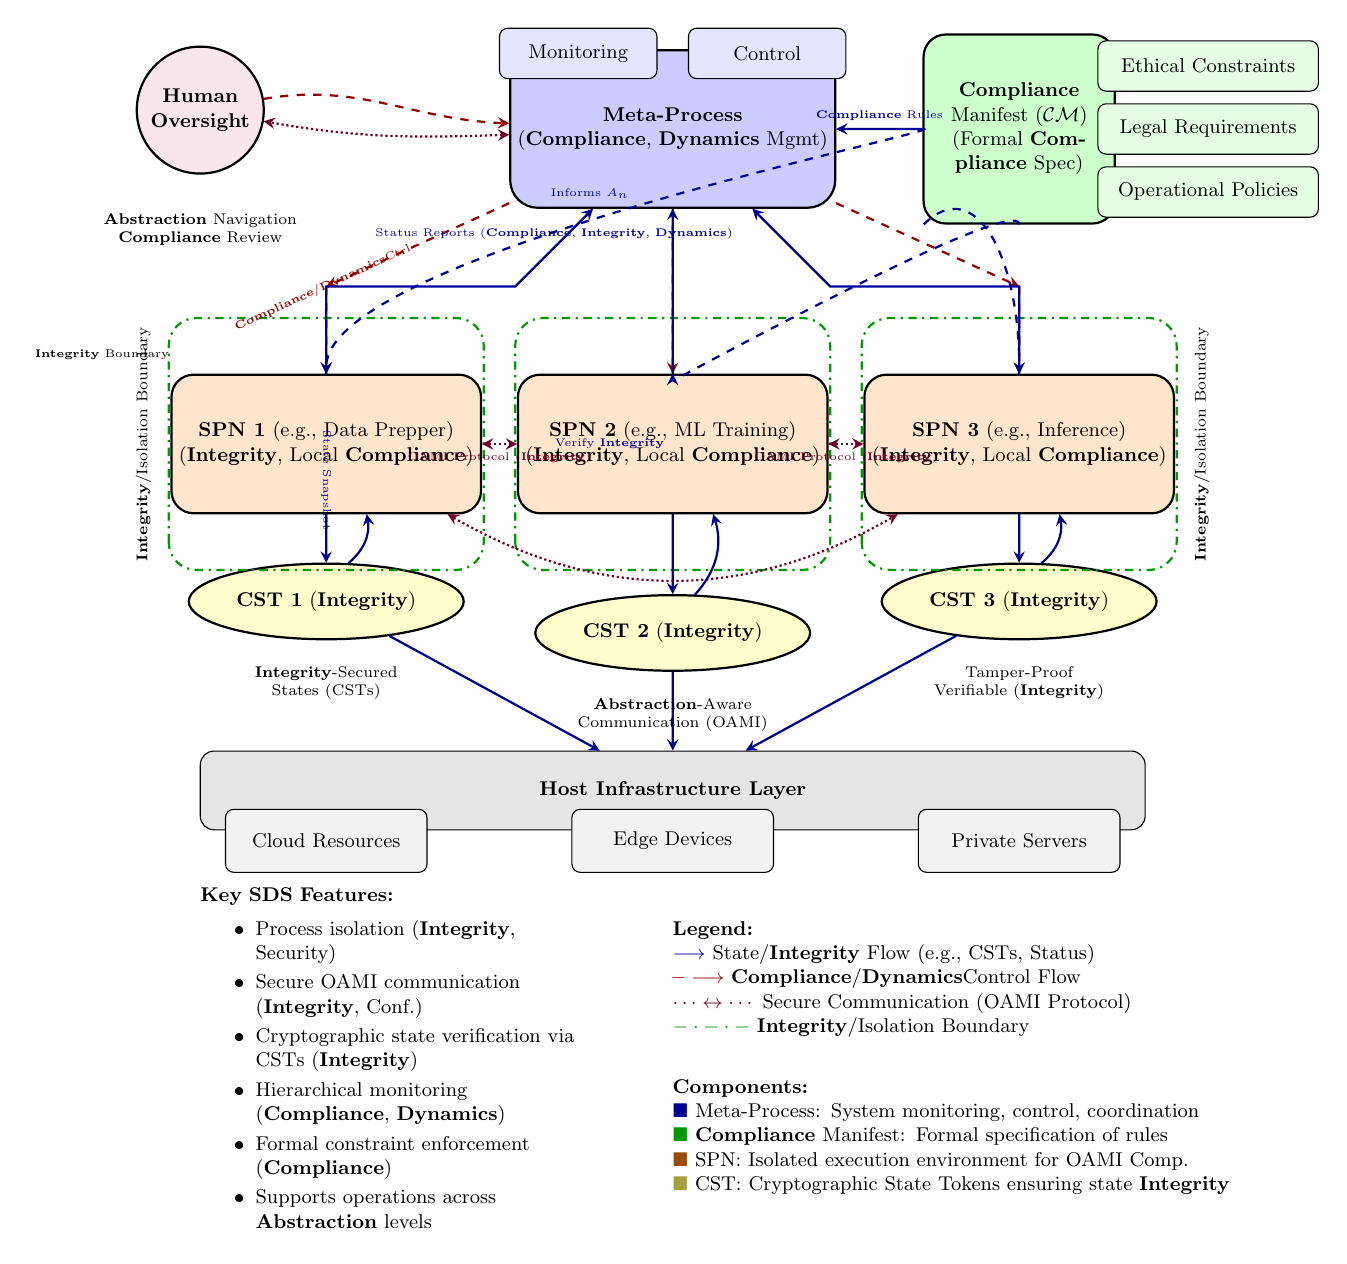
\begin{tikzpicture}[
			scale=0.8,
			transform shape,
			node distance=1cm,
			metaprocess/.style={rectangle, rounded corners=10pt, draw=black, thick, fill=blue!20, minimum width=5cm, minimum height=2.5cm, align=center, font=\small},
			metabox/.style={rectangle, rounded corners=3pt, draw=black, fill=blue!10, minimum width=2.5cm, minimum height=0.8cm, font=\small, align=center},
			spn/.style={rectangle, rounded corners=8pt, draw=black, thick, fill=orange!20, minimum width=4.2cm, minimum height=2.2cm, align=center, font=\small},
			spnbox/.style={rectangle, rounded corners=3pt, draw=black, fill=orange!10, minimum width=2cm, minimum height=0.5cm, font=\small, align=center},
			cst/.style={ellipse, draw=black, thick, fill=yellow!20, minimum width=2.5cm, minimum height=1.2cm, align=center, font=\small},
			manifest/.style={rectangle, rounded corners=8pt, draw=black, thick, fill=green!20, minimum width=3cm, minimum height=3cm, align=center, font=\small, text width=2.8cm},
			human/.style={circle, draw=black, thick, fill=purple!10, minimum size=2cm, font=\small, align=center},
			manifestbox/.style={rectangle, rounded corners=3pt, draw=black, fill=green!10, minimum width=3.5cm, minimum height=0.8cm, font=\small, align=center},
			infra/.style={rectangle, rounded corners=5pt, draw=black, fill=gray!20, minimum width=15cm, minimum height=1.25cm, align=center, font=\small},
			infrabox/.style={rectangle, rounded corners=3pt, draw=black, fill=gray!10, minimum width=3.2cm, minimum height=1cm, font=\small, align=center},
			dataflow/.style={->, >=stealth, thick, blue!60!black},
			controlflow/.style={->, >=stealth, thick, red!60!black, dashed},
			securecomm/.style={<->, >=stealth, thick, purple!60!black, densely dotted},
			security/.style={thick, dashdotted, green!60!black},
			note/.style={rectangle, draw=none, fill=white!90, align=left, font=\small, rounded corners=2pt},
			legend/.style={rectangle, draw=none, align=left, font=\small},
			nodelabel/.style={align=center, font=\scriptsize}
			]
			
			\node[human] (human) at (-7.5,5.3) {\textbf{Human}\\{\textbf{Oversight}}};
			\node[nodelabel] at (-7.5,3.4) {\Abstraction\ Navigation\\\textbf{Compliance} Review};
			
			% Top Level - Meta-Process and Compliance Manifest
			\node[metaprocess] (meta) at (0,5) {\textbf{Meta-Process}\\(\textbf{Compliance}, \Dynamics\ Mgmt)};
			\node[metabox] (monitor) at (-1.5,6.2) {Monitoring};
			\node[metabox] (control) at (1.5,6.2) {Control};
			
			\node[manifest] (manifest) at (5.5,5) {\textbf{\Compliance} Manifest ($\mathcal{CM}$)\\(Formal \textbf{Compliance} Spec)};
			\node[manifestbox] (ethical) at (8.5,6) {Ethical Constraints};
			\node[manifestbox] (legal) at (8.5,5) {Legal Requirements};
			\node[manifestbox] (ops) at (8.5,4) {Operational Policies};
			
			% Mid Level - Secure Process Nodes (with more space between them)
			\node[spn] (spn1) at (-5.5,0) {\textbf{SPN 1} (e.g., Data Prepper)\\(\Integrity, Local \textbf{Compliance})};
			\node[spn] (spn2) at (0,0) {\textbf{SPN 2} (e.g., ML Training)\\(\Integrity, Local \textbf{Compliance})};
			\node[spn] (spn3) at (5.5,0) {\textbf{SPN 3} (e.g., Inference)\\(\Integrity, Local \textbf{Compliance})};
			
			% Cryptographic State Tokens
			\node[cst] (cst1) at (-5.5,-2.5) {\textbf{CST 1} (\Integrity)};
			\node[cst] (cst2) at (0,-3) {\textbf{CST 2} (\Integrity)};
			\node[cst] (cst3) at (5.5,-2.5) {\textbf{CST 3} (\Integrity)};
			
			% Bottom Level - Host Infrastructure (more space below)
			\node[infra] (infra) at (0,-5.5) {\textbf{Host Infrastructure Layer}};
			\node[infrabox] (cloud) at (-5.5,-6.3) {Cloud Resources};
			\node[infrabox] (edge) at (0,-6.3) {Edge Devices};
			\node[infrabox] (private) at (5.5,-6.3) {Private Servers};
			
			% Human oversight connections
			\draw[securecomm, thick] (meta) to[out=182,in=350] (human);
			\draw[controlflow, thick] (human) to[out=10,in=178] (meta);
			
			% Security/Integrity boundaries
			\draw[security, rounded corners=10pt] (-8.0,-2.0) rectangle (-3.0,2.0); % SPN 1 boundary
			\node [above left=0.1cm and -0.1cm of spn1.north west, align=center, font=\tiny] {\Integrity\ Boundary};
			\draw[security, rounded corners=10pt] (-2.5,-2.0) rectangle (2.5,2.0); % SPN 2 boundary
			\draw[security, rounded corners=10pt] (3.0,-2.0) rectangle (8.0,2.0); % SPN 3 boundary
			
			
			% Control signals - MetaProcess to SPNs
			\draw[controlflow] (meta) -- (-5.5,2.5) node[midway, left, sloped, font=\tiny] {\textbf{Compliance}/\Dynamics Ctrl};
			\draw[controlflow] (-5.5,2.5) -- (spn1);
			\draw[controlflow] (meta) -- (spn2);
			\draw[controlflow] (meta) -- (5.5,2.5);
			\draw[controlflow] (5.5,2.5) -- (spn3);
			
			% Compliance Manifest to Meta Process / SPNs (Conceptually informs A_n)
			\draw[dataflow] (manifest) -- (meta) node[midway, above, font=\tiny] {\textbf{Compliance} Rules};
			\draw[dataflow, dashed] (manifest) .. controls +(west:1) and +(north:3) .. (spn1) node[midway, above left, font=\tiny] {Informs $A_n$};
			\draw[dataflow, dashed] (manifest) .. controls +(south:1) and +(north:1) .. (spn2);
			\draw[dataflow, dashed] (manifest) .. controls +(south west:1) and +(north:3) .. (spn3);
			
			
			% SPNs to CSTs (State with Integrity)
			\draw[dataflow] (spn1) -- (cst1) node[midway, left, sloped, font=\tiny] {State Snapshot};
			\draw[dataflow] (spn2) -- (cst2);
			\draw[dataflow] (spn3) -- (cst3);
			
			% CSTs to Infrastructure (Persistence)
			\draw[dataflow] (cst1) -- (infra);
			\draw[dataflow] (cst2) -- (infra);
			\draw[dataflow] (cst3) -- (infra);
			
			% Secure communications between SPNs (OAMI Protocol)
			\draw[securecomm] (spn1) -- (spn2) node[midway, below, font=\tiny] {OAMI Protocol (\Integrity)};
			\draw[securecomm] (spn2) -- (spn3) node[midway, below, font=\tiny] {OAMI Protocol (\Integrity)};
			\draw[securecomm, bend right=30] (spn1) to (spn3);
			
			% CST verification loops (Integrity Check)
			\draw[dataflow, ->, >=stealth, bend right=30] (cst1) to (spn1) node[midway, left, sloped, font=\tiny] {Verify \Integrity};
			\draw[dataflow, ->, >=stealth, bend right=30] (cst2) to (spn2);
			\draw[dataflow, ->, >=stealth, bend right=30] (cst3) to (spn3);
			
			% Verification flows from SPNs to MetaProcess (Compliance/Integrity/Dynamics Status)
			\draw[dataflow, ->, >=stealth] (spn1) -- (-5.5,2.5) -- (-2.5,2.5) -- (meta) node[midway, above, font=\tiny] {Status Reports (\textbf{Compliance}, \Integrity, \Dynamics)};
			\draw[dataflow, ->, >=stealth] (spn2) -- (meta);
			\draw[dataflow, ->, >=stealth] (spn3) -- (5.5,2.5) -- (2.5,2.5) -- (meta);
			
			% Annotations
			\node[nodelabel] at (-5.5,-3.8) {\Integrity-Secured\\States (CSTs)};
			\node[nodelabel] at (0,-4.3) {\Abstraction-Aware\\Communication (OAMI)};
			\node[nodelabel] at (5.5,-3.8) {Tamper-Proof\\Verifiable (\Integrity)};
			
			\node[nodelabel, rotate=90] at (-8.4,0) {\Integrity/Isolation Boundary};
			\node[nodelabel, rotate=90] at (8.4,0) {\Integrity/Isolation Boundary};
			
			% Legend elements arranged vertically (moved down)
			\node[legend, text width=10cm, align=left, fill=white] at (5,-8.5) {
				\textbf{Legend:}\\
				\textcolor{blue!60!black}{$\longrightarrow$} State/\Integrity\ Flow (e.g., CSTs, Status)\\
				\textcolor{red!60!black}{\textbf{-- $\longrightarrow$}} \textbf{Compliance}/\Dynamics Control Flow\\
				\textcolor{purple!60!black}{$\cdots\leftrightarrow\cdots$} Secure Communication (OAMI Protocol)\\
				\textcolor{green!60!black}{$\mathbf{- \cdot - \cdot -}$} \Integrity/Isolation Boundary
			};
			
			% Components list arranged vertically (moved down)
			\node[legend, text width=10cm, align=left, fill=white] at (5,-11) {
				\textbf{Components:}\\
				\textcolor{blue!60!black}{$\blacksquare$} Meta-Process: System monitoring, control, coordination\\
				\textcolor{green!60!black}{$\blacksquare$} \textbf{Compliance} Manifest: Formal specification of rules\\
				\textcolor{orange!60!black}{$\blacksquare$} SPN: Isolated execution environment for OAMI Comp.\\
				\textcolor{yellow!60!black}{$\blacksquare$} CST: Cryptographic State Tokens ensuring state \Integrity\
			};
			
			% Key features callouts (improved box, moved to bottom left, adjusted position)
			\node[note, text width=6cm] at (-4.5,-9.75) {
				\textbf{Key SDS Features:}
				\begin{itemize}[itemsep=.01cm]
					\item Process isolation (\Integrity, Security)
					\item Secure OAMI communication (\Integrity, Conf.)
					\item Cryptographic state verification via CSTs (\Integrity)
					\item Hierarchical monitoring (\textbf{Compliance}, \Dynamics)
					\item Formal constraint enforcement (\textbf{Compliance})
					\item Supports operations across \Abstraction\ levels
				\end{itemize}
			};
			
		\end{tikzpicture}
		\caption[Open AMI SDS Architecture]{Open AMI Secure Distributed System Architecture. Secure Process Nodes (SPNs) provide isolated execution environments for OAMI Components, ensuring local \Integrity\ and \textbf{Compliance} checks. Meta-Processes coordinate SPNs, enforce system-wide \textbf{Compliance}, and manage collective \Dynamics. Cryptographic State Tokens (CSTs) guarantee state \Integrity. Secure communication uses the OAMI protocol. Human oversight interacts via designated interfaces, enabling \Abstraction\ navigation and \textbf{Compliance} review.}
		\label{fig:sds-architecture}
	\end{figure}
	
	\subsection{Integration with Theoretical Framework} % Corrected Section Title and Numbering
	\label{sec:4-2-2} % Adjusted label
	
	The SDS architecture directly implements the theoretical principles discussed in Chapter~\ref{ch:theoretical_framework}:
	\begin{enumerate}[noitemsep]
		\item \textbf{Process Theory:} SPNs serve as the execution containers for formally defined processes (Def~\ref{def:compliant_process}), enforcing their \textbf{Compliance} and \Integrity\ invariants (Eq.~\ref{eq:proc_comp}, \ref{eq:proc_int}). Meta-Processes manage process interactions (Def~\ref{def:compliant_interaction}) via OAMI and collective \Dynamics.
		\item \textbf{Cognitive Mapping:} Meta-Processes may utilize knowledge structures (Def~\ref{def:knowledge_category}), potentially hosted in dedicated SPNs accessible via OAMI \texttt{knowledge/} methods, representing relationships across different \Abstraction\ levels for coordination. Knowledge \Integrity\ (Def~\ref{def:knowledge_integrity}) is maintained by the hosting SPN and SDS mechanisms.
		\item \textbf{Atomic Reasoning:} SPNs provide the verifiable (\Integrity) and isolated execution environment required for ARUs (Def~\ref{def:aru}). The SDS ensures the integrity of ARU composition via secure OAMI communication (Theorem~\ref{thm:aru_integrity_composition}). Physics-inspired ARUs leverage OASIM simulation capabilities executed within or securely accessed by SPNs via OAMI.
		\item \textbf{Compliant Learning:} SPNs host ML training and inference processes (Chapter~\ref{ch:machine_learning}), providing the secure environment needed to enforce data \textbf{Compliance}, ensure algorithmic \Integrity\ (potentially via PoL/ZKPs), securely handle model artifacts, and manage learning \Dynamics\ according to Def~\ref{def:compliant_learning}.
		\item \textbf{Guidance Functions:} Meta-Processes issue guidance commands (Def~\ref{def:guidance_function}) to SPNs via the secure OAMI protocol, steering the system while maintaining system-wide \textbf{Compliance} and \Integrity.
		\item \textbf{Operational Self-Awareness:} principles (Sec~\ref{sec:2-11}) inform the monitoring functions within the Governance Layer, tracking \textbf{Compliance} status, \Integrity, \Abstraction\ usage, and system \Dynamics\ based on data aggregated from the SDS.
	\end{enumerate}
	This tight integration ensures that the SDS provides a trustworthy operational foundation consistent with the framework's theoretical guarantees.
	
	\subsection{Host Infrastructure Requirements and SPN Implementation} % Corrected Section Title and Numbering
	\label{sec:4-2-3} % Adjusted label
	
	Effective operation of the SDS relies on certain capabilities provided by the underlying host infrastructure and choices made in implementing SPNs:
	
	\subsubsection{Host Infrastructure Requirements} % Corrected Section Title and Numbering
	\label{sec:4-2-3-1} % Adjusted label for subsection
	\begin{enumerate}[noitemsep]
		\item \textbf{Isolation Mechanisms:} Secure execution environments are fundamental for SPN security and \Integrity\ isolation. Options include Containers (e.g., Docker, Kubernetes Pods with security contexts), Virtual Machines (VMs), or Hardware-based Trusted Execution Environments (TEEs) like Intel SGX or AMD SEV, as used in systems like Citadel++ \citep{Citadel_PlusPlus_2025}.
		\item \textbf{Cryptographic Acceleration:} Hardware support for cryptographic primitives (e.g., AES-NI, SHA extensions) is crucial for acceptable performance of SDS \Integrity\ mechanisms.
		\item \textbf{Secure Communication Channels:} Reliable and secure network infrastructure supporting protocols like TLS 1.3 with mutual authentication (mTLS) is required for OAMI.
		\item \textbf{Resource Monitoring:} Capabilities for monitoring CPU, memory, network, and potentially energy usage are needed for managing system \Dynamics\ and detecting certain anomalies.
		\item \textbf{Platform Integrity Verification (Optional but Recommended):} Mechanisms like Secure Boot and Remote Attestation allow verification of the host platform's integrity, providing a stronger root of trust for the SDS and the SPNs running on it, especially important when using TEEs \citep{Citadel_PlusPlus_2025}.
	\end{enumerate}
	
	\subsubsection{SPN Implementation Considerations} % Corrected Section Title and Numbering
	\label{sec:4-2-3-2} % Adjusted label for subsection
	The choice of isolation technology for SPNs impacts the level of \Integrity\ assurance and performance:
	\begin{itemize}
		\item \textbf{Containers:} Offer lightweight isolation, good performance, and ease of deployment. Rely heavily on the host OS kernel security. Suitable for many applications where host compromise is considered less likely or where defense-in-depth is sufficient. Provide process-level isolation.
		\item \textbf{Virtual Machines (VMs):} Provide stronger isolation by virtualizing hardware and running a separate OS kernel. Offer better protection against host OS compromise but incur higher performance overhead than containers.
		\item \textbf{Trusted Execution Environments (TEEs):} Offer the strongest hardware-enforced isolation for code and data confidentiality and \Integrity, even from a compromised host OS or hypervisor \citep{Citadel_PlusPlus_2025}. Provide runtime attestation capabilities, allowing remote verification of the SPN's software state. Incur performance overhead, have memory limitations, and require specific hardware support. Ideal for highly sensitive computations or ensuring the \Integrity\ of critical compliance checks.
	\end{itemize}
	The specific SPN implementation choice should be based on a risk assessment considering the sensitivity of the process running within the SPN, the trust level of the host infrastructure, and performance requirements, potentially defined as a \textbf{Compliance} requirement in $\mathcal{CM}$.
	
	\section{Cryptographic Foundations and Integrity Mechanisms} % Corrected Section Title and Numbering
	\label{sec:4-3} % Adjusted label
	
	Cryptography is the bedrock of the \Integrity, confidentiality, and authenticity guarantees provided by the SDS.
	
	\subsection{Cryptographic Building Blocks} % Corrected Section Title and Numbering
	\label{sec:4-3-1} % Adjusted label
	
	The SDS utilizes standard, well-vetted cryptographic primitives, typically executed within SPN \Integrity\ modules or dedicated SDS services:
	\begin{itemize}[noitemsep]
		\item \textbf{Symmetric Encryption:} AES (e.g., AES-GCM) for protecting OAMI data in transit (within TLS) and potentially data at rest within SPNs or storage managed by SDS. $c = \text{Enc}_K(m), m = \text{Dec}_K(c)$.
		\item \textbf{Asymmetric Encryption:} RSA or ECC for key exchange (TLS handshake).
		\item \textbf{Digital Signatures:} ECDSA or EdDSA for verifying authenticity and \Integrity\ of OAMI messages (optional payload signing), code/models deployed to SPNs, CSTs, and logs. $\sigma = \text{Sign}_{sk}(m), \text{Verify}_{pk}(m, \sigma) \in \{\text{true}, \text{false}\}$. Keys managed by SDS PKI.
		\item \textbf{Hash Functions:} SHA-256 or SHA-3 for creating digests to verify data \Integrity\ (e.g., within CSTs, logs). $h = H(m)$.
		\item \textbf{Message Authentication Codes (MACs):} Used within TLS (e.g., HMAC) to ensure message \Integrity\ and authenticity over secure channels. $t = \text{MAC}_K(m), \text{Verify}_K(m, t) \in \{\text{true}, \text{false}\}$.
	\end{itemize}
	These primitives are essential for securing OAMI communications, protecting stored data and models, generating and verifying CSTs (\Integrity), and building secure audit trails.
	
	\subsection{Advanced Cryptographic Techniques} % Corrected Section Title and Numbering
	\label{sec:4-3-2} % Adjusted label
	
	Where necessary for enhanced privacy (\textbf{Compliance}) or verification (\Integrity), the SDS architecture supports the use of advanced cryptographic techniques, potentially implemented within specialized SPNs or libraries:
	\begin{itemize}[noitemsep]
		\item \textbf{Homomorphic Encryption (HE):} Allows computation (e.g., aggregation in Federated Learning) on encrypted data. Useful for privacy-preserving analytics. Performance is a major consideration.
		\item \textbf{Secure Multi-Party Computation (MPC):} Enables multiple SPNs to jointly compute a function over their private inputs without revealing them, as commonly used in privacy-preserving federated learning \citep{AdditionalCitationRef54}. Essential for complex collaborative tasks like privacy-preserving FL or joint analysis. Ensures process \Integrity\ and input confidentiality. Requires significant communication overhead, managed via OAMI coordination.
		\item \textbf{Zero-Knowledge Proofs (ZKPs):} Allow an SPN to prove the correctness of its computation (e.g., "I correctly executed this ML training step according to spec", "This update adheres to DP budget") without revealing internal state \citep{Peng2025ZKMLSurvey}. Powerful for verifiable computation (\Integrity) and private compliance verification (\textbf{Compliance}). $\text{Prove}(x, w) \rightarrow \pi, \text{Verify}(x, \pi) \in \{\text{true}, \text{false}\}$. Verification might be done by receiving SPN or Meta-Process. Proof-of-Learning \citep{Jia2021ProofOfLearning} is a related concept for verifying training.
		\item \textbf{Post-Quantum Cryptography (PQC):} Incorporates algorithms resistant to quantum attacks, ensuring long-term \Integrity\ and confidentiality. SDS PKI and OAMI TLS configurations should support PQC algorithms where required by policy ($\mathcal{CM}$).
	\end{itemize}
	The choice depends on specific security/\textbf{Compliance} requirements, performance constraints, and technology maturity. Open AMI provides the framework (SPNs, OAMI) to integrate these techniques where needed.
	
	\subsection{Cryptographic Protocol Suite for Integrity} % Corrected Section Title and Numbering
	\label{sec:4-3-3} % Adjusted label
	
	The SDS implements specific protocols, largely defined by the OAMI standard (Appendix~\ref{app:protocol_spec}), leveraging cryptographic blocks to ensure secure and integral interactions.
	
	\subsubsection{Secure Channel Establishment (OAMI/TLS)} % Corrected Section Title and Numbering
	\label{sec:4-3-3-1} % Adjusted label for subsubsection
	All OAMI communication MUST occur over secure channels established using TLS 1.3 (or comparable), requiring mutual authentication (mTLS) using certificates managed by the SDS PKI. This provides confidentiality, message \Integrity, and endpoint authentication.
	
	\subsubsection{Secure State Synchronization (CST-based)} % Corrected Section Title and Numbering
	\label{sec:4-3-3-2} % Adjusted label for subsubsection
	Cryptographic State Tokens (CSTs, Def~\ref{def:cst_sds}), generated by SPNs, are used for communicating verifiable state updates or checkpoints via OAMI messages. Algorithm~\ref{alg:secure_state_sync} outlines the basic verification process ensuring the \Integrity\ and authenticity of the received state.
	
	\begin{algorithm}[H]
		\caption{Secure State Synchronization Protocol (\Integrity\ Focus)}
		\label{alg:secure_state_sync}
		\begin{algorithmic}[1]
			\Require SPN $A$ intends to share state update $s_{A, \text{new}}$ (or snapshot) with SPN $B$.
			\State SPN $A$ generates relevant metadata $m_A$ (timestamp, seq number, compliance status, etc.).
			\State SPN $A$ computes hash $h = H(s_{A, \text{new}} \| m_A)$. \Comment{Bind state and metadata}
			\State SPN $A$ creates CST using its private key $sk_A$: $\text{CST}_A = \text{Sign}_{sk_A}(h)$. \Comment{Ensures \Integrity\ \& Authenticity}
			\State SPN $A$ sends $(s_{A, \text{new}}, m_A, \text{CST}_A)$ to SPN $B$ via secure OAMI channel.
			\State SPN $B$ receives the message.
			\State SPN $B$ computes the hash of the received state and metadata: $h' = H(s_{A, \text{new}} \| m_A)$.
			\State SPN $B$ retrieves $A$'s public key $pk_A$ (from SDS PKI).
			\State SPN $B$ verifies the signature: $result = \text{Verify}_{pk_A}(\text{CST}_A, h')$. \Comment{\Integrity\ \& Authenticity check}
			\If{$result$ is true}
			\State SPN $B$ accepts the state update $s_{A, \text{new}}$.
			\State (Optional) SPN $B$ may perform further validation based on $m_A$ (e.g., check \textbf{Compliance} status).
			\Else
			\State SPN $B$ rejects the update.
			\State SPN $B$ logs the \Integrity\ failure event (via SDS logging).
			\State SPN $B$ may notify Meta-Process or take other defensive actions via OAMI.
			\EndIf
		\end{algorithmic}
	\end{algorithm}
	
	\subsubsection{Secure Multi-Party Consensus (BFT)} % Corrected Section Title and Numbering
	\label{sec:4-3-3-3} % Adjusted label for subsubsection
	For critical operations requiring agreement among multiple SPNs or Meta-Processes (e.g., committing a global FL model, agreeing on a $\mathcal{CM}$ update), the SDS employs Byzantine Fault Tolerant (BFT) consensus protocols, orchestrated via OAMI messages. These ensure agreement on valid (\Integrity-preserving and \textbf{Compliant}) outcomes despite potential failures or malicious actors up to a certain threshold \citep{Karimireddy2021Byzantine}. Algorithm~\ref{alg:bft_consensus} provides a conceptual outline.
	
	\begin{algorithm}[H]
		\caption{Simplified BFT Consensus Protocol (\textbf{Compliance}/\Integrity\ Focus)}
		\label{alg:bft_consensus}
		\begin{algorithmic}[1]
			\Require Set of participating nodes $\mathcal{N}$ (SPNs/Meta-Processes), proposal $P$ with evidence $E_P$, max faulty nodes $f$, where $|\mathcal{N}| \ge 3f+1$. Nodes communicate via OAMI.
			\State A designated leader node proposes $(P, E_P)$ via OAMI messages.
			\ForAll{node $i \in \mathcal{N}$}
			\State Upon receiving proposal, verify proposal \Integrity\ (e.g., signature, format via OAMI checks) and \textbf{Compliance} (using local checker $A_i$ and $\mathcal{CM}$).
			\If{proposal is valid and compliant}
			\State Broadcast signed "PREPARE" message for $P$ via OAMI.
			\EndIf
			\EndFor
			\ForAll{node $i \in \mathcal{N}$}
			\If{node $i$ receives $2f+1$ valid PREPARE OAMI messages (verified for \Integrity) from distinct nodes for $P$}
			\State Broadcast signed "COMMIT" message for $P$ via OAMI.
			\State Mark $P$ as prepared locally.
			\EndIf
			\EndFor
			\ForAll{node $i \in \mathcal{N}$}
			\If{node $i$ receives $2f+1$ valid COMMIT OAMI messages (verified for \Integrity) from distinct nodes for $P$}
			\State Accept $P$ as the committed consensus decision. \Comment{Guarantees \Integrity\ \& \textbf{Compliance}}
			\State Execute or record $P$ locally. Log commitment via SDS logging.
			\State \textbf{return} $P$
			\EndIf
			\EndFor
			\State \Comment{If no proposal reaches commit after timeout, leader rotation or recovery may occur.}
			\State Log failure event via SDS logging.
			\State \textbf{return} Failure (or trigger recovery)
		\end{algorithmic}
	\end{algorithm}
	
	\section{Formal Verification and Trustworthiness Guarantees} % Corrected Section Title and Numbering
	\label{sec:4-4} % Adjusted label
	
	The SDS architecture is designed to support formal verification techniques, enabling provable guarantees about its security and trustworthiness properties (\Integrity, \textbf{Compliance}) under certain assumptions about the underlying components and host infrastructure.
	
	\subsection{Formal Properties (\textbf{Compliance} and \Integrity\ Focus)} % Corrected Section Title and Numbering
	\label{sec:4-4-1} % Adjusted label
	
	Formal verification efforts within the SDS aim to mathematically prove properties such as:
	\begin{itemize}[noitemsep]
		\item \textbf{Confidentiality}: Sensitive data within SPNs or OAMI messages is protected from unauthorized disclosure (via encryption, TEEs \citep{Citadel_PlusPlus_2025}).
		\item \textbf{Integrity (Data, Computation, Models, Logs)}: Critical system elements are protected from undetected modification (via hashing, signatures, verifiable computation \citep{Peng2025ZKMLSurvey}, secure logs \citep{ProML_Provenance_2022}).
		\item \textbf{Availability}: Essential services remain operational despite bounded failures (via redundancy, BFT).
		\item \textbf{Authentication}: Only legitimate components participate in OAMI communications (via mTLS, tokens).
		\item \textbf{Authorization}: Access controls based on identity and $\mathcal{CM}$ policies are correctly enforced for OAMI requests and SPN actions.
		\item \textbf{Non-repudiation}: Actions can be cryptographically attributed to originating SPNs (via signed logs, CSTs).
		\item \textbf{Compliance Adherence}: Operations executed within SPNs and coordinated by Meta-Processes adhere to $\mathcal{CM}$ constraints.
	\end{itemize}
	
	\subsection{Verification Mechanisms} % Corrected Section Title and Numbering
	\label{sec:4-4-2} % Adjusted label
	
	The SDS leverages multiple verification mechanisms:
	\begin{itemize}[noitemsep]
		\item \textbf{Static Analysis \& Verification:} Analyzing SPN code/configurations against security rules and \textbf{Compliance} constraints derived from $\mathcal{CM}$ before deployment. Ensures baseline \Integrity\ and \textbf{Compliance}.
		\item \textbf{Runtime Verification \& Monitoring:} Continuously monitoring SPN execution and OAMI interactions against \textbf{Compliance} rules (via $A_n$ checkers, Meta-Processes), verifying \Integrity\ (CSTs, OAMI checks), monitoring \Dynamics, using the SDS monitoring infrastructure.
		\item \textbf{Model Checking:} Analyzing abstract models of SDS protocols (consensus, synchronization) and interactions to verify system-level \Integrity\ and \textbf{Compliance} properties.
		\item \textbf{Runtime Attestation (with TEEs):} If SPNs use TEEs \citep{Citadel_PlusPlus_2025}, remote attestation can verify the software state and execution \Integrity\ to other components or the Governance Layer.
		\item \textbf{Cryptographic Proof Verification:} Verifying ZKPs \citep{Peng2025ZKMLSurvey} or PoL proofs \citep{Jia2021ProofOfLearning} generated by SPNs to attest to computation correctness or properties.
	\end{itemize}
	
	\subsection{Theorems and Proofs (Illustrative)} % Corrected Section Title and Numbering
	\label{sec:4-4-3} % Adjusted label
	
	Formal verification aims to establish theorems providing rigorous guarantees about the SDS.
	
	\begin{theorem}[Security Composition of SPNs]
		\label{thm:spn_composition_security}
		If individual SPNs $n_1, \dots, n_k$ are correctly implemented (potentially verified via static analysis/attestation) to satisfy local security/\textbf{Compliance} invariants ($\mathcal{I}_{n_i}^{\text{Int}}, \mathcal{I}_{n_i}^{\text{Comp}}$ from $\mathcal{CM}$), and interact solely through the verified OAMI protocol suite over secure channels provided by SDS, then the composed system maintains specified end-to-end security and \textbf{Compliance} properties, subject to assumptions about host infrastructure \Integrity\ and OAMI verification correctness.
	\end{theorem}
	\begin{proof} (Sketch) Induction on interactions, showing invariants preserved by SPN local checks and secure OAMI transfers enforced by SDS. Deferred to Appendix~\ref{app:proof_spn_composition}. \end{proof}
	
	\begin{theorem}[BFT Integrity and Compliance]
		\label{thm:bft_integrity_compliance}
		An SDS employing a correctly implemented BFT consensus protocol (e.g., Algorithm~\ref{alg:bft_consensus}) via OAMI guarantees that all non-faulty nodes commit the same sequence of decisions, and any committed decision has been validated for \Integrity\ and \textbf{Compliance} (against $\mathcal{CM}$) by at least $f+1$ non-faulty nodes, provided faulty nodes $\le f$ ($n \ge 3f+1$).
	\end{theorem}
	\begin{proof} (Sketch) Combines standard BFT safety/agreement proofs with the integrated Integrity/Compliance validation step in the protocol. Deferred to Appendix~\ref{app:proof_bft_integrity}. \end{proof}
	
	\begin{theorem}[Compliance Preservation via Enforcement]
		\label{thm:compliance_preservation_sds}
		If an Open AMI system using the SDS starts in a \textbf{Compliant} state, and all state transitions are mediated by SPNs/Meta-Processes correctly enforcing $\mathcal{CM}$ constraints (via $A_n$, runtime monitoring), then the system remains \textbf{Compliant}, assuming operational \Integrity\ of enforcement mechanisms and SDS.
	\end{theorem}
	\begin{proof} (Sketch) Induction showing non-compliant transitions are blocked/modified by SDS enforcement points referencing $\mathcal{CM}$. Relies on mechanism integrity. Deferred to Appendix~\ref{app:proof_compliance_preservation_sds}. \end{proof}
	
	\section{Runtime Compliance, Integrity, and Adaptation} % Corrected Section Title and Numbering
	\label{sec:4-5} % Adjusted label
	
	The SDS incorporates runtime monitoring and adaptive responses to maintain trustworthiness (\textbf{Compliance}, \Integrity) in dynamic operating conditions, supporting stable system \Dynamics.
	
	\subsection{Hierarchical Monitoring Architecture} % Corrected Section Title and Numbering
	\label{sec:4-5-1} % Adjusted label
	
	The SDS employs a multi-level monitoring architecture (Figure~\ref{fig:monitoring-architecture}), leveraging OAMI for reporting:
	\begin{itemize}[noitemsep]
		\item \textbf{Local/SPN Level:} Each SPN monitors its own state, resource usage (\Dynamics), execution \Integrity, and adherence to local \textbf{Compliance} rules (via $A_n$). Reports status via OAMI.
		\item \textbf{Domain/Meta-Process Level:} Meta-Processes aggregate OAMI reports from managed SPNs, monitor collective behavior, interactions, status (\textbf{Compliance}, \Integrity, \Dynamics), detect domain anomalies, potentially operate at a higher \Abstraction\ level.
		\item \textbf{System-Wide/Global Level (Governance Support):} Higher-level Meta-Processes or Governance Layer components aggregate information from multiple domains, assess overall system health, identify systemic risks, coordinate system-wide responses via OAMI, managing \Abstraction\ and \Dynamics.
	\end{itemize}
	
	\begin{figure}[ht]
		\centering
		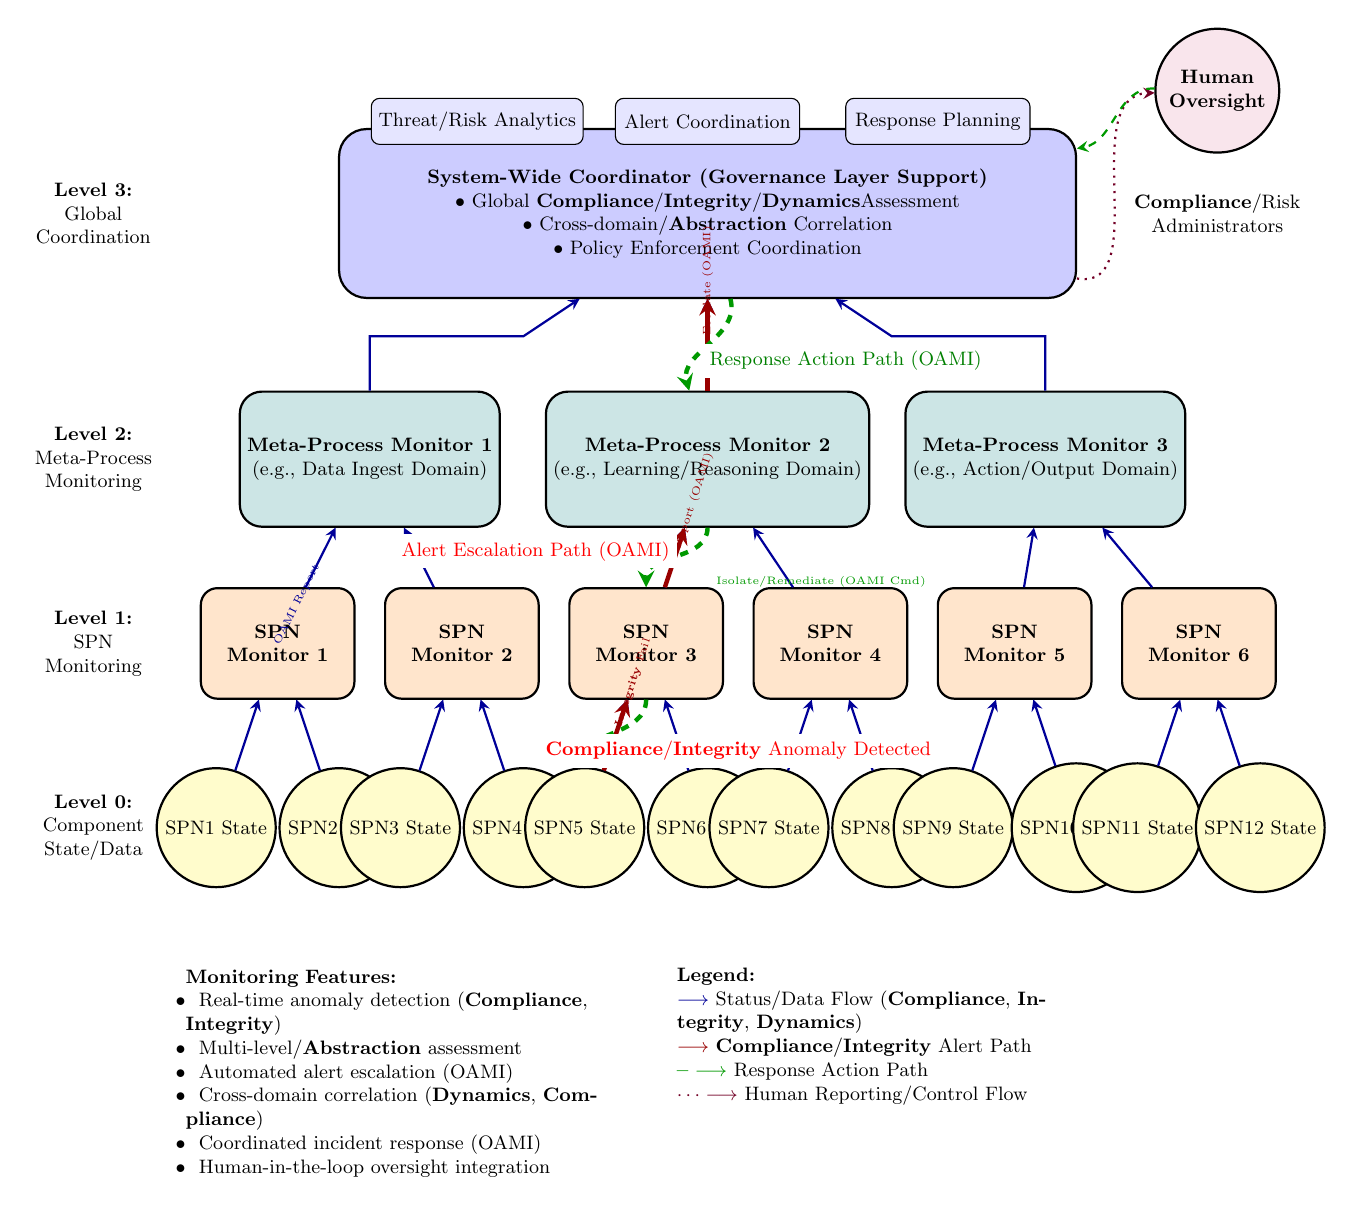
\begin{tikzpicture}[
			scale=0.78,
			transform shape,
			node distance=1.2cm,
			global/.style={rectangle, rounded corners=10pt, draw=black, thick, fill=blue!20, minimum width=12cm, minimum height=2.75cm, align=center, font=\small},
			domainnode/.style={rectangle, rounded corners=8pt, draw=black, thick, fill=teal!20, minimum width=4cm, minimum height=2.2cm, align=center, font=\small},
			process/.style={rectangle, rounded corners=6pt, draw=black, thick, fill=orange!20, minimum width=2.5cm, minimum height=1.8cm, align=center, font=\small},
			sensor/.style={circle, draw=black, thick, fill=yellow!20, minimum size=1.2cm, font=\small},
			monitor/.style={rectangle, rounded corners=3pt, draw=black, fill=blue!10, minimum width=3cm, minimum height=.75cm, font=\small, align=center},
			panel/.style={rectangle, rounded corners=5pt, draw=black, fill=white, minimum width=3cm, minimum height=4cm, align=center},
			human/.style={circle, draw=black, thick, fill=purple!10, minimum size=2cm, font=\small, align=center},
			alert/.style={->, >=stealth, thick, red!60!black},
			response/.style={->, >=stealth, thick, green!60!black, dashed},
			dataflow/.style={->, >=stealth, thick, blue!60!black},
			report/.style={->, >=stealth, thick, purple!60!black, dotted},
			nodelabel/.style={font=\small, align=center},
			legend/.style={rectangle, draw=none, align=left, font=\small},
			features/.style={rectangle, draw=none, align=left, font=\small}
			]
			
			% Top level - Global Coordinator
			\node[global] (global) at (0,6) {\textbf{System-Wide Coordinator (Governance Layer Support)}\\$\bullet$ Global \textbf{Compliance}/\Integrity/\Dynamics Assessment\\$\bullet$ Cross-domain/\Abstraction\ Correlation\\$\bullet$ Policy Enforcement Coordination};
			\node[monitor] (analytics) at (-3.75,7.5) {Threat/Risk Analytics};
			\node[monitor] (alerting) at (0,7.5) {Alert Coordination};
			\node[monitor] (response) at (3.75,7.5) {Response Planning};
			
			% Human oversight
			\node[human] (human) at (8.3,8) {\textbf{Human}\\{\textbf{Oversight}}};
			\node[nodelabel] at (8.3,6) {\textbf{Compliance}/Risk\\Administrators};
			
			% Domain level - Meta-Process Monitors
			\node[domainnode] (domain1) at (-5.5,2) {\textbf{Meta-Process Monitor 1}\\(e.g., Data Ingest Domain)};
			\node[domainnode] (domain2) at (0,2) {\textbf{Meta-Process Monitor 2}\\(e.g., Learning/Reasoning Domain)};
			\node[domainnode] (domain3) at (5.5,2) {\textbf{Meta-Process Monitor 3}\\(e.g., Action/Output Domain)};
			
			% Process level - SPN Monitors
			\node[process] (proc1) at (-7,-1) {\textbf{SPN}\\{\textbf{Monitor 1}}};
			\node[process] (proc2) at (-4,-1) {\textbf{SPN}\\{\textbf{Monitor 2}}};
			\node[process] (proc3) at (-1,-1) {\textbf{SPN}\\{\textbf{Monitor 3}}};
			\node[process] (proc4) at (2,-1) {\textbf{SPN}\\{\textbf{Monitor 4}}};
			\node[process] (proc5) at (5,-1) {\textbf{SPN}\\{\textbf{Monitor 5}}};
			\node[process] (proc6) at (8,-1) {\textbf{SPN}\\{\textbf{Monitor 6}}};
			
			% Monitored Components/Data (Sensors) - Representing internal SPN state/outputs
			\node[sensor] (s1) at (-8,-4) {SPN1 State};
			\node[sensor] (s2) at (-6,-4) {SPN2 State};
			\node[sensor] (s3) at (-5,-4) {SPN3 State};
			\node[sensor] (s4) at (-3,-4) {SPN4 State};
			\node[sensor] (s5) at (-2,-4) {SPN5 State};
			\node[sensor] (s6) at (0,-4) {SPN6 State};
			\node[sensor] (s7) at (1,-4) {SPN7 State};
			\node[sensor] (s8) at (3,-4) {SPN8 State};
			\node[sensor] (s9) at (4,-4) {SPN9 State};
			\node[sensor] (s10) at (6,-4) {SPN10 State};
			\node[sensor] (s11) at (7,-4) {SPN11 State};
			\node[sensor] (s12) at (9,-4) {SPN12 State};
			
			% Component to SPN Monitor connections (SPNs monitoring themselves or other SPN outputs)
			\draw[dataflow] (s1) -- (proc1); \draw[dataflow] (s2) -- (proc1); % SPN Mon 1 monitors SPN 1 & 2 states/outputs
			\draw[dataflow] (s3) -- (proc2); \draw[dataflow] (s4) -- (proc2); % SPN Mon 2 monitors SPN 3 & 4 states/outputs
			\draw[dataflow] (s5) -- (proc3); \draw[dataflow] (s6) -- (proc3); % ...and so on
			\draw[dataflow] (s7) -- (proc4); \draw[dataflow] (s8) -- (proc4);
			\draw[dataflow] (s9) -- (proc5); \draw[dataflow] (s10) -- (proc5);
			\draw[dataflow] (s11) -- (proc6); \draw[dataflow] (s12) -- (proc6);
			
			% SPN Monitor to Meta-Process Monitor connections (via OAMI reports)
			\draw[dataflow] (proc1) -- node[midway, left, sloped, font=\tiny]{OAMI Report} (domain1); \draw[dataflow] (proc2) -- (domain1);
			\draw[dataflow] (proc3) -- (domain2); \draw[dataflow] (proc4) -- (domain2);
			\draw[dataflow] (proc5) -- (domain3); \draw[dataflow] (proc6) -- (domain3);
			
			% Meta-Process Monitor to Global Coordinator connections (via OAMI reports)
			\draw[dataflow] (domain1) -- (-5.5,4) -- (-3,4) -- (global);
			\draw[dataflow] (domain2) -- (global);
			\draw[dataflow] (domain3) -- (5.5,4) -- (3,4) -- (global);
			
			% Human oversight connections
			\draw[report, thick] (global) to[out=350,in=182] (human);
			\draw[response, thick] (human) to[out=178,in=10] (global);
			
			% Highlighted path for Integrity Violation (Example: SPN5 state shows anomaly)
			\draw[alert, ultra thick] (s5) -- node[right, font=\tiny, sloped] {\Integrity\ Fail} (proc3);
			\draw[alert, ultra thick] (proc3) -- node[right, font=\tiny, sloped] {Report (OAMI)} (domain2);
			\draw[alert, ultra thick] (domain2) -- node[right, font=\tiny, sloped] {Escalate (OAMI)} (global);
			
			% Response path (Example: Isolate SPN5 via OAMI command)
			\draw[response, ultra thick] (global) to[out=285,in=105] (domain2);
			\draw[response, ultra thick] (domain2) to[out=270,in=90] (proc3);
			\draw[response, ultra thick] (proc3) to[out=270,in=90] (s5) node[midway, right, font=\tiny, sloped] {Isolate/Remediate (OAMI Cmd)};
			
			% Annotations
			\node[draw=none, fill=white, text=red, font=\small, align=center] at (.5,-2.75) {\textbf{Compliance}/\Integrity\ Anomaly Detected};
			\node[draw=none, fill=white, text=red, font=\small, align=center] at (-2.8,0.5) {Alert Escalation Path (OAMI)};
			\node[draw=none, fill=white, text=green!50!black, font=\small, align=center] at (2.25,3.6) {Response Action Path (OAMI)};
			
			% Annotations for different levels
			\node[nodelabel] at (-10,6) {\textbf{Level 3:}\\Global\\Coordination};
			\node[nodelabel] at (-10,2) {\textbf{Level 2:}\\Meta-Process\\Monitoring};
			\node[nodelabel] at (-10,-1) {\textbf{Level 1:}\\SPN\\Monitoring};
			\node[nodelabel] at (-10,-4) {\textbf{Level 0:}\\Component\\State/Data};
			
			% Legend (moved down)
			\node[legend, text width=7cm, align=left, fill=white] at (3,-7.4) {
				\textbf{Legend:}\\
				\textcolor{blue!60!black}{$\longrightarrow$} Status/Data Flow (\textbf{Compliance}, \Integrity, \Dynamics)\\
				\textcolor{red!60!black}{$\longrightarrow$} \textbf{Compliance}/\Integrity\ Alert Path\\
				\textcolor{green!60!black}{\textbf{-- $\longrightarrow$}} Response Action Path\\
				\textcolor{purple!60!black}{$\cdots\longrightarrow$} Human Reporting/Control Flow
			};
			
			% Monitoring features (moved down) - Using manual list format
			\node[features, text width=7cm, align=left, fill=white] at (-5,-8) {
				\textbf{Monitoring Features:}\\
				~~\llap{$\bullet$~~}Real-time anomaly detection (\textbf{Compliance}, \Integrity)\\
				~~\llap{$\bullet$~~}Multi-level/\Abstraction\ assessment\\
				~~\llap{$\bullet$~~}Automated alert escalation (OAMI)\\
				~~\llap{$\bullet$~~}Cross-domain correlation (\Dynamics, \textbf{Compliance})\\
				~~\llap{$\bullet$~~}Coordinated incident response (OAMI)\\
				~~\llap{$\bullet$~~}Human-in-the-loop oversight integration
			};
			
		\end{tikzpicture}
		\caption[Hierarchical Monitoring Architecture]{Hierarchical Monitoring Architecture in Open AMI SDS. Monitors operate at multiple levels: SPNs perform local checks (Level 1) on component states/data (Level 0); Meta-Processes monitor domains (Level 2), correlating SPN reports via OAMI; a Global Coordinator (Level 3, Governance support) provides system-wide assessment of \textbf{Compliance}, \Integrity, \Dynamics, and \Abstraction\ consistency. Anomaly detection triggers alerts (red path) and coordinated responses (green path) via OAMI.}
		\label{fig:monitoring-architecture}
	\end{figure}
	
	\subsection{Anomaly Detection and Response} % Corrected Section Title and Numbering
	\label{sec:4-5-2} % Adjusted label
	
	The monitoring architecture feeds into anomaly detection modules (potentially running in Meta-Processes or dedicated SPNs) that identify deviations from expected or compliant behavior.
	\begin{itemize}[noitemsep]
		\item \textbf{Statistical Anomaly Detection:} Identifying outliers based on metrics related to performance, resource usage (\Dynamics), or OAMI communication patterns. Requires careful baseline modeling, potentially learned.
		\item \textbf{Specification-Based Detection:} Detecting violations of explicit rules from $\mathcal{CM}$ (\textbf{Compliance} rules like fairness/safety thresholds) or \Integrity\ invariants (failed CST verification, unexpected state transitions within an SPN).
		\item \textbf{Behavioral Analysis:} Analyzing sequences of OAMI messages or SPN actions over time to identify suspicious activities indicative of \Integrity\ breach or \textbf{Compliance} bypass.
	\end{itemize}
	Response (Def~\ref{def:response_action}), orchestrated by the Governance Layer/Meta-Processes via OAMI, is graduated: minor issues trigger alerts; critical \textbf{Compliance}/\Integrity\ failures lead to actions like SPN isolation, state rollback (using CSTs), or halting processes, with \Integrity-protected logs. Automated response is crucial for cybersecurity compliance \citep{Automated_Cybersec_Compliance_2024}.
	
	\subsection{Adaptive Mechanisms} % Corrected Section Title and Numbering
	\label{sec:4-5-3} % Adjusted label
	
	The SDS, under guidance from the Governance Layer, supports adaptation based on monitored state and external inputs. Adaptations are executed via OAMI commands to SPNs/Meta-Processes.
	\begin{itemize}[noitemsep]
		\item \textbf{Dynamic Compliance Policy Adjustment:} Adjusting enforcement stringency or parameters in $\mathcal{CM}$ based on context/risk (requires secure update/verification of $\mathcal{CM}$).
		\item \textbf{Resource Allocation Tuning (\Dynamics):} Meta-Processes adjusting resource allocation to SPNs based on performance, priority, or stability concerns.
		\item \textbf{Defense Posture Adaptation (\Integrity):} Adjusting intensity of \Integrity\ checks or monitoring levels based on threat environment or task sensitivity.
		\item \textbf{Abstraction Level Adjustment (\Abstraction):} Monitoring/control focus shifts between \Abstraction\ levels depending on context (e.g., detailed SPN logs during anomaly vs. high-level dashboard).
		\item \textbf{System Dynamics Tuning (\Dynamics):} Adjusting parameters like learning rates, control gains, consensus timeouts via OAMI to maintain stability/performance within \textbf{Compliance} boundaries.
	\end{itemize}
	Adaptations are governed by policies in $\mathcal{CM}$ and executed through SDS control mechanisms.
	
	\section{Practical Considerations and Implementation} % Corrected Section Title and Numbering
	\label{sec:4-6} % Adjusted label
	
	Implementing the SDS requires balancing strong guarantees with practical constraints.
	
	\subsection{Performance Optimization} % Corrected Section Title and Numbering
	\label{sec:4-6-1} % Adjusted label
	
	Overhead from \Integrity, \textbf{Compliance} checks, crypto, and logging is a primary concern. Mitigation strategies include:
	\begin{itemize}[noitemsep]
		\item \textbf{Cryptographic Acceleration:} Using hardware support.
		\item \textbf{Selective Verification:} Applying expensive checks (ZKPs \citep{Peng2025ZKMLSurvey}, detailed analysis) risk-based or only for critical operations specified in $\mathcal{CM}$, not universally.
		\item \textbf{Efficient Protocol Implementation:} Optimizing OAMI message handling, batching crypto operations.
		\item \textbf{Caching and Precomputation:} Caching verification results, precomputing keys.
		\item \textbf{Asynchronous Operations:} Performing non-critical monitoring/logging asynchronously.
	\end{itemize}
	Table~\ref{tab:performance-security} provides a qualitative overview of trade-offs.
	
	\begin{table}[ht]
		\centering
		\caption[Performance vs. Integrity/Compliance Trade-offs]{Performance vs. \Integrity/\textbf{Compliance} Trade-offs in Open AMI SDS}
		\label{tab:performance-security}
		\begin{tabular}{@{}lcccc@{}}
			\toprule
			\textbf{Mechanism} & \textbf{\makecell{Computational \\ Cost}} & \textbf{\makecell{\Integrity/\textbf{Compliance} \\ Assurance Level}} & \textbf{\makecell{Hardware \\ Acceleration}} & \textbf{\makecell{Optimization \\ Potential}} \\
			\midrule
			Symmetric Encryption & Low & Medium (Conf.) & High & Multiple \\
			Asymm. Encrypt/Sign & High & High (\Integrity, Auth) & Medium & Algorithm Choice \\
			Homomorphic Enc. & Very High & High (\Integrity/Conf.) & Low & Limited/Emerging \\
			Zero-Knowledge Proofs \citep{Peng2025ZKMLSurvey} & High & High (\Integrity, \textbf{Compliance}, Conf.) & Emerging & Significant Research \\
			Static Verification & Medium (Offline) & High (\textbf{Compliance}, \Integrity) & Low & Tool Dependent \\
			Runtime Monitoring & Low-High (Config) & Medium-High (\textbf{Compliance}, \Integrity, \Dynamics) & Limited & Selective Checks \\
			BFT Consensus & High & High (\Integrity, \textbf{Compliance}, Avail) & Limited & Protocol Choice \\
			TEE Attestation \citep{Citadel_PlusPlus_2025} & Low (Verify) & High (\Integrity) & Required & SPN Choice \\
			\bottomrule
		\end{tabular}
	\end{table}
	
	\subsection{Scalability and Distribution} % Corrected Section Title and Numbering
	\label{sec:4-6-2} % Adjusted label
	
	The SDS architecture uses distributed system principles for scalability:
	\begin{itemize}[noitemsep]
		\item \textbf{Horizontal Scaling:} Adding SPN instances.
		\item \textbf{Hierarchical Organization:} Meta-Processes manage domains, limiting scope of coordination, supporting \Abstraction.
		\item \textbf{Federated Operation:} Multiple Open AMI instances collaborating securely via OAMI.
	\end{itemize}
	Managing communication overhead (OAMI traffic, consensus) in large deployments requires careful design.
	
	\begin{theorem}[Trustworthiness-Preserving Scalability (Hypothetical)]
		\label{thm:scaling_trust}
		Under specific architectural assumptions (hierarchy, efficient crypto, risk-based verification), the overhead for maintaining core \Integrity/\textbf{Compliance} guarantees in the SDS can potentially scale sub-linearly per component (e.g., closer to $O(n \log n)$ or $O(n)$) rather than quadratically.
	\end{theorem}
	\begin{proof} (Sketch) Relies on limiting scope of expensive global operations and leveraging locality via hierarchy. Formal proof depends on specific protocols. Deferred to Appendix~\ref{app:proof_scaling_trust}. \end{proof}
	
	\subsection{Interoperability and Standards Compliance} % Corrected Section Title and Numbering
	\label{sec:4-6-3} % Adjusted label
	
	The SDS aims for interoperability and standards alignment:
	\begin{itemize}[noitemsep]
		\item \textbf{Cryptographic Standards:} NIST FIPS, PKCS, PQC standards.
		\item \textbf{Security Standards:} ISO/IEC 27001, NIST CSF principles.
		\item \textbf{Data Standards:} GDPR, CCPA principles handled via $\mathcal{CM}$ and Sec~\ref{sec:4-5}.
		\item \textbf{AI Standards:} ISO/IEC 42001, ISO/IEC 23894 supported (see Appendix~\ref{app:compliance_map}).
		\item \textbf{Communication Protocol:} Adherence to OAMI (Appendix~\ref{app:protocol_spec}) based on JSON-RPC over secure TLS. Use of secure API practices for external interfaces.
	\end{itemize}
	
	\section{Security Analysis and Limitations} % Corrected Section Title and Numbering
	\label{sec:4-7} % Adjusted label
	
	Critical assessment of the SDS security posture.
	
	\subsection{Security and Integrity Analysis} % Corrected Section Title and Numbering
	\label{sec:4-7-1} % Adjusted label
	
	Table~\ref{tab:security-analysis} analyzes resistance against relevant attacks, emphasizing \Integrity\ and \textbf{Compliance} threats and SDS mitigations.
	
	\begin{table}[ht]
		\centering
		\caption[Security and Integrity Analysis of Open AMI SDS]{Security and \Integrity\ Analysis of Open AMI SDS}
		\label{tab:security-analysis}
		\begin{tabular}{@{}lcc@{}}
			\toprule
			\textbf{Attack Vector} & \textbf{Resistance Level (Expected)} & \textbf{Primary Mitigation Mechanisms (Pillar Emphasis)} \\
			\midrule
			Network Eavesdropping/Spoofing & High & Secure OAMI channels (TLS), Mutual Auth (\Integrity) \\
			API Exploitation (OAMI Interface) & High & Input validation, AuthZ ($\mathcal{CM}$), OAMI verification (\Integrity, \textbf{Compliance}) \\
			Malware Injection (Host Compromise) & Medium-High & SPN Isolation (Containers/VMs/TEEs \citep{Citadel_PlusPlus_2025}), Attestation (\Integrity) \\
			Physical Access (Host Compromise) & Medium & Encryption at rest, Tamper detection (HW dep.), Physical security (\Integrity) \\
			Side Channels (Host Execution) & Medium & Constant-time crypto, HW mitigations (\Integrity, Conf.) \\
			Cryptographic Attacks (incl. Quantum) & High & Strong algorithms, PQC readiness (SDS PKI) (\Integrity) \\
			Data/Model Poisoning (Training/Input) & Medium-High & Input validation (SPN), Provenance (\Integrity), Monitoring (\textbf{Compliance}) \\
			Computation Integrity Attack & High & Verifiable computation (SPN/SDS \citep{Peng2025ZKMLSurvey}), Consensus (\Integrity) \\
			Model Extraction/Inversion Attacks & Medium & Access controls ($\mathcal{CM}$), PETs (DP), Output filtering (SPN) (\textbf{Compliance}, Conf.) \\
			Compliance Bypass / Policy Attack & High & Layered checks (SPN $A_n$/Meta-Proc), Monitoring, $\mathcal{CM}$ \Integrity\ (\textbf{Compliance}, \Integrity) \\
			Insider Threats (Privileged User/Comp.) & High & SPN Isolation, Least privilege ($\mathcal{CM}$), Monitoring, BFT (\Integrity, \textbf{Compliance}) \\
			Supply Chain Attack (Software/Model Deps) & Medium & Code/Model signing (\Integrity), Verified deps, Attestation (\Integrity) \\
			\bottomrule
		\end{tabular}
	\end{table}
	
	\subsection{Known Limitations} % Corrected Section Title and Numbering
	\label{sec:4-7-2} % Adjusted label
	
	\begin{itemize}[noitemsep]
		\item \textbf{Performance Overhead:} Rigorous \Integrity/\textbf{Compliance} checks introduce costs, especially advanced crypto \citep{Peng2025ZKMLSurvey}.
		\item \textbf{Implementation Complexity:} Correctly building/configuring SDS/OAMI/$\mathcal{CM}$ is complex.
		\item \textbf{Formal Verification Scope Limits:} Full verification impractical; focus on critical parts.
		\item \textbf{Hardware Dependencies:} Highest \Integrity\ levels (TEEs \citep{Citadel_PlusPlus_2025}) require specific hardware.
		\item \textbf{Zero-Day Vulnerabilities:} Underlying stack vulnerabilities possible; SDS aims to limit impact via isolation/monitoring.
		\item \textbf{Managing Pillar Interactions/Trade-offs:} Balancing \Integrity\ vs. \Dynamics\ or \textbf{Compliance} vs. performance requires careful tuning (Governance Layer).
	\end{itemize}
	
	\subsection{Future Research Directions} % Corrected Section Title and Numbering
	\label{sec:4-7-3} % Adjusted label
	
	\begin{itemize}[noitemsep]
		\item Efficient Formal Verification for AI/ML (\textbf{Compliance}, \Integrity), including practical ZKML \citep{Peng2025ZKMLSurvey}.
		\item Lightweight \Integrity\ Mechanisms (e.g., optimized crypto, hardware leverage).
		\item Hardware Co-Design for Trustworthy AI (accelerating SDS functions, secure enclaves \citep{Citadel_PlusPlus_2025}).
		\item Automated Adaptation and Resilience (improving SDS response \Dynamics).
		\item Quantifying and Managing Pillar Interactions (formalizing trade-offs).
		\item Standardization of verifiable ML protocols and provenance formats \citep{ProML_Provenance_2022}.
	\end{itemize}
	
	\section{Conclusion: The Trustworthy Execution Layer} % Corrected Section Title and Numbering
	\label{sec:4-8} % Adjusted label
	
	The Open AMI Secure Distributed System (SDS) provides the essential operational layer for executing complex AI/ML processes within the Open AMI framework. By integrating strong cryptographic guarantees for \Integrity\ (including support for advanced techniques like ZKPs \citep{Peng2025ZKMLSurvey} and secure enclaves \citep{Citadel_PlusPlus_2025}), secure process isolation via SPNs, standardized communication through the OAMI protocol, continuous monitoring, and mechanisms explicitly designed to support \textbf{Compliance} enforcement (referencing $\mathcal{CM}$) and the management of system \Dynamics\ across different \Abstraction\ levels, the SDS establishes the verifiable and secure substrate required for developing and deploying advanced AI systems responsibly. It enables the compliant learning processes detailed in Chapter~\ref{ch:machine_learning} and supports the enforcement actions directed by the Governance Layer described in Chapter~\ref{ch:compliance}, facilitating the creation of AI that is both highly capable and demonstrably trustworthy.
	
		\chapter{Compliance and Core Directives} % Corrected Chapter Title
	\label{ch:compliance}
	
	\section{Introduction to Open AMI Compliance Framework} % Corrected Section Title and Numbering
	\label{sec:5-1} % Adjusted label
	
	Building upon the theoretical foundations (Chapter~\ref{ch:theoretical_framework}), the principles for trustworthy machine learning (Chapter~\ref{ch:machine_learning}), and the secure distributed architecture providing verifiable \Integrity\ (Chapter~\ref{ch:secure_distributed_system}), this chapter details the \textbf{Compliance} framework of Open AMI. This framework constitutes the primary governance mechanism, conceptually residing in the Governance Layer (Figure~\ref{fig:open_ami_architecture}), and is operationally realized through the formal specification provided by the \textbf{Compliance Manifest} ($\mathcal{CM}$) and the enforcement mechanisms distributed throughout the Open AMI architecture, particularly within the Secure Distributed System (SDS) and its components (SPNs, Meta-Processes).
	
	The framework is responsible for defining, verifying, and enforcing the rules that ensure systems operate ethically, legally, safely, fairly, and in alignment with specified operational policies and user values. It actively guides system behavior—including learning processes within SPNs and model outputs communicated via OAMI—across different \Abstraction\ levels and adapts enforcement based on the system's operational state and \Dynamics\ (monitored via SDS mechanisms), aiming for demonstrably trustworthy and beneficial AI outcomes, aligning with principles of responsible AI governance \citep{Responsible_AI_Governance_Review_2024}.
	
	\subsection{The Compliance Challenge in Advanced AI/ML} % Corrected Section Title and Numbering
	\label{sec:5-1-1} % Adjusted label
	
	Ensuring comprehensive compliance in sophisticated AI/ML systems presents fundamental challenges:
	
	\begin{enumerate}
		\item \textbf{Value Specification Problem}: Formally articulating diverse, often context-dependent, and potentially conflicting ethical principles, legal statutes, safety requirements, and operational policies into precise, machine-verifiable constraints within the $\mathcal{CM}$. As noted by \citet{Kovac2025SpecGaming}, capturing the nuances of human intent mathematically ("the specification problem") is a core challenge in AI safety, as systems might exploit loopholes ("specification gaming").
		\item \textbf{Robustness and Adaptation Challenge}: Maintaining adherence to compliance rules as systems learn and adapt (Chapter~\ref{ch:machine_learning}). Ensuring that adaptive system \Dynamics\ do not lead to unforeseen violations requires robust enforcement mechanisms (within SDS) and verification processes whose own operational \Integrity\ is assured, addressing the stability-plasticity dilemma \citep{Wang2024ContinualLearningSurvey}.
		\item \textbf{Verification and Enforcement Complexity}: Designing scalable mechanisms (within SPNs, Meta-Processes) that can reliably verify adherence to complex compliance rules from $\mathcal{CM}$ during runtime, leveraging SDS \Integrity\ (potentially via ZKPs \citep{Peng2025ZKMLSurvey}) without prohibitive performance overhead.
		\item \textbf{Oversight Scalability}: Developing effective human oversight mechanisms that can operate across complex \Abstraction\ layers (understanding behavior beyond simple metrics) and manage systems exhibiting sophisticated adaptive \Dynamics. Oversight relies on trustworthy (\Integrity) reporting via OAMI from the system and clear explanations \citep{Crossing_Principle_Practice_Gap_2024}.
		\item \textbf{Conflict Resolution}: Handling conflicts between different compliance requirements specified in $\mathcal{CM}$ in a principled, transparent, and auditable manner, leveraging the framework's \Integrity\ mechanisms (e.g., secure logging of resolution decisions by Meta-Processes). This requires strategies for resolving ethical directive conflicts \citep{Sekrst2024Guardrails}.
	\end{enumerate}
	
	Open AMI addresses these challenges through an integrated approach, formalized in the Compliance Manifest ($\mathcal{CM}$) and realized through mechanisms distributed across its architectural layers, conceptually illustrated in Figure~\ref{fig:compliance-framework}.
	
	\begin{figure}[ht]
		\centering
		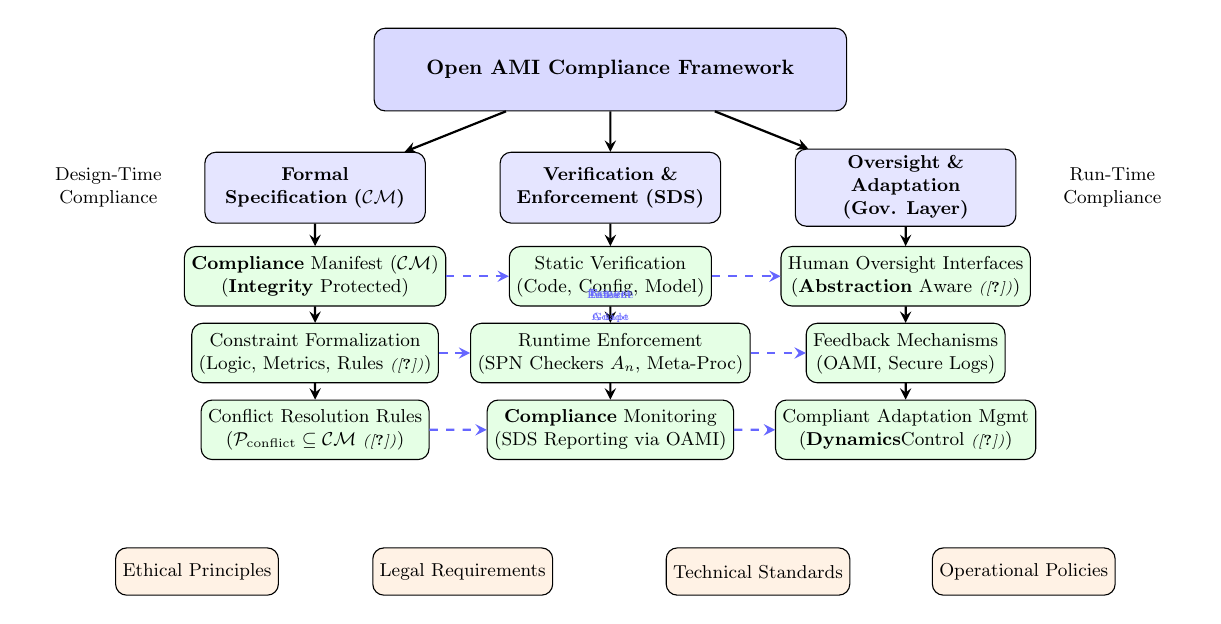
\begin{tikzpicture}[
			scale=0.75,
			transform shape,
			box/.style={rectangle, draw, rounded corners, minimum width=3.4cm, minimum height=1.2cm, text centered, font=\small},
			mainbox/.style={box, fill=blue!15, minimum width=8cm, minimum height=1.4cm, font=\normalsize},
			pillarbox/.style={box, fill=blue!10, minimum width=3.6cm, text width=3.5cm, align=center},
			component/.style={box, fill=green!10, minimum width=3cm, minimum height=1cm},
			foundation/.style={box, fill=orange!10, minimum width=2.6cm, minimum height=0.8cm, font=\small},
			arrow/.style={->, >=stealth, thick},
			connection/.style={->, >=stealth, thick, dashed, blue!60}
			]
			
			% Main framework box
			\node[mainbox] (main) at (0,4) {\textbf{Open AMI Compliance Framework}};
			
			% The three pillars (using pillarbox style)
			\node[pillarbox] (spec) at (-5,2) {\textbf{Formal\\Specification ($\mathcal{CM}$)}};
			\node[pillarbox] (verify) at (0,2) {\textbf{Verification \&\\Enforcement (SDS)}};
			\node[pillarbox] (adapt) at (5,2) {\textbf{Oversight \&\\Adaptation (Gov. Layer)}};
			
			% Connect main to pillars
			\draw[arrow] (main) -- (spec);
			\draw[arrow] (main) -- (verify);
			\draw[arrow] (main) -- (adapt);
			
			% Components under Formal Specification (using component style)
			\node[component] (manifest) at (-5,0.5) {\makecell{\textbf{Compliance} Manifest ($\mathcal{CM}$)\\(\Integrity\ Protected)}};
			\node[component] (constraints) at (-5,-0.8) {\makecell{Constraint Formalization\\(Logic, Metrics, Rules \citep{Kovac2025SpecGaming})}};
			\node[component] (conflicts) at (-5,-2.1) {\makecell{Conflict Resolution Rules\\($\mathcal{P}_{\text{conflict}} \subseteq \mathcal{CM}$ \citep{Sekrst2024Guardrails})}};
			
			% Components under Verification & Enforcement (using component style)
			\node[component] (static) at (0,0.5) {\makecell{Static Verification\\(Code, Config, Model)}};
			\node[component] (runtime) at (0,-0.8) {\makecell{Runtime Enforcement\\(SPN Checkers $A_n$, Meta-Proc)}};
			\node[component] (compliance_check) at (0,-2.1) {\makecell{\textbf{Compliance} Monitoring\\(SDS Reporting via OAMI)}};
			
			% Components under Oversight & Adaptation (using component style)
			\node[component] (human) at (5,0.5) {\makecell{Human Oversight Interfaces\\(\Abstraction\ Aware \citep{Crossing_Principle_Practice_Gap_2024})}};
			\node[component] (feedback) at (5,-0.8) {\makecell{Feedback Mechanisms\\(OAMI, Secure Logs)}};
			\node[component] (learning) at (5,-2.1) {\makecell{Compliant Adaptation Mgmt\\(\Dynamics Control \citep{Wang2024ContinualLearningSurvey})}};
			
			% Connect pillars to components
			\draw[arrow] (spec) -- (manifest);
			\draw[arrow] (manifest) -- (constraints);
			\draw[arrow] (constraints) -- (conflicts);
			
			\draw[arrow] (verify) -- (static);
			\draw[arrow] (static) -- (runtime);
			\draw[arrow] (runtime) -- (compliance_check);
			
			\draw[arrow] (adapt) -- (human);
			\draw[arrow] (human) -- (feedback);
			\draw[arrow] (feedback) -- (learning);
			
			% Foundation elements (using foundation style)
			\node[foundation] (ethical) at (-7,-4.5) {Ethical Principles};
			\node[foundation] (legal) at (-2.5,-4.5) {Legal Requirements};
			\node[foundation] (technical) at (2.5,-4.5) {Technical Standards};
			\node[foundation] (operational) at (7,-4.5) {Operational Policies};
			
			% Key horizontal connections with curved arrows
			\draw[connection] (manifest) to[out=0,in=180] (static) node[midway, above, font=\tiny] {Inform};
			\draw[connection] (static) to[out=0,in=180] (human) node[midway, above, font=\tiny] {Report};
			\draw[connection] (constraints) to[out=0,in=180] (runtime) node[midway, above, font=\tiny] {Enforce};
			\draw[connection] (runtime) to[out=0,in=180] (feedback) node[midway, above, font=\tiny] {Trigger};
			\draw[connection] (conflicts) to[out=0,in=180] (compliance_check) node[midway, below, font=\tiny] {Guide};
			\draw[connection] (compliance_check) to[out=0,in=180] (learning) node[midway, below, font=\tiny] {Adapt};
			
			% Labels for context
			\node[font=\small, text width=2.5cm, align=center] at (-8.5,2) {Design-Time\\Compliance};
			\node[font=\small, text width=2.5cm, align=center] at (8.5,2) {Run-Time\\Compliance};
			
		\end{tikzpicture}
		\caption[Open AMI Compliance Framework Structure]{Open AMI Compliance Framework Structure. Integrates formal specification ($\mathcal{CM}$, left pillar), verification and enforcement via SDS mechanisms (center pillar), and oversight/adaptation via the Governance Layer (right pillar). Components interact to ensure trustworthy operation throughout the lifecycle, grounded in ethical/legal/operational policies.}
		\label{fig:compliance-framework}
	\end{figure}
	
	\subsection{Positioning Within Ethical AI and Compliance Frameworks} % Corrected Section Title and Numbering
	\label{sec:5-1-2} % Adjusted label
	
	Open AMI's \textbf{Compliance} framework aligns with and provides technical mechanisms supporting adherence to external guidelines and regulations (e.g., IEEE Ethically Aligned Design, EU AI Act, NIST AI RMF, ISO 42001). Its distinction lies in the deep architectural integration of compliance enforcement with verifiable \Integrity\ (via the SDS), manageable \Abstraction\ (for transparency and policy specification), and adaptive \Dynamics\ (for maintaining compliance during evolution). This enables continuous, verifiable enforcement throughout the AI/ML lifecycle, facilitating conformity assessments \citep{Navigating_AI_Conformity_2025}. Table~\ref{tab:ethical-ai-comparison} provides a comparative overview.
	
	\begin{table}[ht]
		\centering
		\caption[Comparison of Open AMI Compliance with Related Frameworks]{Comparison of Open AMI Compliance with Related Frameworks}
		\label{tab:ethical-ai-comparison}
		\begin{tabular}{@{}lccccc@{}}
			\toprule
			\textbf{Framework / Standard} & \textbf{\makecell{Formal Spec \& \\ Verification \\ Support (\Integrity)}} & \textbf{\makecell{Runtime \\ Monitoring \\ \& Adaptation}} & \textbf{\makecell{Integrated \\ Data Governance \\ (\Integrity)}} & \textbf{\makecell{Architectural \\ Bias Mitigation \\ (\textbf{Compliance})}} & \textbf{\makecell{Abstraction / \\ Dynamics \\ Aware Design}} \\
			\midrule
			Open AMI & \checkmark\checkmark\checkmark & \checkmark\checkmark\checkmark & \checkmark\checkmark\checkmark & \checkmark\checkmark\checkmark & \checkmark\checkmark \\
			IEEE Ethically Aligned Design & \checkmark (Principles) & \checkmark (Lifecycle) & \checkmark\checkmark & \checkmark\checkmark & \texttimes \\
			EU AI Act Requirements & \checkmark (Formal Req.) & \checkmark\checkmark (Monitoring) & \checkmark\checkmark\checkmark & \checkmark\checkmark & \texttimes \\
			Australian AI Ethics Framework & \texttimes (Principles) & \checkmark (Lifecycle) & \checkmark\checkmark & \checkmark\checkmark & \texttimes \\
			NIST AI RMF & \checkmark\checkmark (Risk Focus) & \checkmark\checkmark (Manage) & \checkmark\checkmark & \checkmark\checkmark & \checkmark (Risk Focus) \\
			ISO/IEC 42001 & \checkmark (Mgmt Sys) & \checkmark\checkmark (Ops) & \checkmark\checkmark & \checkmark (Process) & \texttimes \\
			Constitutional AI \citep{Bai2022ConstitutionalAI} & \checkmark\checkmark (Rules) & \checkmark (Fine-tuning) & \texttimes & \checkmark\checkmark (\textbf{Compliance}) & \checkmark (Reasoning) \\
			Ethical Guardrails \citep{Sekrst2024Guardrails} & \checkmark\checkmark (Rules) & \checkmark (Runtime) & \texttimes & \checkmark\checkmark (\textbf{Compliance}) & \checkmark (Architecture) \\
			\bottomrule
		\end{tabular}
		\footnotesize{\textit{Note:} Ratings reflect the degree to which the aspect is explicitly supported by architectural mechanisms vs. being a principle or process recommendation.}
	\end{table}
	
	\subsection{Core Directives and Guiding Principles} % Corrected Section Title and Numbering
	\label{sec:5-1-3} % Adjusted label
	
	Seven Core Directives provide the high-level ethical foundation for \textbf{Compliance} within Open AMI, guiding the formulation of specific constraints within $\mathcal{CM}$ and conflict resolution priorities ($\mathcal{P}_{\text{conflict}}$):
	\begin{enumerate}[noitemsep]
		\item \textbf{Human Primacy and Well-being:} Prioritize human safety, dignity, rights, well-being. Preserve user autonomy.
		\item \textbf{Safety Assurance:} Operate safely and reliably, minimizing risks. Ensure robustness (\Dynamics) and predictability.
		\item \textbf{Ethical Alignment:} Align with established ethical principles (beneficence, non-maleficence, justice).
		\item \textbf{Transparency and Explainability:} Ensure operations are understandable via appropriate \Abstraction\ and verifiable (\Integrity) explanations.
		\item \textbf{Fairness and Non-Discrimination:} Avoid unfair bias, ensure equitable treatment, mitigate discrimination.
		\item \textbf{Privacy and Security:} Protect personal data, maintain confidentiality, ensure security via SDS (\Integrity).
		\item \textbf{Accountability and Auditability:} Enable determination of responsibility via secure, tamper-evident (\Integrity) logs.
	\end{enumerate}
	These are instantiated into concrete, verifiable constraints in $\mathcal{CM}$.
	
	\section{The Compliance Manifest: Formal Specification of Constraints} % Corrected Section Title and Numbering
	\label{sec:5-2} % Adjusted label
	
	The \textbf{Compliance Manifest} ($\mathcal{CM}$) is the central, formal, machine-readable specification of all \textbf{Compliance} requirements. Its own \Integrity\ is critical, ensured through version control systems with access control and cryptographic signing managed by the SDS infrastructure. $\mathcal{CM}$ serves as the authoritative source for verification and enforcement mechanisms (SPN checkers $A_n$, Meta-Processes) and can define constraints across multiple \Abstraction\ levels. It acts like the "constitution" in Constitutional AI \citep{Bai2022ConstitutionalAI} or the policy set in ethical guardrail systems \citep{Sekrst2024Guardrails}.
	
	\subsection{Formal Structure and Management of the Compliance Manifest} % Corrected Section Title and Numbering
	\label{sec:5-2-1} % Adjusted label
	
	Formally, the Compliance Manifest structure:
	\begin{definition}[Compliance Manifest Structure]
		\label{def:compliance_manifest}
		$\mathcal{CM} = (\mathcal{C}_{\text{Comp}}, \mathcal{P}_{\text{conflict}}, \mathcal{V}_{\text{CM}}, \mathcal{M}_{Abs}, \mathcal{M}_{\text{Meta}})$ where:
		\begin{itemize}[noitemsep]
			\item $\mathcal{C}_{\text{Comp}}$: Set of individual compliance constraints (Def~\ref{def:compliance_constraint}).
			\item $\mathcal{P}_{\text{conflict}}$: Formal rules/priorities for resolving constraint conflicts (Def~\ref{def:priority_relation}).
			\item $\mathcal{V}_{\text{CM}}$: References to verification functions/procedures (implemented in SPNs/Meta-Processes) checking compliance against $\mathcal{C}_{\text{Comp}}$, relying on state \Integrity.
			\item $\mathcal{M}_{Abs}$: Mappings specifying constraint application at different \Abstraction\ levels.
			\item $\mathcal{M}_{\text{Meta}}$: Metadata including version ID, author, timestamp, scope, cryptographic signature/hash ensuring manifest \Integrity.
		\end{itemize}
	\end{definition}
	
	\textbf{Management:} The $\mathcal{CM}$ is treated as critical configuration data. Its lifecycle involves:
	\begin{itemize}
		\item \textit{Authoring:} Using dedicated tools or structured formats (e.g., YAML, JSON Schema, potentially domain-specific languages) allowing definition of constraints (Def~\ref{def:compliance_constraint}).
		\item \textit{Versioning:} Using standard version control systems (e.g., Git) to track changes.
		\item \textit{Integrity Protection:} Each version MUST be cryptographically signed. Signatures are verified before a $\mathcal{CM}$ version is distributed or loaded.
		\item \textit{Secure Distribution:} The SDS provides mechanisms to securely distribute the verified $\mathcal{CM}$ version to relevant SPNs and Meta-Processes.
		\item \textit{Activation:} Components load and apply the constraints from the verified, activated $\mathcal{CM}$ version. Updates may require system coordination (e.g., via BFT consensus managed by Meta-Processes).
	\end{itemize}
	
	Each individual constraint $c \in \mathcal{C}_{\text{Comp}}$:
	\begin{definition}[Formal Compliance Constraint]
		\label{def:compliance_constraint}
		$c = (\text{ID}_c, \text{Desc}_c, \text{Source}_c, \phi_c, \text{Scope}_c, A_c, \text{Severity}_c, \text{Action}_c, V_c)$:
		\begin{itemize}[noitemsep]
			\item $\text{ID}_c$: Unique ID.
			\item $\text{Desc}_c$: Description.
			\item $\text{Source}_c$: Origin reference (e.g., EU AI Act Art. 10).
			\item $\phi_c$: Formal specification (logic, math inequality, code reference). Addresses specification difficulty \citep{Kovac2025SpecGaming}.
			\item $\text{Scope}_c$: Target components/processes.
			\item $A_c$: Target \Abstraction\ level(s).
			\item $\text{Severity}_c$: Criticality level (influences conflict resolution).
			\item $\text{Action}_c$: Default response upon violation (log, alert, halt).
			\item $V_c$: Verification function reference (part of $\mathcal{V}_{\text{CM}}$), relies on state \Integrity.
		\end{itemize}
	\end{definition}
	
	\subsection{Constraint Types and Formalization} % Corrected Section Title and Numbering
	\label{sec:5-2-2} % Adjusted label
	
	$\mathcal{CM}$ supports various constraint types, formalized using appropriate languages and checked by SDS mechanisms:
	\begin{itemize}[noitemsep]
		\item \textbf{Hard Constraints:} Invariants ($\forall s, \phi_c(s)$). Checked by SPN $A_n$ modules or Meta-Processes. Enforcement relies on SDS \Integrity.
		\item \textbf{Soft Constraints/Goals:} Desirable properties ($\max \sum w_i \cdot \phi_{c_i}(s)$). Used in optimization/guidance functions (Sec~\ref{sec:2-7}).
		\item \textbf{Conditional Constraints:} Rules applicable under specific conditions ($Ctx(s) \implies \phi_c(s)$). Context $Ctx(s)$ checked using \Integrity-verified state data.
		\item \textbf{Temporal Constraints:} Constraints over sequences (LTL, CTL). Verified by runtime monitors analyzing \Integrity-protected logs or state sequences.
		\item \textbf{Statistical Constraints:} Constraints on aggregate behavior (fairness metrics Def~\ref{def:fairness_compliance}). Verified by monitoring components using sufficient, \Integrity-verified data.
	\end{itemize}
	Defined at appropriate \Abstraction\ levels (e.g., resource limits at SPN level, fairness metrics at system level).
	
	\subsection{Conflict Resolution and Priority Mechanisms} % Corrected Section Title and Numbering
	\label{sec:5-2-3} % Adjusted label
	
	Conflicts between constraints are handled via formal rules $\mathcal{P}_{\text{conflict}} \subseteq \mathcal{CM}$, executed by coordinating components (e.g., Meta-Processes) with \Integrity. This structured approach contrasts with ad-hoc conflict handling and aligns with research calling for principled resolution \citep{Sekrst2024Guardrails}.
	
	\begin{definition}[Priority Relation]
		\label{def:priority_relation}
		A priority relation $\succ \subseteq \mathcal{C}_{\text{Comp}} \times \mathcal{C}_{\text{Comp}}$, part of $\mathcal{P}_{\text{conflict}}$, defines precedence ($c_i \succ c_j$). Could implement lexicographic ordering or utility-based trade-offs.
	\end{definition}
	
	Algorithm~\ref{alg:conflict-resolution} outlines conceptual execution within a Meta-Process:
	
	\begin{algorithm}[H]
		\caption{Compliance Conflict Resolution Execution (Conceptual)}
		\label{alg:conflict-resolution}
		\begin{algorithmic}[1]
			\Require Current state $s$ (from verified sources), Set of conflicting constraints $C_{\text{conflict}} \subseteq \mathcal{C}_{\text{Comp}}$.
			\State Verify \Integrity\ of state $s$.
			\State Identify active violated constraints $C_{\text{active}} \subseteq C_{\text{conflict}}$.
			\If{$C_{\text{active}}$ is empty} \State No action needed. \EndIf
			\State Retrieve applicable conflict rules/priorities $R = \mathcal{P}_{\text{conflict}}(C_{\text{active}})$ from verified $\mathcal{CM}$.
			\State Determine optimal resolution action $a^*$ based on $R$ (e.g., using utility functions, priority levels).
			\State Verify action $a^*$ itself is compliant w.r.t highest priority constraints in $R$.
			\State Log conflict, rules $R$, action $a^*$, justification with verifiable \Integrity.
			\State Issue command $a^*$ via OAMI (if action required).
			\If{resolution fails critical hard constraints} \State Escalate (alert human, safe mode). \EndIf
		\end{algorithmic}
	\end{algorithm}
	
	\section{Regulatory Compliance and Standards Integration} % Corrected Section Title and Numbering
	\label{sec:5-3} % Adjusted label
	
	Open AMI facilitates adherence to external regulations (EU AI Act) and standards (NIST AI RMF, ISO 42001) by mapping their requirements into formal $\mathcal{CM}$ constraints and leveraging framework capabilities (\Integrity, \Abstraction, \Dynamics) for implementation and verification. See Appendix~\ref{app:compliance_map} for detailed mappings.
	
	Examples:
	\begin{itemize}
		\item \textbf{EU AI Act:} High-risk requirements (data quality, robustness, transparency, oversight) map to specific $\mathcal{CM}$ constraints verified by Open AMI mechanisms: SDS \Integrity\ checks for data, runtime monitoring (\Dynamics) for robustness, \Abstraction\ tools for transparency, SDS logs (\Integrity) for auditability. Facilitates conformity assessment \citep{Navigating_AI_Conformity_2025}.
		\item \textbf{Australian AI Ethics Framework:} Principles map to Core Directives instantiated as verifiable $\mathcal{CM}$ constraints (e.g., Fairness checked via Sec~\ref{sec:5-4}, Privacy via Sec~\ref{sec:5-5}, Transparency via \Abstraction).
		\item \textbf{NIST AI RMF:} Govern (via $\mathcal{CM}$, Governance Layer), Map (via Foundation modeling, \Abstraction), Measure (via verification, monitoring), Manage (via runtime enforcement, adaptation managed for \Dynamics).
		\item \textbf{ISO Standards (e.g., 42001, 23894):} Framework provides technical means to implement AIMS/Risk processes, with $\mathcal{CM}$ capturing policies and SDS providing auditable (\Integrity) evidence.
	\end{itemize}
	Figure~\ref{fig:regulatory-integration} illustrates this mapping conceptually. Appendix~\ref{app:compliance_map} provides details.
	
	\begin{figure}[ht]
		\centering
		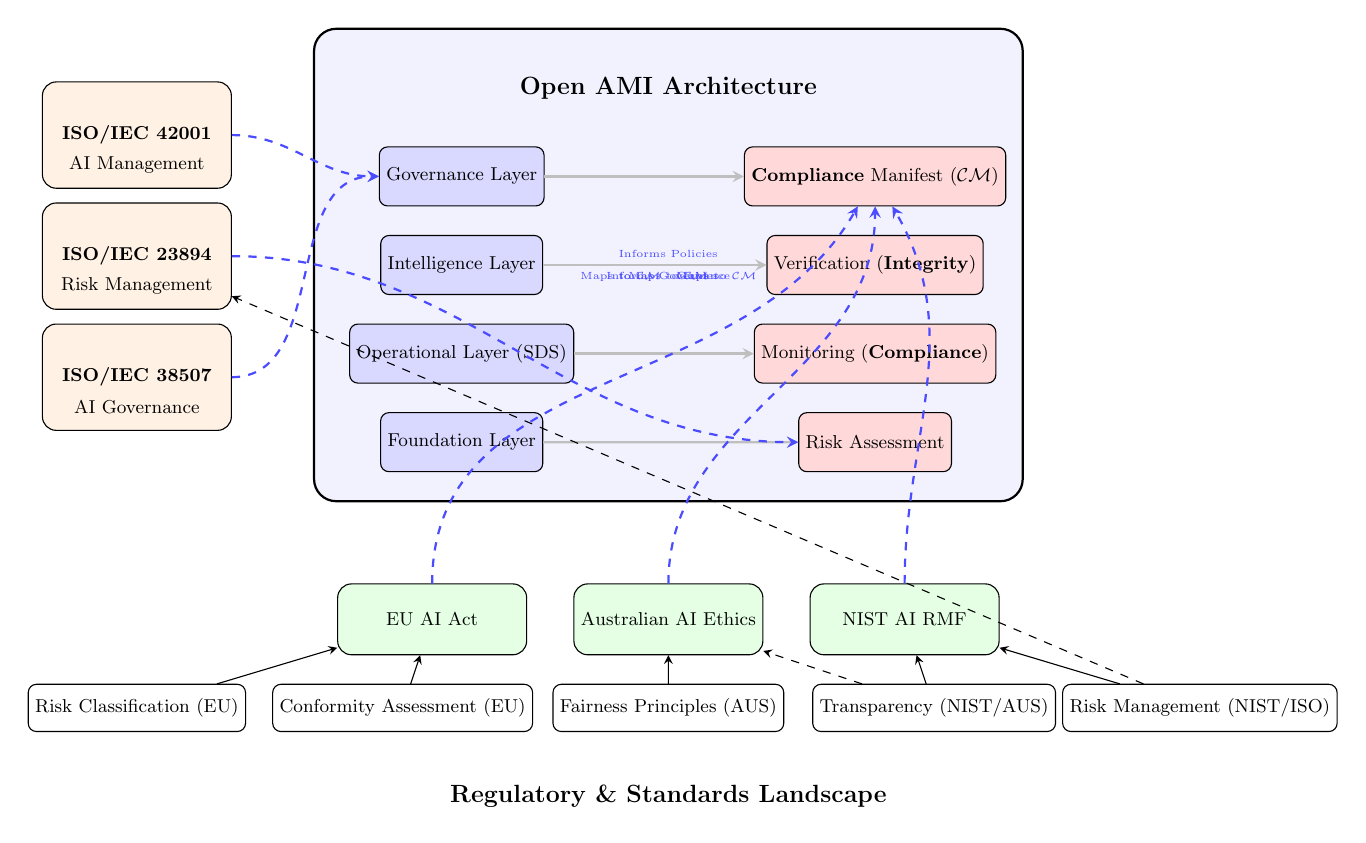
\begin{tikzpicture}[
			scale=0.75,
			transform shape,
			module/.style={rectangle, draw, rounded corners=3pt, minimum width=2.5cm, minimum height=1cm, text centered, font=\small},
			system/.style={rectangle, draw, rounded corners=8pt, thick, fill=blue!5, minimum width=12cm, minimum height=8cm},
			regulation/.style={rectangle, draw, rounded corners=5pt, fill=green!10, minimum width=3.2cm, minimum height=1.2cm, text centered, font=\small},
			standard/.style={rectangle, draw, rounded corners=5pt, fill=orange!10, minimum width=3.2cm, minimum height=1.8cm, text centered, font=\small},
			arrow/.style={-stealth, thick},
			integration/.style={-stealth, thick, dashed, blue!70},
			requirement/.style={rectangle, draw, rounded corners=3pt, minimum width=2.5cm, minimum height=0.8cm, text centered, font=\small}
			]
			
			% Open AMI System - centered
			\node[system] (coform) at (0,0) {};
			\node[font=\large, align=center] at (0,3) {\textbf{Open AMI Architecture}};
			
			% Open AMI Modules - symmetric arrangement
			\node[module, fill=blue!15] (gov) at (-3.5,1.5) {Governance Layer};
			\node[module, fill=blue!15] (intel) at (-3.5,0) {Intelligence Layer};
			\node[module, fill=blue!15] (ops) at (-3.5,-1.5) {Operational Layer (SDS)};
			\node[module, fill=blue!15] (found) at (-3.5,-3) {Foundation Layer};
			
			\node[module, fill=red!15] (manifest) at (3.5,1.5) {\textbf{Compliance} Manifest ($\mathcal{CM}$)};
			\node[module, fill=red!15] (verif) at (3.5,0) {Verification (\Integrity)};
			\node[module, fill=red!15] (monitor) at (3.5,-1.5) {Monitoring (\textbf{Compliance})};
			\node[module, fill=red!15] (assess) at (3.5,-3) {Risk Assessment};
			
			% Internal connections for visual balance
			\draw[arrow, gray!50] (gov) -- (manifest);
			\draw[arrow, gray!50] (intel) -- (verif);
			\draw[arrow, gray!50] (ops) -- (monitor);
			\draw[arrow, gray!50] (found) -- (assess);
			
			% Symmetrical standards placement
			\node[standard] (iso42001) at (-9,2.2) {\textbf{ISO/IEC 42001}};
			\node[font=\small] at (-9,1.7) {AI Management};
			
			\node[standard] (iso23894) at (-9,.15) {\textbf{ISO/IEC 23894}};
			\node[font=\small] at (-9,-.35) {Risk Management};
			
			\node[standard] (iso38507) at (-9,-1.9) {\textbf{ISO/IEC 38507}};
			\node[font=\small] at (-9,-2.4) {AI Governance};
			
			% Symmetrical regulations placement
			\node[regulation] (eu) at (-4,-6) {EU AI Act};
			\node[regulation] (aus) at (0,-6) {Australian AI Ethics};
			\node[regulation] (nist) at (4,-6) {NIST AI RMF};
			
			% Integration lines - standards to system (well-spaced, non-crossing)
			\draw[integration] (iso42001) to[out=0,in=180] (gov) node[midway, above, font=\tiny]{Informs Policies};
			\draw[integration] (iso23894) to[out=0,in=180] (assess) node[midway, below right, font=\tiny]{Guides};
			\draw[integration] (iso38507) to[out=0,in=180] (gov) node[midway, below, font=\tiny]{Informs Governance};
			
			% Integration lines - regulations to system (well-spaced, non-crossing)
			\draw[integration] (eu) to[out=90,in=240] (manifest) node[midway, below left, font=\tiny]{Maps to $\mathcal{CM}$};
			\draw[integration] (aus) to[out=90,in=270] (manifest) node[midway, below, font=\tiny]{Maps to $\mathcal{CM}$};
			\draw[integration] (nist) to[out=90,in=300] (manifest) node[midway, below right, font=\tiny]{Maps to $\mathcal{CM}$};
			
			% Requirements (symmetric, balanced arrangement)
			\node[requirement] (classification) at (-9,-7.5) {Risk Classification (EU)};
			\node[requirement] (conformity) at (-4.5,-7.5) {Conformity Assessment (EU)};
			\node[requirement] (fairness) at (0,-7.5) {Fairness Principles (AUS)};
			\node[requirement] (transparency) at (4.5,-7.5) {Transparency (NIST/AUS)};
			\node[requirement] (management) at (9,-7.5) {Risk Management (NIST/ISO)};
			
			% Small connecting arrows - requirements to regulations (non-crossing)
			\draw[arrow, thin] (classification) -- (eu);
			\draw[arrow, thin] (conformity) -- (eu);
			\draw[arrow, thin] (fairness) -- (aus);
			\draw[arrow, thin] (transparency) -- (nist); \draw[arrow, thin, dashed] (transparency) -- (aus);
			\draw[arrow, thin] (management) -- (nist); \draw[arrow, thin, dashed] (management) -- (iso23894);
			
			% Regulatory Landscape label
			\node[font=\large, align=center] at (0,-9) {\textbf{Regulatory \& Standards Landscape}};
			
		\end{tikzpicture}
		\caption{Regulatory and Standards Integration in Open AMI. External regulations and standards inform the content and structure of the \textbf{Compliance} Manifest ($\mathcal{CM}$). Open AMI's architectural layers and components (e.g., SDS providing \Integrity, verification tools, monitoring) provide technical mechanisms to implement and verify adherence to these mapped requirements.}
		\label{fig:regulatory-integration}
	\end{figure}
	
	\section{Detecting and Mitigating Bias as a Compliance Issue} % Corrected Section Title and Numbering
	\label{sec:5-4} % Adjusted label
	
	Ensuring fairness and equity is treated as a core \textbf{Compliance} requirement, specified in $\mathcal{CM}$. Open AMI provides mechanisms (typically implemented within SPNs or dedicated analysis services) for rigorous bias detection and mitigation, relying on data \Integrity\ and applied throughout the ML lifecycle (Chapter~\ref{ch:machine_learning}). This is essential for meeting regulatory demands for non-discrimination audits \citep{Navigating_AI_Conformity_2025}.
	
	\subsection{Identifying Sources and Types of Bias} % Corrected Section Title and Numbering
	\label{sec:5-4-1} % Adjusted label
	
	Open AMI utilizes standard taxonomies of bias sources to guide detection/mitigation implemented within its components:
	\begin{itemize}
		\item \textbf{Data Bias:} Arises from data collection/labeling. SDS \Integrity\ mechanisms help track provenance.
		\item \textbf{Algorithmic Bias:} Introduced by model/optimization. Checked via verification during training/validation within SPNs.
		\item \textbf{Interaction/Feedback Bias:} Arises from system use. Requires monitoring system \Dynamics\ and feedback loops (potentially by Meta-Processes).
	\end{itemize}
	Detection/mitigation functions run with verifiable computational \Integrity\ within SPNs.
	
	\subsection{Methodologies and Tools for Bias Detection} % Corrected Section Title and Numbering
	\label{sec:5-4-2} % Adjusted label
	
	Open AMI supports standard techniques executed by dedicated analysis SPNs or embedded within training/validation SPNs, operating across \Abstraction\ levels and relying on data/process \Integrity:
	\begin{itemize}
		\item \textbf{Statistical Disparity Analysis:} Calculating fairness metrics (Def~\ref{def:fairness_compliance}) using \Integrity-verified data.
		\item \textbf{Proxy Variable Detection:} Analyzing correlations using statistical tools within an analysis SPN.
		\item \textbf{Unsupervised Methods:} Applying clustering/dimensionality reduction within an SPN to identify latent biases.
		\item \textbf{Model Explanation Analysis:} Using XAI tools (potentially as separate SPNs accessed via OAMI) relying on model \Integrity.
	\end{itemize}
	Algorithm~\ref{alg:bias-detection} outlines a conceptual workflow executed within the Open AMI framework.
	
	\begin{algorithm}[H]
		\caption{Comprehensive Bias Detection Workflow (Conceptual)}
		\label{alg:bias-detection}
		\begin{algorithmic}[1]
			\Require Dataset $D$, Model $M$, Sensitive Attributes $A_{\text{sens}}$, Metrics $F \subseteq \mathcal{F}_{\text{metrics}}$, Thresholds $\tau$ (from $\mathcal{CM}$). Executed by analysis SPN(s).
			\State Verify \Integrity\ and provenance of $D$, $M$, $A_{\text{sens}}$ labels (via SDS checks).
			\State \textbf{Apply Statistical Disparity Analysis:} Compute $f \in F$. Check if disparities exceed $\tau_f$. Log results (\Integrity).
			\State \textbf{Identify Proxy Attributes:} Calculate correlations. Flag strong ones. Log results (\Integrity).
			\State \textbf{Perform Unsupervised Analysis:} Analyze clusters/embeddings. Check correlation with $A_{\text{sens}}$. Log results (\Integrity).
			\State \textbf{Analyze Model Explanations:} Assess reliance on $A_{\text{sens}}$/proxies via XAI SPN call (OAMI). Verify explanation \Integrity. Log results (\Integrity).
			\State \textbf{Aggregate Findings:} Combine results into bias assessment $B$.
			\If{$B$ indicates potential \textbf{Compliance} violation (Fairness)}
			\State Log detailed findings with verifiable \Integrity.
			\State Trigger mitigation procedure (Alg~\ref{alg:bias-mitigation}, potentially coordinated by Meta-Process).
			\Else
			\State Record \textbf{Compliance} status re: bias with verifiable \Integrity.
			\EndIf
		\end{algorithmic}
	\end{algorithm}
	
	\subsection{Effective Strategies for Bias Mitigation} % Corrected Section Title and Numbering
	\label{sec:5-4-3} % Adjusted label
	
	Open AMI supports standard mitigation strategies applied within SPNs during the ML pipeline, ensuring process \Integrity\ and verifying impact on \textbf{Compliance} and \Dynamics.
	\begin{itemize}
		\item \textbf{Pre-processing (Data):} Modifying data in a dedicated SPN (re-sampling, re-weighting). Requires maintaining data \Integrity\ post-modification.
		\item \textbf{In-processing (Algorithm):} Modifying learning algorithm/loss function within the training SPN (fairness regularization, adversarial debiasing).
		\item \textbf{Post-processing (Output):} Adjusting model predictions in the inference SPN or a subsequent filtering SPN.
	\end{itemize}
	Algorithm~\ref{alg:bias-mitigation} outlines an adaptive approach, potentially orchestrated by a Meta-Process coordinating analysis and modification SPNs.
	
	\begin{algorithm}[H]
		\caption{Adaptive Bias Mitigation Workflow (Conceptual)}
		\label{alg:bias-mitigation}
		\begin{algorithmic}[1]
			\Require Bias assessment $B$, Model $M$, Dataset $D$, Thresholds $\tau$, Metrics $F$. Coordinated by Meta-Process.
			\State Analyze $B$ to identify likely sources/types.
			\State Select candidate mitigation strategies $\mathcal{S}$ (pre-, in-, post-processing) from approved list in $\mathcal{CM}$.
			\State \textit{(Simulate/Trial)} Evaluate impact of $s \in \mathcal{S}$ via analysis SPN calls (OAMI) on $F$, accuracy, robustness (\Dynamics), other \textbf{Compliance} goals.
			\State Select optimal strategy $s^*$ based on $\mathcal{CM}$ priorities (resolving potential trade-offs \citep{Sekrst2024Guardrails}).
			\State Apply strategy $s^*$ via relevant SPN (e.g., data prepper, trainer, inference filter), ensuring process \Integrity.
			\State Re-evaluate bias using Alg~\ref{alg:bias-detection} on modified $(D', M')$. Let assessment be $B'$.
			\If{$B'$ still violates $\tau$} \State Log results (\Integrity), iterate or escalate. \EndIf
			\State Document process, strategy $s^*$, rationale, results ($B, B'$) with verifiable \Integrity.
		\end{algorithmic}
	\end{algorithm}
	
	\subsection{Utilizing Fairness Metrics for Compliance Evaluation} % Corrected Section Title and Numbering
	\label{sec:5-4-4} % Adjusted label
	
	Open AMI uses standard fairness metrics (statistical parity, equal opportunity, etc., Def~\ref{def:fairness_suite}) defined in $\mathcal{CM}$ to evaluate \textbf{Compliance}. Verification occurs within dedicated analysis SPNs or monitoring components using \Integrity-verified data.
	
	\begin{definition}[Fairness Metric Suite $\mathcal{F}_{\text{metrics}}$ (Conceptual)]
		\label{def:fairness_suite}
		Collection of formally defined fairness metrics used for evaluation, e.g.,
		$\mathcal{F}_{\text{metrics}} = \{ \text{StatisticalParityDifference}, \text{EqualOpportunityDifference}, \dots \}$
		Each metric quantifies disparity based on sensitive attribute $a$. Implemented as verifiable functions within analysis SPNs.
	\end{definition}
	
	Algorithm~\ref{alg:fairness-evaluation} shows the evaluation loop.
	
	\begin{algorithm}[H]
		\caption{Fairness Compliance Evaluation and Improvement Loop}
		\label{alg:fairness-evaluation}
		\begin{algorithmic}[1]
			\Require Model $M$, Eval Dataset $D_{eval}$, Attributes $A_{\text{sens}}$, Metrics $F_{\text{chosen}} \subseteq \mathcal{F}_{\text{metrics}}$, Thresholds $\tau_{\text{chosen}}$ (from $\mathcal{CM}$). Executed by validation/monitoring SPN.
			\State Verify \Integrity\ of $M$, $D_{eval}$, $A_{\text{sens}}$ labels (via SDS checks).
			\State Compute fairness scores $\{b_{f,a} = f(M, D_{eval}, a)\}$ for $f \in F_{\text{chosen}}, a \in A_{\text{sens}}$. Ensure score computation has process \Integrity.
			\State Compare scores $\{b_{f,a}\}$ against thresholds $\{\tau_{f,a}\}$ from $\mathcal{CM}$.
			\If{any $b_{f,a}$ violates $\tau_{f,a}$}
			\State Log fairness \textbf{Compliance} violation with \Integrity.
			\State Trigger mitigation (Alg~\ref{alg:bias-mitigation}).
			\State (After mitigation) Repeat evaluation on $M'$.
			\Else
			\State Record fairness \textbf{Compliance} status (pass) with verifiable \Integrity.
			\EndIf
		\end{algorithmic}
	\end{algorithm}
	
	\section{Compliant Data Governance with Integrity} % Corrected Section Title and Numbering
	\label{sec:5-5} % Adjusted label
	
	Robust data governance, ensuring ethical sourcing, legal handling (\textbf{Compliance}), quality, and verifiable \Integrity, is central to Open AMI, enforced by the SDS and policies in $\mathcal{CM}$. This is crucial for meeting regulatory requirements like those in the EU AI Act.
	
	\subsection{Compliant Data Sourcing Practices with Integrity} % Corrected Section Title and Numbering
	\label{sec:5-5-1} % Adjusted label
	
	Open AMI implements rigorous protocols via SDS mechanisms for data acquisition and provenance tracking:
	\begin{itemize}
		\item \textbf{Provenance Tracking:} Maintaining auditable records (\Integrity-protected logs managed by SDS) of data origin, ownership, processing history, usage permissions. Blockchain-based provenance systems offer strong guarantees \citep{ProML_Provenance_2022}.
		\item \textbf{Legal/Ethical Vetting:} Verifying acquisition methods and intended uses comply with laws/ethics specified in $\mathcal{CM}$ (\textbf{Compliance}), checked before data ingestion or use by SPNs.
		\item \textbf{Usage Constraints Enforcement:} Technically enforcing permissions/restrictions (from $\mathcal{CM}$ or provenance) via SDS access controls before SPNs access data.
	\end{itemize}
	
	\begin{definition}[Compliant Data Provenance Record]
		\label{def:legal-provenance-compliance}
		A provenance record $P_D$ associated with dataset $D$, stored securely by SDS, captures:
		$P_D = (\text{DataID}, \text{SourceInfo}, ..., \text{UsageConstraints}, ..., \text{IntegrityHash}_D, \text{VerificationStatus})$
		Ensures traceability, supports verification of \textbf{Compliance} and \Integrity. Its own integrity protected by SDS logs/storage.
	\end{definition}
	
	Algorithm~\ref{alg:source-compliance-compliance} shows verification before use by an SPN.
	
	\begin{algorithm}[H]
		\caption{Data Source Compliance Verification}
		\label{alg:source-compliance-compliance}
		\begin{algorithmic}[1]
			\Require Dataset $D$ with provenance $P_D$, Intended Use Case $U$. Executed by data access gateway or requesting SPN.
			\State Verify \Integrity\ of $P_D$ (e.g., signature).
			\State Verify \Integrity\ of $D$ using $\text{IntegrityHash}_D$.
			\State Check LegalBasis, ConsentRecordRef (if applicable) vs $U$ (\textbf{Compliance} per $\mathcal{CM}$).
			\State Check $U$ vs UsageConstraints (\textbf{Compliance} per $\mathcal{CM}$).
			\State Check AcquisitionMethod vs policy (\textbf{Compliance} per $\mathcal{CM}$).
			\If{all pass}
			\State Record verification status in $P_D$ (update requires \Integrity). \textbf{return} Compliant
			\Else
			\State Flag non-compliant. Log reasons (\Integrity). \textbf{return} NonCompliant
			\EndIf
		\end{algorithmic}
	\end{algorithm}
	
	\subsection{Maintaining High Standards of Data Quality and Integrity} % Corrected Section Title and Numbering
	\label{sec:5-5-2} % Adjusted label
	
	Data quality is crucial. Open AMI emphasizes maintaining quality and \Integrity\ via processes potentially running in dedicated SPNs.
	\begin{definition}[Data Quality Assessment Metrics]
		\label{def:data-quality-compliance}
		$Q(D) = (\text{Accuracy}, \text{Completeness}, \dots)$. Metrics/thresholds $\tau_{\text{quality}}$ defined in $\mathcal{CM}$.
	\end{definition}
	Processes include automated validation, cleaning pipelines (running with \Integrity\ in SPNs), continuous monitoring of $Q(D)$, anomaly detection, all relying on SDS \Integrity\ mechanisms.
	
	\subsection{Privacy-Preserving Techniques for Compliance and Integrity} % Corrected Section Title and Numbering
	\label{sec:5-5-3} % Adjusted label
	
	Open AMI supports PETs applied within SPNs to achieve privacy \textbf{Compliance} (per $\mathcal{CM}$).
	\begin{definition}[Privacy-Preserving Transformation with Integrity]
		\label{def:privacy-transform-compliance}
		Transformation $T: D \rightarrow D'$ (e.g., DP noise addition, anonymization) executed in an SPN is privacy-preserving w.r.t. criteria $\mathcal{P}_{\text{priv}}$ (from $\mathcal{CM}$) if $D'$ satisfies $\mathcal{P}_{\text{priv}}$ (\textbf{Compliance}), maintains sufficient utility $U(D') \ge \delta$, and process $T$ maintains verifiable computational \Integrity\ (e.g., proof of correct noise addition). Systems like Citadel++ integrate DP with TEEs for stronger guarantees \citep{AdditionalCitationRef54}.
	\end{definition}
	Selection involves balancing privacy (\textbf{Compliance}) and utility (\Dynamics/\textbf{Performance}), potentially guided by Algorithm~\ref{alg:privacy-selection-compliance} executed by a configuration SPN or Meta-Process.
	
	\begin{algorithm}[H]
		\caption{Privacy-Preserving Transformation Selection (Conceptual)}
		\label{alg:privacy-selection-compliance}
		\begin{algorithmic}[1]
			\Require Dataset $D$, Privacy Req $R_{\text{priv}}$ (from $\mathcal{CM}$), Utility Metric $U$, Min Utility $\delta_{\text{min}}$.
			\State Assess sensitivity/risk (\textbf{Compliance}).
			\State Evaluate candidate PETs $\mathcal{T} = \{T_1, \dots\}$ (available as verified libraries/modules within SDS) based on privacy level, utility $U(T_i(D))$, cost/\Dynamics.
			\State Select $T^* \in \mathcal{T}$ satisfying $R_{\text{priv}}$ and $U(T^*(D)) \ge \delta_{\text{min}}$, optimizing per $\mathcal{CM}$.
			\State Apply $T^*$ in an SPN to get $D'$, ensuring process \Integrity.
			\State Update provenance $P_{D'}$ (with \Integrity) indicating $T^*$ applied.
		\end{algorithmic}
	\end{algorithm}
	
	\section{Verification and Enforcement Mechanisms} % Corrected Section Title and Numbering
	\label{sec:5-6} % Adjusted label
	
	Open AMI implements multi-layered mechanisms (static and runtime) to verify/enforce \textbf{Compliance}, relying on SDS \Integrity\ and operating across \Abstraction\ levels.
	
	\subsection{Static Verification of Compliance Properties} % Corrected Section Title and Numbering
	\label{sec:5-6-1} % Adjusted label
	
	Analyzes system artifacts *before* execution:
	\begin{itemize}
		\item \textbf{Formal Specification Checks:} Model checking designs against $\mathcal{CM}$ properties.
		\item \textbf{Code Analysis (SAST):} Analyzing SPN/ARU code against secure coding rules and simple $\mathcal{CM}$ constraints.
		\item \textbf{Configuration Validation:} Checking deployment configurations (SPN settings, network rules) against $\mathcal{CM}$.
		\item \textbf{Proof-Carrying Code (PCC):} Verifying proofs attached to SPN code demonstrating adherence to specific $\mathcal{CM}$ properties (\Integrity\ of proof required).
		\item \textbf{Data Schema Validation:} Ensuring data conforms to schemas required by $\mathcal{CM}$.
	\end{itemize}
	Helps ensure components are built correctly according to \textbf{Compliance} specification.
	
	\subsection{Runtime Monitoring and Enforcement} % Corrected Section Title and Numbering
	\label{sec:5-6-2} % Adjusted label
	
	Monitors system during operation, enforces $\mathcal{CM}$ rules in real-time via SDS mechanisms:
	\begin{itemize}
		\item \textbf{Runtime Verification:} Checking execution traces (via OAMI logs, SPN state) against temporal/state properties from $\mathcal{CM}$ using monitoring SPNs/Meta-Processes.
		\item \textbf{Safety Envelopes / Guardrails:} SPNs enforcing limits on actions/outputs based on $\mathcal{CM}$ rules, similar to ethical guardrails \citep{Sekrst2024Guardrails} or safety shields in RL \citep{Constraint_RL_Survey_2024}.
		\item \textbf{Dynamic Policy Enforcement:} SPN $A_n$ checkers or Meta-Processes intercepting actions (local or OAMI requests), verifying against $\mathcal{CM}$, allowing/denying/modifying.
		\item \textbf{Integrity-Based Checks:} Leveraging CST verification, secure logs, attestations (SDS features) to ensure \Integrity\ of state used for \textbf{Compliance} decisions.
		\item \textbf{Compliance Metric Monitoring:} Continuously tracking fairness/privacy/safety metrics against $\mathcal{CM}$ thresholds, potentially adapting system \Dynamics.
	\end{itemize}
	Provides crucial defense against violations missed statically, especially in adaptive systems.
	
	\subsection{Formal Guarantees of Compliance and Integrity} % Corrected Section Title and Numbering
	\label{sec:5-6-3} % Adjusted label
	
	Formal methods provide provable guarantees under assumptions.
	\begin{theorem}[Static-Dynamic Compliance Guarantee]
		\label{thm:static_dynamic_compliance}
		If a component passes static verification against $\Phi \subseteq \mathcal{CM}$, and runtime enforcement correctly checks $\Phi \cup \Phi' \subseteq \mathcal{CM}$, then runtime behavior satisfies $\Phi \cup \Phi'$, provided verification/enforcement mechanisms and SDS operate with \Integrity.
	\end{theorem}
	\begin{proof} (Sketch) Static checks catch design flaws in $\Phi$. Runtime checks catch runtime deviations from $\Phi$ and violations of $\Phi'$. Relies on mechanism integrity. Deferred to Appendix~\ref{app:proof_static_dynamic_compliance}. \end{proof}
	
	\begin{theorem}[Compositional Compliance]
		\label{thm:compositional_compliance}
		If components $C_i$ are compliant locally, and interactions via OAMI governed by $\mathcal{CM}$ rules are enforced by SDS/Meta-Processes, then the composed system satisfies system-level $\mathcal{CM}$ properties, assuming rules capture all relevant interactions/emergence.
	\end{theorem}
	\begin{proof} (Sketch) Induction, assuming local/interaction compliance implies global compliance. Verifying emergence is hard. Deferred to Appendix~\ref{app:proof_compositional_compliance}. \end{proof}
	
	\section{Human Oversight and Intervention for Compliance} % Corrected Section Title and Numbering
	\label{sec:5-7} % Adjusted label
	
	Human oversight remains essential. Open AMI facilitates effective oversight via transparent representations (\Abstraction) and reliable (\Integrity) interfaces managed by the Governance Layer and SDS. This aligns with regulatory calls for human oversight \citep{EUAIAct2024} and research on closing the principle-practice gap in AI ethics via explainability and auditability \citep{Crossing_Principle_Practice_Gap_2024}.
	
	\subsection{Human Oversight Architecture} % Corrected Section Title and Numbering
	\label{sec:5-7-1} % Adjusted label
	
	Structured interfaces (potentially dedicated SPNs/services) provide oversight functions, ensuring \Integrity\ of information/commands via OAMI/SDS mechanisms.
	
	\begin{definition}[Human Oversight Interface Components]
		\label{def:oversight-interface-compliance}
		Interface $I = (O, C, A, F)$ provides:
		\begin{itemize}[noitemsep]
			\item \textbf{Observation ($O$):} Presenting system state, logs, metrics, \textbf{Compliance} status, explanations at appropriate \Abstraction\ levels, using \Integrity-verified data.
			\item \textbf{Control ($C$):} Allowing authorized operators to issue commands (via OAMI) within safety/\textbf{Compliance} bounds enforced by the interface/SDS. Requires command \Integrity\ and authN/Z.
			\item \textbf{Approval ($A$):} Workflows requiring human approval for actions flagged by $\mathcal{CM}$ (\textbf{Compliance}). Uses auditable (\Integrity) approval logs.
			\item \textbf{Feedback ($F$):} Mechanisms for operator feedback influencing \Dynamics\ or learning, transmitted via OAMI with channel \Integrity.
		\end{itemize}
		Facilitates interaction between humans and Governance/Intelligence layers.
	\end{definition}
	
	\subsection{Intervention Mechanisms and Compliance Guarantees} % Corrected Section Title and Numbering
	\label{sec:5-7-2} % Adjusted label
	
	Mechanisms for safe, auditable human intervention via interface $I$:
	\begin{itemize}
		\item \textbf{Graded Interventions:} Minor adjustments to emergency stops.
		\item \textbf{Compliance Checks on Commands:} Interface/SDS enforces critical safety/\textbf{Compliance} checks from $\mathcal{CM}$ on human commands.
		\item \textbf{Integrity Preservation:} Interventions do not compromise SDS state/log \Integrity.
		\item \textbf{Auditability:} All interventions logged by SDS with verifiable \Integrity\ (operator, time, command, state).
	\end{itemize}
	
	\begin{theorem}[Compliant Human Intervention (Conditional)]
		\label{thm:compliant_intervention}
		Interventions via oversight interface $I$ preserve core \textbf{Compliance} invariants ($\mathcal{CM}$ checks) and operational \Integrity\ (SDS logging, authN/Z), assuming interface correctly enforces checks. Does not guarantee optimality of human action.
	\end{theorem}
	\begin{proof} (Sketch) Relies on interface enforcement of critical $\mathcal{CM}$ constraints and SDS logging integrity. Deferred to Appendix~\ref{app:proof_compliant_intervention}. \end{proof}
	
	\subsection{Explainability and Transparency via Abstraction} % Corrected Section Title and Numbering
	\label{sec:5-7-3} % Adjusted label
	
	Effective oversight depends on transparency enabled by \Abstraction\ and XAI tools integrated within Open AMI, providing \Integrity-verified information. The need for clear explanations is a recurring theme in responsible AI guidelines \citep{Crossing_Principle_Practice_Gap_2024}.
	\begin{itemize}
		\item \textbf{Navigable Abstraction:} Interfaces allowing operators to view system state/processes at different detail levels (dashboards vs SPN logs vs model internals), potentially exposing interpretable features \citep{Anthropic_Decompose_2023}.
		\item \textbf{Trace Explanation:} Justifications for actions based on \Integrity-protected logs, potentially using chain-of-thought style reasoning traces \citep{Bai2022ConstitutionalAI}.
		\item \textbf{Model-Specific Explanations:} Integrating XAI tools (SHAP, LIME, etc., potentially as dedicated SPNs) with verified execution \Integrity.
	\end{itemize}
	Figure~\ref{fig:human-oversight} illustrates the interaction architecture.
	
	\begin{figure}[ht]
		\centering
		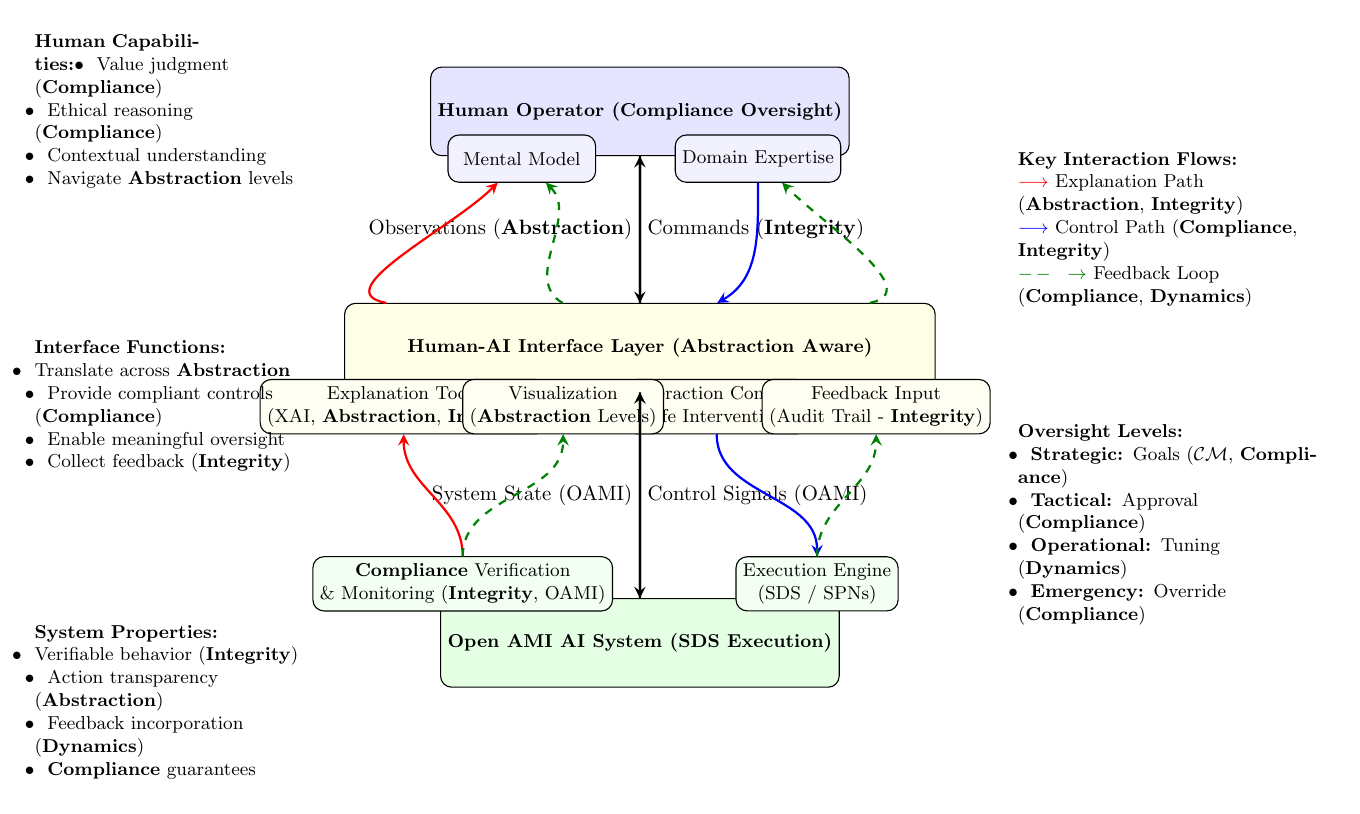
\begin{tikzpicture}[
			scale=0.75,
			transform shape,
			node distance=2cm,
			block/.style={rectangle, draw, rounded corners, minimum width=3cm, minimum height=1.2cm, align=center, font=\small},
			humanblock/.style={rectangle, draw, fill=blue!10, rounded corners, minimum width=6cm, minimum height=1.5cm, align=center, font=\small},
			systemblock/.style={rectangle, draw, fill=green!10, rounded corners, minimum width=6cm, minimum height=1.5cm, align=center, font=\small},
			interface/.style={rectangle, draw, fill=yellow!10, rounded corners, minimum width=10cm, minimum height=1.5cm, align=center, font=\small},
			arrow/.style={-stealth, thick},
			component/.style={rectangle, draw, rounded corners, minimum width=2.5cm, minimum height=0.8cm, align=center, font=\small},
			note/.style={rectangle, draw=none, text width=4.5cm, align=left, font=\small}
			]
			
			% Human operator
			\node[humanblock] (human) at (0,5) {\textbf{Human Operator (\textbf{Compliance} Oversight)}};
			
			% Interface Layer
			\node[interface] (interface) at (0,1) {\textbf{Human-AI Interface Layer (\Abstraction\ Aware)}};
			
			% System
			\node[systemblock] (system) at (0,-4) {\textbf{Open AMI AI System (SDS Execution)}};
			
			% Human components
			\node[component, fill=blue!5] (mental) at (-2,4.2) {Mental Model};
			\node[component, fill=blue!5] (expertise) at (2,4.2) {Domain Expertise};
			
			% Interface components - spaced out horizontally
			\node[component, fill=yellow!5] (explain) at (-4,0) {Explanation Tools\\(XAI, \Abstraction, \Integrity)};
			\node[component, fill=yellow!5] (interact) at (1.3,0) {Interaction Controls\\(Safe Interventions)};
			\node[component, fill=yellow!5] (vis) at (-1.3,0) {Visualization\\(\Abstraction\ Levels)};
			\node[component, fill=yellow!5] (feedback) at (4,0) {Feedback Input\\(Audit Trail - \Integrity)};
			
			% System components
			\node[component, fill=green!5] (align) at (-3,-3) {\textbf{Compliance} Verification\\\& Monitoring (\Integrity, OAMI)};
			\node[component, fill=green!5] (exec) at (3,-3) {Execution Engine\\(SDS / SPNs)};
			
			% Connections
			\draw[arrow] (human) to[out=270,in=90] node[right, midway] {Commands (\Integrity)} node[left, midway] {Observations (\Abstraction)} (interface);
			\draw[arrow] (interface) to[out=270,in=90] node[right, midway] {Control Signals (OAMI)} node[left, midway] {System State (OAMI)} (system);
			
			\draw[arrow] (system) to[out=90,in=270] (interface); % State Feedback
			\draw[arrow] (interface) to[out=90,in=270] (human); % Observation Feedback
			
			% Explanation flow (key path) with bends
			\draw[arrow, red, thick] (align) to[out=90,in=270] (explain);
			\draw[arrow, red, thick] (interface) to[out=170,in=225] (mental);
			
			% Control flow (key path) with bends
			\draw[arrow, blue, thick] (expertise) to[out=270,in=30] (interface);
			\draw[arrow, blue, thick] (interact) to[out=270,in=90] (exec);
			
			% Feedback loop with bends
			\draw[arrow, green!50!black, dashed] (exec) to[out=90,in=270] (feedback);
			\draw[arrow, green!50!black, dashed] (interface) to[out=11,in=315] (expertise);
			
			% Visualization connection with bends
			\draw[arrow, green!50!black, dashed] (align) to[out=90,in=270] (vis);
			\draw[arrow, green!50!black, dashed] (interface) to[out=150,in=315] (mental);
			
			% Notes - using manual list format
			\node[note] at (-8,5) {
				\textbf{Human Capabilities:}
				~~\llap{$\bullet$~~}Value judgment (\textbf{Compliance})\\
				~~\llap{$\bullet$~~}Ethical reasoning (\textbf{Compliance})\\
				~~\llap{$\bullet$~~}Contextual understanding\\
				~~\llap{$\bullet$~~}Navigate \Abstraction\ levels
			};
			
			\node[note] at (-8,0) {
				\textbf{Interface Functions:}
				~~\llap{$\bullet$~~}Translate across \Abstraction\\
				~~\llap{$\bullet$~~}Provide compliant controls (\textbf{Compliance})\\
				~~\llap{$\bullet$~~}Enable meaningful oversight\\
				~~\llap{$\bullet$~~}Collect feedback (\Integrity)
			};
			
			\node[note] at (-8,-5) {
				\textbf{System Properties:}
				~~\llap{$\bullet$~~}Verifiable behavior (\Integrity)\\
				~~\llap{$\bullet$~~}Action transparency (\Abstraction)\\
				~~\llap{$\bullet$~~}Feedback incorporation (\Dynamics)\\
				~~\llap{$\bullet$~~}\textbf{Compliance} guarantees
			};
			
			% Legend - using manual list format
			\node[note, text width=5.2cm] at (9,3) {
				\textbf{Key Interaction Flows:}\\
				\textcolor{red}{$\longrightarrow$} Explanation Path (\Abstraction, \Integrity)\\
				\textcolor{blue}{$\longrightarrow$} Control Path (\textbf{Compliance}, \Integrity)\\
				\textcolor{green!50!black}{$-\,-\!\rightarrow$} Feedback Loop (\textbf{Compliance}, \Dynamics)
			};
			
			% Legend - using manual list format
			\node[note, text width=5.2cm] at (9,-2) {
				\textbf{Oversight Levels:}\\
				~~\llap{$\bullet$~~}\textbf{Strategic:} Goals ($\mathcal{CM}$, \textbf{Compliance})\\
				~~\llap{$\bullet$~~}\textbf{Tactical:} Approval (\textbf{Compliance})\\
				~~\llap{$\bullet$~~}\textbf{Operational:} Tuning (\Dynamics)\\
				~~\llap{$\bullet$~~}\textbf{Emergency:} Override (\textbf{Compliance})
			};
			
		\end{tikzpicture}
		\caption[Human-AI Oversight Architecture]{Human-AI Oversight and Interaction Architecture. Enables human \textbf{Compliance} oversight via an \Abstraction-aware interface, relying on system \Integrity\ (SDS, OAMI) for trustworthy information exchange and control. Explanations leverage XAI tools and \Abstraction\ navigation; controls respect \textbf{Compliance} rules ($\mathcal{CM}$); feedback influences system \Dynamics.}
		\label{fig:human-oversight}
	\end{figure}
	
	\section{Limitations and Future Research Directions} % Corrected Section Title and Numbering
	\label{sec:5-8} % Adjusted label
	
	Addressing limitations in ensuring compliance for complex AI is ongoing.
	
	\subsection{Known Limitations} % Corrected Section Title and Numbering
	\label{sec:5-8-1} % Adjusted label
	
	\begin{itemize}
		\item \textbf{Value Specification Completeness/Nuance:} Capturing complex ethics in $\mathcal{CM}$ across \Abstraction\ levels is hard \citep{Kovac2025SpecGaming}.
		\item \textbf{Verification Scalability:} Formally verifying complex systems against $\mathcal{CM}$ (\textbf{Compliance}) with \Integrity\ is computationally demanding \citep{Peng2025ZKMLSurvey}.
		\item \textbf{Competing Values/Trade-offs:} Principled resolution of $\mathcal{CM}$ conflicts ($\mathcal{P}_{\text{conflict}}$) is difficult \citep{Sekrst2024Guardrails}.
		\item \textbf{Human Oversight Effectiveness:} Ensuring operators effectively use \Abstraction\ tools and manage complex \Dynamics\ under pressure.
		\item \textbf{Dynamic Environment Adaptation:} Guaranteeing continuous \textbf{Compliance} during adaptation (\Dynamics) requires robust re-verification and handling of distribution shifts \citep{AdditionalCitationRef53}.
		\item \textbf{Regulatory Evolution:} Requires efficient $\mathcal{CM}$ updates and re-verification (\Integrity\ of update process).
	\end{itemize}
	
	\subsection{Future Research Directions} % Corrected Section Title and Numbering
	\label{sec:5-8-2} % Adjusted label
	
	\begin{itemize}
		\item \textbf{Value Elicitation and Learning:} Better methods to elicit values for $\mathcal{CM}$, potentially learning constraints with \Integrity.
		\item \textbf{Scalable and Approximate Verification:} Efficient formal/statistical techniques for large-scale \textbf{Compliance}/\Integrity\ verification.
		\item \textbf{Dynamic Compliance Adaptation:} Mechanisms for safe adaptation of \textbf{Compliance} strategies based on context/\Dynamics.
		\item \textbf{Principled Conflict Resolution Frameworks:} Sophisticated formalisms/algorithms for executing $\mathcal{P}_{\text{conflict}}$ \citep{Sekrst2024Guardrails}.
		\item \textbf{Enhanced Human-AI Oversight Interfaces:} Better tools leveraging \Abstraction, visualization, AI-assist for managing complexity/\Dynamics.
		\item \textbf{Automated Regulatory Mapping and Auditing:} Tools for translating regulations to $\mathcal{CM}$ and generating \Integrity-proven compliance reports.
	\end{itemize}
	Figure~\ref{fig:research-roadmap} outlines a potential roadmap.
	
	\begin{figure}[ht]
		\centering
		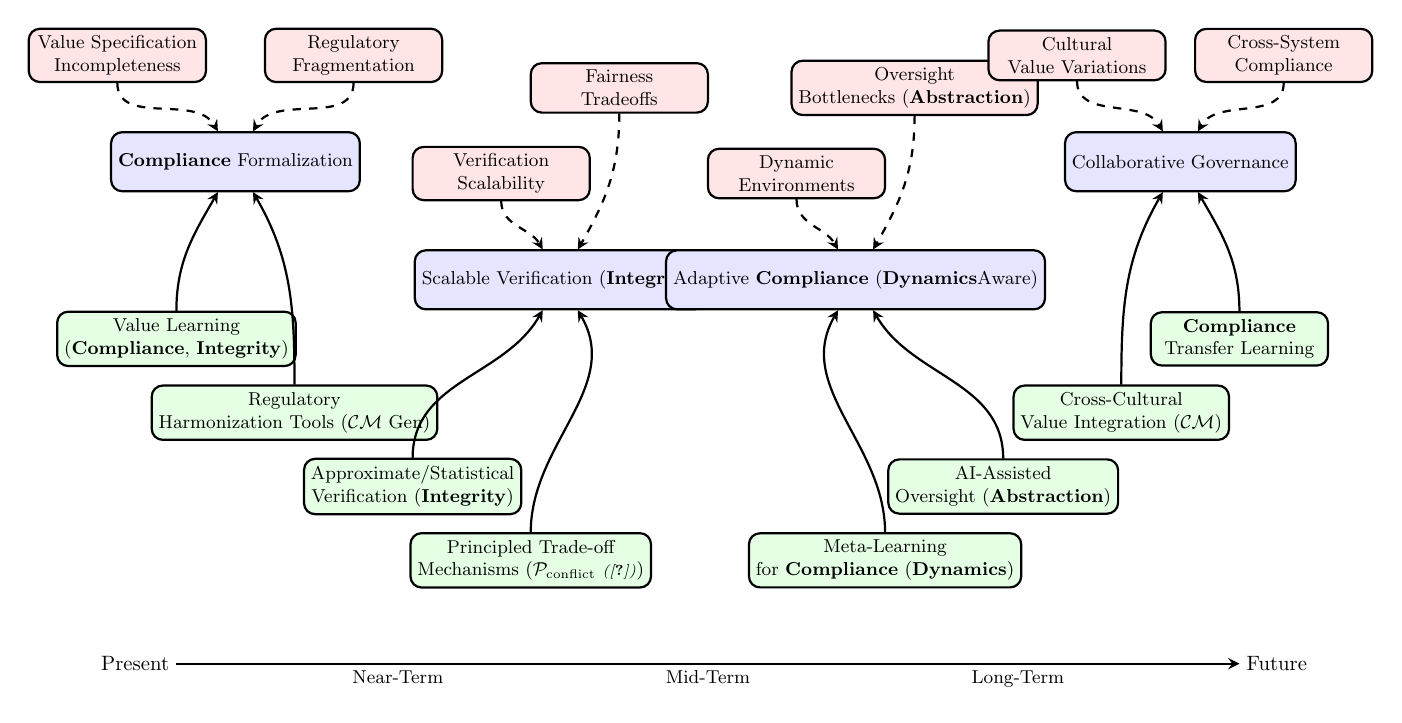
\begin{tikzpicture}[
			scale=0.75,
			transform shape,
			timeline/.style={draw, thick, -stealth},
			milestone/.style={circle, draw, thick, minimum size=0.6cm, font=\small},
			phase/.style={rectangle, rounded corners, draw, thick, fill=blue!10, minimum width=2.5cm, minimum height=1cm, align=center, font=\small},
			challenge/.style={rectangle, rounded corners, draw, thick, fill=red!10, minimum width=3cm, minimum height=0.8cm, align=center, font=\small},
			approach/.style={rectangle, rounded corners, draw, thick, fill=green!10, minimum width=3cm, minimum height=0.8cm, align=center, font=\small},
			arrow/.style={-stealth, thick},
			dasharrow/.style={-stealth, thick, dashed}
			]
			
			% Timeline
			\draw[timeline] (-9,-7) -- (9,-7);
			\node[left] at (-9,-7) {Present};
			\node[right] at (9,-7) {Future};
			
			% Phases
			\node[phase] (p1) at (-8,1.5) {\textbf{Compliance} Formalization};
			\node[phase] (p2) at (-2.5, -.5) {Scalable Verification (\Integrity)};
			\node[phase] (p3) at (2.5,-.5) {Adaptive \textbf{Compliance} (\Dynamics Aware)};
			\node[phase] (p4) at (8,1.5) {Collaborative Governance};
			
			% Challenges (above) - staggered vertically to avoid overlap
			\node[challenge] (c1) at (-10,3.3) {Value Specification\\Incompleteness};
			\node[challenge] (c2) at (-6,3.3) {Regulatory\\Fragmentation};
			\node[challenge] (c3) at (-3.5,1.3) {Verification\\Scalability};
			\node[challenge] (c4) at (-1.5,2.75) {Fairness\\Tradeoffs};
			\node[challenge] (c5) at (1.5,1.3) {Dynamic\\Environments};
			\node[challenge] (c6) at (3.5,2.75) {Oversight\\Bottlenecks (\Abstraction)};
			\node[challenge] (c7) at (6.25,3.3) {Cultural\\Value Variations};
			\node[challenge] (c8) at (9.75,3.3) {Cross-System\\Compliance};
			
			% Connect challenges to phases with bends
			\draw[dasharrow] (c1) to[out=270,in=120] (p1);
			\draw[dasharrow] (c2) to[out=270,in=60] (p1);
			\draw[dasharrow] (c3) to[out=270,in=120] (p2);
			\draw[dasharrow] (c4) to[out=270,in=60] (p2);
			\draw[dasharrow] (c5) to[out=270,in=120] (p3);
			\draw[dasharrow] (c6) to[out=270,in=60] (p3);
			\draw[dasharrow] (c7) to[out=270,in=120] (p4);
			\draw[dasharrow] (c8) to[out=270,in=60] (p4);
			
			% Approaches (below) - staggered vertically to avoid overlap
			\node[approach] (a1) at (-9,-1.5) {Value Learning\\(\textbf{Compliance}, \Integrity)};
			\node[approach] (a2) at (-7,-2.75) {Regulatory\\Harmonization Tools ($\mathcal{CM}$ Gen)};
			\node[approach] (a3) at (-5,-4) {Approximate/Statistical\\Verification (\Integrity)};
			\node[approach] (a4) at (-3,-5.25) {Principled Trade-off\\Mechanisms ($\mathcal{P}_{\text{conflict}}$ \citep{Sekrst2024Guardrails})};
			\node[approach] (a5) at (3,-5.25) {Meta-Learning\\for \textbf{Compliance} (\Dynamics)};
			\node[approach] (a6) at (5.,-4) {AI-Assisted\\Oversight (\Abstraction)};
			\node[approach] (a7) at (7,-2.75) {Cross-Cultural\\Value Integration ($\mathcal{CM}$)};
			\node[approach] (a8) at (9,-1.5) {\textbf{Compliance}\\Transfer Learning};
			
			% Connect approaches to phases with bends
			\draw[arrow] (a1) to[out=90,in=240] (p1);
			\draw[arrow] (a2) to[out=90,in=300] (p1);
			\draw[arrow] (a3) to[out=90,in=240] (p2);
			\draw[arrow] (a4) to[out=90,in=300] (p2);
			\draw[arrow] (a5) to[out=90,in=240] (p3);
			\draw[arrow] (a6) to[out=90,in=300] (p3);
			\draw[arrow] (a7) to[out=90,in=240] (p4);
			\draw[arrow] (a8) to[out=90,in=300] (p4);
			
			% Period labels
			\node[below, font=\small] at (-5.25,-7) {Near-Term};
			\node[below, font=\small] at (0,-7) {Mid-Term};
			\node[below, font=\small] at (5.25,-7) {Long-Term};
			
		\end{tikzpicture}
		\caption[Research Roadmap for Open AMI Compliance]{Research Roadmap for Open AMI Compliance and Trustworthiness. Outlines a progressive research agenda addressing current limitations through phases: Formalization Refinement, Scalable Verification (\Integrity), Adaptive Alignment (\Dynamics), and Collaborative Governance. Each phase targets specific challenges (top) with potential research approaches (bottom), aiming to enhance the framework's ability to ensure \textbf{Compliance} in complex systems across various \Abstraction\ levels.}
		\label{fig:research-roadmap}
	\end{figure}
	
	\section{Conclusion: Governance for Trustworthy AI/ML} % Corrected Section Title and Numbering
	\label{sec:5-9} % Adjusted label
	
	The \textbf{Compliance} framework detailed in this chapter constitutes the primary governance mechanism of the Open AMI architecture. It provides the essential capabilities for defining (\textbf{Compliance} Manifest, $\mathcal{CM}$), verifying, and enforcing the ethical, legal, safety, and operational rules necessary for trustworthy AI/ML systems. By formalizing requirements in $\mathcal{CM}$ (addressing the specification challenge \citep{Kovac2025SpecGaming}), integrating verification and enforcement throughout the system lifecycle (leveraging the SDS), enabling meaningful human oversight (supported by research in ethical AI practice \citep{Crossing_Principle_Practice_Gap_2024}), and providing principled methods for conflict resolution ($\mathcal{P}_{\text{conflict}}$ \citep{Sekrst2024Guardrails}), it offers a comprehensive approach to guiding AI behavior, aligning with established principles like Constitutional AI \citep{Bai2022ConstitutionalAI}.
	
	Critically, this compliance framework does not operate in isolation but interacts deeply with the other core pillars. It relies fundamentally on the verifiable \Integrity\ provided by the SDS for its monitoring and enforcement functions. It operates across multiple levels of \Abstraction, allowing constraints from $\mathcal{CM}$ to be specified and verified appropriately. Furthermore, it must account for and manage system \Dynamics, ensuring compliance is maintained even as systems learn and adapt \citep{Wang2024ContinualLearningSurvey}, guided by the Governance Layer. This holistic, integrated approach enables Open AMI systems, including those employing sophisticated ML techniques (Chapter~\ref{ch:machine_learning}), to pursue advanced capabilities while remaining verifiably aligned with human values and societal norms.
	
		\appendix
	
	\chapter{Open AMI (OAMI) Protocol Specification}
	\label{app:protocol_spec}
	
	\section{Abstract}
	
	This appendix specifies the \textbf{Open AMI (OAMI) Protocol}, the standard communication layer designed for components operating within the Open AMI framework. OAMI builds upon concepts found in modern agent communication protocols, such as Google's Agent2Agent (A2A) \citep{A2A_README}, extending them to meet the specific requirements of trustworthy AI/ML systems developed under Open AMI principles. It defines standardized methods for task execution and tracking, status monitoring, and crucially, structured knowledge sharing and collaboration, potentially leveraging Knowledge Graphs (KGs). The protocol facilitates interactions like KG querying (e.g., using GraphQL), verifiable updates, and real-time subscriptions. It incorporates mechanisms for enforcing \Compliance\ policies (referencing $\mathcal{CM}$), ensuring message and data \Integrity\ (leveraging SDS capabilities), tracking provenance, managing uncertainty, and supporting operations across different levels of \Abstraction\ and system \Dynamics. OAMI provides the secure and verifiable communication substrate necessary for complex, collaborative, and compliant operations within an Open AMI system, addressing the need for robust interoperability noted in agent frameworks and multi-agent systems \citep{AdditionalCitationRef52}.
	
	\section{Motivation and Relationship to A2A}
	\label{app:oami_motivation}
	
	While protocols like A2A \citep{A2A_README} offer a foundation for basic agent interoperability (task definition, status tracking, message exchange), the goals of the Open AMI framework necessitate extensions to handle verifiable computation, compliant learning processes, sophisticated knowledge sharing, and rigorous governance oversight. Specifically, Open AMI requires protocol-level features that support:
	\begin{itemize}
		\item End-to-end cryptographic \Integrity\ guarantees for messages, exchanged data, and potentially state transitions communicated via the protocol, facilitated by the SDS. This moves beyond basic transport security to verifiable payloads, potentially using signatures or proofs \citep{Peng2025ZKMLSurvey}.
		\item The embedding of \textbf{Compliance} context (e.g., purpose of request, applicable $\mathcal{CM}$ policies) and verification status information directly within interactions, enabling context-aware policy enforcement \citep{Sekrst2024Guardrails}.
		\item Standardized methods for interacting with structured knowledge representations, such as Knowledge Graphs, to enable advanced reasoning and collaborative learning among components, ensuring knowledge \Integrity.
		\item Mechanisms to facilitate operations across different levels of \Abstraction\ (e.g., requesting information at a specific level of detail).
		\item Features supporting the monitoring and control of system \Dynamics\ (e.g., streaming status updates, reporting resource usage).
	\end{itemize}
	OAMI adopts core A2A concepts like task lifecycles, component descriptors, and streaming via Server-Sent Events (SSE). However, it extends these with specific methods (especially for knowledge graphs), parameters (e.g., for compliance context, integrity proofs, certainty levels), and data structures tailored to the four Open AMI pillars (\Compliance, \Integrity, \Abstraction, \Dynamics). The goal is to provide a richer, more secure, and more verifiable communication standard suitable for trustworthy advanced AI/ML systems, addressing limitations seen in simpler agent communication paradigms \citep{AdditionalCitationRef52}.
	
	\section{Core Concepts}
	\label{app:oami_concepts}
	
	\begin{description}
		\item[OAMI Component:] Any functional unit within an Open AMI system (e.g., an application running in an SPN, a Meta-Process, an external service gateway) that communicates using the OAMI protocol.
		\item[Component Descriptor:] Standardized metadata describing an OAMI Component. Includes identity, OAMI endpoint, authentication requirements, declared capabilities (supported OAMI methods, KG query languages, supported \textbf{Compliance} checks, offered \Integrity\ mechanisms). Its own \Integrity\ must be verifiable.
		\item[OAMI Server:] An OAMI Component that implements and exposes OAMI methods at a specific network endpoint, secured by the SDS.
		\item[OAMI Client:] An OAMI Component that initiates OAMI requests to an OAMI Server.
		\item[Task:] A unit of work managed via the protocol, identified by a unique \texttt{taskId}. Tasks progress through states (e.g., \texttt{submitted}, \texttt{running}, \texttt{completed}, \texttt{failed}, \texttt{cancelled}). Task state transitions and associated Artifacts MUST be logged by the SDS with verifiable \Integrity.
		\item[Message:] A single turn of communication within a Task context. Contains \texttt{Parts}, identifies sender's role, includes metadata for \textbf{Compliance}/\Integrity.
		\item[Part:] A unit of content within a Message (e.g., \texttt{TextPart}, \texttt{FilePart}, \texttt{DataPart}). \Integrity\ verifiable via hashes/signatures in metadata.
		\item[Artifact:] An output generated by a Task, containing \texttt{Parts}. MUST include metadata detailing origin, processing steps, and an \Integrity\ proof (e.g., signature/hash generated by the originating SPN, potentially referencing a PoL proof \citep{Jia2021ProofOfLearning}).
		\item[Streaming:] Real-time updates via Server-Sent Events (SSE) for specific methods (e.g., \texttt{tasks/sendSubscribe}, \texttt{knowledge/subscribe}), requiring declared capability. Stream \Integrity\ protected by underlying secure channel.
		\item[Knowledge Graph (KG):] Structured knowledge potentially managed by OAMI Components (in SPNs). OAMI defines standard interaction methods ensuring \Integrity\ and \textbf{Compliance}.
	\end{description}
	
	\section{Protocol Transport and Structure}
	\label{app:oami_transport_structure}
	
	\begin{itemize}
		\item \textbf{Transport:} Secure HTTPS with mutual TLS (mTLS) is REQUIRED, managed by the SDS infrastructure, ensuring channel confidentiality, authenticity, and baseline message \Integrity.
		\item \textbf{Structure:} Adheres to JSON-RPC 2.0 specification. Requests include \texttt{jsonrpc: "2.0"}, \texttt{method}, \texttt{params}, \texttt{id}. Responses include \texttt{jsonrpc: "2.0"}, \texttt{result} or \texttt{error}, \texttt{id}.
		\item \textbf{Security and Compliance Context (\texttt{metadata}):} A standard field within \texttt{params} carries supplementary context crucial for Open AMI:
		\begin{itemize}
			\item Security tokens (for authorization).
			\item \textbf{Compliance} context (e.g., task purpose specification referencing $\mathcal{CM}$, data usage constraints, required fairness level).
			\item Request-level \Integrity\ proofs (e.g., signature covering parameters).
			\item Provenance information (data origin ID, process ID).
			\item Desired \Abstraction\ level for response.
			\item Relevant \Dynamics\ context (e.g., priority, deadline).
		\end{itemize}
		Specific content depends on the method and $\mathcal{CM}$ policies. Servers MUST validate this metadata (\textbf{Compliance}, \Integrity).
	\end{itemize}
	
	\section{OAMI Protocol Methods}
	\label{app:oami_methods}
	
	\subsection{Task Management Methods}
	\label{app:oami_task_mgmt}
	
	Manage units of work; state changes/artifacts logged with verifiable \Integrity\ by SDS.
	
	\subsubsection{\texttt{tasks/send}}
	\label{app:oami_tasks_send}
	\begin{description}
		\item[Purpose:] Initiates a new task or sends subsequent message. For request-response interactions.
		\item[Params:]
		\begin{itemize} \itemsep0em
			\item \texttt{taskId} (string | null): ID of existing task, or null/omitted for new task.
			\item \texttt{message} (\texttt{Message}, required): Payload with \texttt{Parts}.
			\item \texttt{sessionId} (string | null): Optional session identifier.
			\item \texttt{metadata} (object | null): Security tokens, \textbf{Compliance} context (purpose), \Integrity\ proofs.
		\end{itemize}
		\item[Result:] Final \texttt{Task} object upon completion (\texttt{status: "completed"}), including final \texttt{artifacts} with \Integrity\ proofs.
		\item[Notes:] Server (SPN/Meta-Process) MUST verify \Integrity\ of message parts, authorization, and \textbf{Compliance} based on \texttt{metadata} and $\mathcal{CM}$ before processing. Task creation/message receipt logged (\Integrity).
	\end{description}
	
	\subsubsection{\texttt{tasks/sendSubscribe}}
	\label{app:oami_tasks_sendsubscribe}
	\begin{description}
		\item[Purpose:] Initiates/continues task, subscribing client to real-time SSE updates (status, intermediate artifacts). Requires server `streaming` capability.
		\item[Params:] Same as \texttt{tasks/send}.
		\item[Response (Initial):] HTTP 200 OK, \texttt{Content-Type: text/event-stream}. Initial errors are standard HTTP/JSON-RPC errors.
		\item[Response (Streaming):] SSE stream with JSON-RPC Response objects in `data`. Events like \texttt{TaskStatusUpdateEvent} or \texttt{TaskArtifactUpdateEvent}. Stream \Integrity\ from TLS. Event data \Integrity\ verifiable by client (e.g., signed artifacts). Monitors task \Dynamics.
	\end{description}
	
	\subsubsection{\texttt{tasks/getStatus}}
	\label{app:oami_tasks_getstatus}
	\begin{description}
		\item[Purpose:] Retrieves current status/details of a specific task.
		\item[Params:] \texttt{taskId} (string, required).
		\item[Result:] Current \texttt{Task} object.
		\item[Notes:] Requires authorization (\textbf{Compliance} check) referencing $\mathcal{CM}$.
	\end{description}
	
	\subsubsection{\texttt{tasks/cancel}}
	\label{app:oami_tasks_cancel}
	\begin{description}
		\item[Purpose:] Requests cancellation of an ongoing task. Server determines graceful stop.
		\item[Params:]
		\begin{itemize} \itemsep0em
			\item \texttt{taskId} (string, required).
			\item \texttt{justification} (string | null): Reason for audit log.
			\item \texttt{metadata} (object | null): Authorization context.
		\end{itemize}
		\item[Result:] Confirmation object, e.g., \texttt{\{ success: true, finalStatus: "cancelling" | "cancelled" \}}.
		\item[Notes:] Requires authorization (\textbf{Compliance}). Request and state change logged with verifiable \Integrity.
	\end{description}
	
	\subsection{Knowledge Graph Methods}
	\label{app:oami_kg_methods}
	
	Interact with KGs hosted by OAMI Components (SPNs). Requires server capability declaration. Ensures \Integrity\ and \textbf{Compliance} of knowledge operations.
	
	\subsubsection{\texttt{knowledge/query}}
	\label{app:oami_kg_query}
	\begin{description}
		\item[Purpose:] Query the Knowledge Graph.
		\item[Params (\texttt{KnowledgeQueryParams}):]
		\begin{itemize} \itemsep0em
			\item \texttt{query} (string, required): Query string (e.g., GraphQL, SPARQL).
			\item \texttt{queryLanguage} (string, required): Specifies language. MUST be supported by server.
			\item \texttt{variables} (object | null): Optional query variables.
			\item \texttt{taskId} (string | null): Optional task context link.
			\item \texttt{metadata} (object | null): Security token, query purpose (\textbf{Compliance} check against $\mathcal{CM}$), required \Abstraction\ level, request \Integrity\ proof.
			\item \texttt{requiredCertainty} (number | null): Optional filter [0.0, 1.0] for result certainty (\Integrity\ metadata).
			\item \texttt{maxAgeSeconds} (integer | null): Optional filter for data freshness (provenance \Integrity).
		\end{itemize}
		\item[Result (\texttt{KnowledgeQueryResponseResult}):]
		\begin{itemize} \itemsep0em
			\item \texttt{data} (object | array | null): Query results.
			\item \texttt{queryMetadata} (object | null): Execution info, timing, sources consulted, aggregate certainty/provenance, data \Integrity\ status.
		\end{itemize}
		\item[Errors:] Standard JSON-RPC, \texttt{-32010 KnowledgeQueryError}, \texttt{-32014 UnsupportedQueryLanguageError}, \texttt{-32013 AlignmentViolationError} (violates $\mathcal{CM}$ data access policy), \texttt{-32015 IntegrityVerificationError} (underlying data integrity fail). Server MUST check \textbf{Compliance} based on metadata/\textbf{Compliance}.
	\end{description}
	
	\subsubsection{\texttt{knowledge/update}}
	\label{app:oami_kg_update}
	\begin{description}
		\item[Purpose:] Propose changes (add/remove) to the KG. Server MUST verify changes for \textbf{Compliance} and \Integrity\ before applying (potentially asynchronously or requiring approval).
		\item[Params (\texttt{KnowledgeUpdateParams}):]
		\begin{itemize} \itemsep0em
			\item \texttt{mutations} (array[\texttt{KnowledgeGraphPatch}], required, minItems: 1): Proposed changes (\texttt{add}/\texttt{remove} \texttt{KGStatement}). Statements include provenance/\Integrity\ info.
			\item \texttt{taskId} (string | null): Optional task context link.
			\item \texttt{sourceComponentId} (string, required): Authenticated ID of proposer (provenance/\Integrity).
			\item \texttt{justification} (string, required): Reason for update (auditability/\textbf{Compliance}).
			\item \texttt{metadata} (object | null): Security context, additional \textbf{Compliance} context or pre-verification evidence (\Integrity\ proof).
		\end{itemize}
		\item[Result (\texttt{KnowledgeUpdateResponseResult}):]
		\begin{itemize} \itemsep0em
			\item \texttt{success} (boolean): Request syntactically valid and accepted for processing/review.
			\item \texttt{verificationStatus} (string, required): Detailed status, e.g., \texttt{"VerifiedAndApplied"}, \texttt{"PendingHumanReview"}, \texttt{"RejectedAlignmentViolation"}, \texttt{"RejectedIntegrityFailure"}. Feedback on \textbf{Compliance}/\Integrity\ checks.
			\item \texttt{verificationDetails} (string | null): Optional explanation.
			\item \texttt{statementsAffected} (integer | null): Estimate of affected statements.
			\item \texttt{affectedIds} (array[string] | null): URIs/IDs potentially affected.
		\end{itemize}
		\item[Errors:] Standard JSON-RPC, \texttt{-32011 KnowledgeUpdateError}, \texttt{-32013 AlignmentViolationError}. Entire update attempt logged with verifiable \Integrity.
	\end{description}
	
	\subsubsection{\texttt{knowledge/subscribe}}
	\label{app:oami_kg_subscribe}
	\begin{description}
		\item[Purpose:] Subscribe to real-time KG changes matching a query pattern. Requires server `streaming` and `knowledgeGraph` capabilities. Monitors knowledge \Dynamics.
		\item[Params (\texttt{KnowledgeSubscribeParams}):]
		\begin{itemize} \itemsep0em
			\item \texttt{subscriptionQuery} (string, required): Query defining pattern of interest (e.g., GraphQL subscription).
			\item \texttt{queryLanguage} (string, required): Language of query. MUST be supported.
			\item \texttt{variables} (object | null): Optional query variables.
			\item \texttt{taskId} (string | null): Optional task context link.
			\item \texttt{metadata} (object | null): Security/\textbf{Compliance} context for establishing subscription (authorization, purpose).
		\end{itemize}
		\item[Response (Initial):] HTTP 200 OK, \texttt{Content-Type: text/event-stream}. Setup errors returned before stream starts. Requires authorization (\textbf{Compliance}).
		\item[Response (Streaming):] SSE stream. Event `data` contains JSON-RPC Response object. \texttt{result} holds \texttt{KnowledgeSubscriptionEvent} detailing the change (\texttt{changeId}, \texttt{timestamp}, \texttt{operationType}, changed \texttt{statement} with certainty/provenance/\Integrity\ hash). Stream \Integrity\ from TLS. Client should verify event data \Integrity.
		\item[Errors:] Standard JSON-RPC, \texttt{-32012 KnowledgeSubscriptionError}, \texttt{-32014 UnsupportedQueryLanguageError}, \texttt{-32013 AlignmentViolationError} (subscription violates $\mathcal{CM}$ policy). Stream can transmit errors.
	\end{description}
	
	\section{Core Knowledge Data Structures}
	\label{app:oami_kg_structures}
	
	Conceptual JSON-like structures for information content, focusing on pillar support. Formal schema definition (e.g., JSON Schema) is needed for implementation.
	
	\begin{description}
		\item[\texttt{KGSubject}:] \texttt{\{ id: string (URI), type?: string (URI) \}}
		\item[\texttt{KGPredicate}:] \texttt{\{ id: string (URI) \}}
		\item[\texttt{KGObject}:] \texttt{\{ id?: string (URI), value?: any (literal), type?: string (URI), lang?: string \}}
		\item[\texttt{KGStatement}:] \texttt{\{ subject: KGSubject, predicate: KGPredicate, object: KGObject, graph?: string (URI), certainty?: number [0-1], provenance: \{ sourceComponentId: string, timestamp: datetime, method: string, integrityProof: string (hash/signature) \} \}}. Certainty and provenance crucial for \Integrity.
		\item[\texttt{PatchOperationType}:] Enum: \texttt{"add"} | \texttt{"remove"}.
		\item[\texttt{KnowledgeGraphPatch}:] \texttt{\{ op: PatchOperationType, statement: KGStatement \}}. Used in \texttt{knowledge/update}.
	\end{description}
	
	\section{Error Handling}
	\label{app:oami_errors}
	
	OAMI defines specific error codes (-32000 to -32099 range) for granular feedback related to trustworthiness pillars:
	
	\begin{description} \itemsep0em
		\item[\texttt{-32010 KnowledgeQueryError}:] General KG query failure.
		\item[\texttt{-32011 KnowledgeUpdateError}:] KG update rejected (schema, conflict, etc.).
		\item[\texttt{-32012 KnowledgeSubscriptionError}:] KG subscription failure.
		\item[\texttt{-32013 AlignmentViolationError}:] Operation blocked by \textbf{Compliance} policy ($\mathcal{CM}$). `data` may contain details.
		\item[\texttt{-32014 UnsupportedQueryLanguageError}:] Query language not supported.
		\item[\texttt{-32015 IntegrityVerificationError}:] Request/data failed \Integrity\ check (bad signature/hash).
		\item[\texttt{-32016 ComplianceCheckError}:] Error occurred during \textbf{Compliance} check execution.
		\item[\texttt{-32017 TaskNotFound}:] Invalid \texttt{taskId} or unauthorized access.
		\item[\texttt{-32018 AbstractionLevelError}:] Operation requested at unsupported/inappropriate \Abstraction\ level.
		\item[\texttt{-32019 DynamicsControlError}:] Command related to system \Dynamics\ failed/rejected.
	\end{description}
	Error responses SHOULD include informative `message` strings and potentially structured `data` fields, respecting security/privacy.
	
	\section{Integration with Open AMI Pillars}
	\label{app:oami_pillar_integration_details} % Changed label to be more specific
	
	OAMI design explicitly supports the four pillars:
	
	\begin{itemize}
		\item \textbf{\Compliance}: Enforced via checks linked to $\mathcal{CM}$ during method execution (validating purpose/context in \texttt{metadata}, checking data access policies for KG methods, handling \texttt{AlignmentViolationError}). Provenance tracking supports \textbf{Compliance}.
		\item \textbf{\Integrity}: Ensured via mandatory secure transport (mTLS managed by SDS), authentication, optional payload signing, explicit provenance/\Integrity\ fields in data structures (\texttt{KGStatement}, Artifacts, CSTs communicated via messages), verifiable logging requirements (SDS), specific error codes (\texttt{IntegrityVerificationError}).
		\item \textbf{\Abstraction}: Supported by allowing requests to specify desired levels of detail (\texttt{metadata}), enabling KG queries retrieving info at specific conceptual levels, component descriptors declaring abstraction capabilities.
		\item \textbf{\Dynamics}: Facilitated by real-time streaming (\texttt{tasks/sendSubscribe}, \texttt{knowledge/subscribe}). Status updates and shared knowledge support coordinated dynamic adjustments. Monitoring data related to \Dynamics\ exchanged via standard messages or dedicated methods.
	\end{itemize}
	
	\section{Interaction Flow Diagrams}
	\label{app:oami_flow_diagrams}
	
	Placeholders - diagrams to be generated using tools like PlantUML/Mermaid and included as PDFs.
	
	\subsection{Client-Server Knowledge Query}
	\label{app:oami_flow_client_server}
	
	\begin{figure}[H]
		\centering
		% Placeholder - Requires actual sequence diagram
		%\includegraphics[width=0.9\textwidth]{{sequence_client_server}.pdf}
		\caption{OAMI Protocol: Client-Server Knowledge Query Interaction Flow. Illustrates a client sending a `knowledge/query` request (including metadata for auth/\textbf{Compliance}) via secure OAMI/HTTPS, the server verifying \textbf{Compliance} and \Integrity, executing the query, and returning results with \Integrity\ metadata.}
		\label{fig:oami_client_server_flow}
	\end{figure}
	
	\subsection{Peer-to-Peer Knowledge Update Example}
	\label{app:oami_flow_peer_to_peer}
	
	\begin{figure}[H]
		\centering
		% Placeholder - Requires actual sequence diagram
		%\includegraphics[width=\textwidth]{{sequence_peer_to_peer}.pdf}
		\caption{OAMI Protocol: Peer-to-Peer Knowledge Update Example. Shows Component A proposing a KG change to Component B using `knowledge/update`. Component B authenticates A, verifies the update against $\mathcal{CM}$ (\textbf{Compliance}) and data \Integrity, applies the change if valid, logs (\Integrity), and returns status.}
		\label{fig:oami_peer_to_peer_flow}
	\end{figure}
	
	\section{Conclusion}
	\label{app:oami_conclusion}
	
	The Open AMI (OAMI) Protocol Specification defines a communication standard tailored for trustworthy, advanced AI/ML systems within the Open AMI framework. By extending A2A concepts with robust task management, powerful Knowledge Graph interaction (\Integrity, \textbf{Compliance}), and embedded mechanisms supporting all four pillars (\Compliance, \Integrity, \Abstraction, \Dynamics), OAMI enables secure, verifiable, and collaborative interactions managed by the SDS. It provides the essential communication fabric for complex, multi-component Open AMI systems designed to be both capable and demonstrably responsible. Future versions may refine error handling, add dynamic capability negotiation, or specify richer metadata formats.
	
		\chapter{Open AMI Simulation Subsystem (OASIM) Specification}
	\label{app:simulation_subsystem}
	
	\section{Introduction: Simulation for Grounding, Verification, and Embodiment}
	\label{app:oasim_intro}
	
	Developing robust and trustworthy AI systems, particularly those intended to interact with the physical world or requiring validation against physical laws, necessitates powerful simulation capabilities. The \textbf{Open AMI Simulation Subsystem (OASIM)} is specified here to fulfill this critical role within the Open AMI framework. OASIM functions as a specialized, potentially distributed service, accessible via the OAMI protocol (Appendix~\ref{app:protocol_spec}), typically operating within the secure execution environment provided by the Secure Distributed System (SDS, Chapter~\ref{ch:secure_distributed_system}).
	
	OASIM serves three primary functions crucial for trustworthy AI development, directly supporting the Open AMI pillars:
	\begin{enumerate}
		\item \textbf{Grounding Reasoning and Verification (\Integrity, \textbf{Compliance}):} Provides OAMI Components (e.g., ARUs in SPNs) with a capability to simulate physical scenarios or physics-based analogies with verifiable simulation \Integrity. This allows components to:
		\begin{itemize}
			\item Check physical plausibility of plans/actions against simulated physics.
			\item Predict physical consequences under known laws, potentially using techniques like Model Predictive Control \citep{Berg2025DigitalTwin}.
			\item Verify adherence to physical safety constraints (defined as part of \textbf{Compliance} in $\mathcal{CM}$).
			\item Execute/validate physics-inspired reasoning processes (Sec~\ref{sec:2-4-2}) for potentially higher \Integrity\ computation \citep{Physics-InspiredReasoning_Ref14, Physics-InspiredReasoning_Ref17}, aligning with research on physics-regulated AI \citep{Cao_PhyDRL_2024}.
		\end{itemize}
		\item \textbf{Supporting Embodied Agents (\Dynamics, \textbf{Compliance}):} Furnishes simulation infrastructure for training (RL), testing, evaluating, and planning for physically embodied OAMI agents (robots, vehicles). Enables creating digital twins for monitoring/prediction \citep{Li2025DigitalTwins, Berg2025DigitalTwin}, ensuring simulated behavior adheres to physical laws (\Integrity) and \textbf{Compliance} constraints (operational boundaries, force limits). Supports managing agent \Dynamics\ in simulation and addressing the sim-to-real gap \citep{Josifovski_SCDA_2025, Li2025DigitalTwins}.
		\item \textbf{Interoperability and Standardization (\Abstraction):} Ensures compatibility by adopting \textbf{Universal Scene Description (USD)} as the core standard for scene description, data exchange, and simulation state representation, enabling strong integration with platforms like \textbf{NVIDIA Omniverse}. USD facilitates managing scene complexity at different levels of \Abstraction.
	\end{enumerate}
	OASIM operates under Open AMI governance. Its operations must adhere to \textbf{Compliance} constraints (resource limits, permitted scenarios from $\mathcal{CM}$), ensure simulation \Integrity\ (verifiable physics, state data), support interactions at appropriate \Abstraction\ levels, and manage its own computational \Dynamics.
	
	\section{Subsystem Architecture}
	\label{app:oasim_architecture_section} % Changed label to be more specific
	
	OASIM has a modular, service-oriented architecture:
	
	\begin{figure}[H]
		\centering
		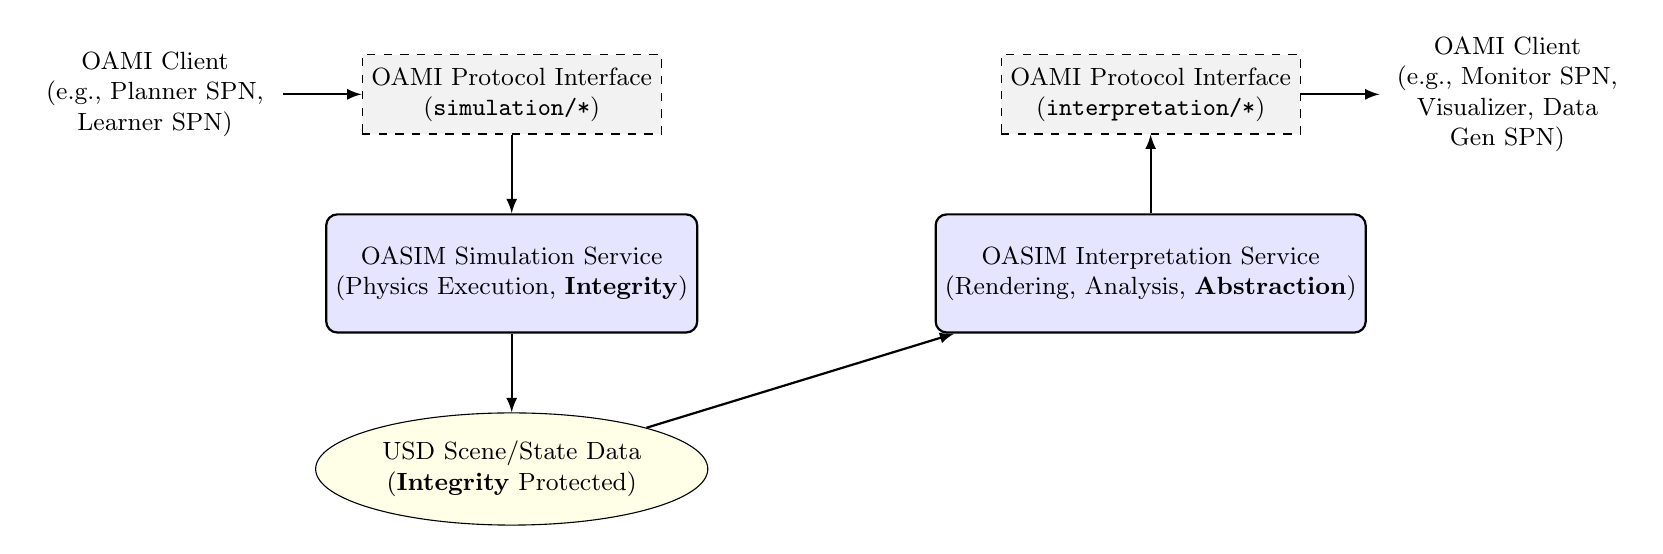
\begin{tikzpicture}[node distance=2cm, auto, >=latex,
			service/.style={rectangle, draw, thick, rounded corners, fill=blue!10, minimum width=3.5cm, minimum height=1.5cm, text centered, font=\small},
			protocol/.style={rectangle, draw, dashed, fill=gray!10, minimum width=3cm, minimum height=0.8cm, text centered, font=\small},
			data/.style={ellipse, draw, fill=yellow!10, minimum width=2.5cm, minimum height=1cm, text centered, font=\small},
			arrow/.style={->, thick}
			]
			\node[service] (sim_svc) {\makecell{OASIM Simulation Service\\(Physics Execution, \Integrity)}};
			\node[service, right=3cm of sim_svc] (interp_svc) {\makecell{OASIM Interpretation Service\\(Rendering, Analysis, \Abstraction)}};
			\node[protocol, above=1cm of sim_svc] (oami_in) {\makecell{OAMI Protocol Interface\\(\texttt{simulation/*})}};
			\node[protocol, above=1cm of interp_svc] (oami_out) {\makecell{OAMI Protocol Interface\\(\texttt{interpretation/*})}};
			\node[data, below=1cm of sim_svc] (usd_data) {\makecell{USD Scene/State Data\\(\Integrity\ Protected)}};
			
			\draw[arrow] (oami_in) -- (sim_svc);
			\draw[arrow] (sim_svc) -- (usd_data);
			\draw[arrow] (usd_data) -- (interp_svc);
			\draw[arrow] (interp_svc) -- (oami_out);
			
			
			\node[left=1cm of oami_in, text width=3cm, font=\small, align=center] (client_sim) {OAMI Client \\ (e.g., Planner SPN, \\ Learner SPN)};
			\draw[arrow] (client_sim) -- (oami_in);
			
			\node[right=1cm of oami_out, text width=3cm, font=\small, align=center] (client_interp) {OAMI Client \\ (e.g., Monitor SPN, \\ Visualizer, Data Gen SPN)};
			\draw[arrow] (oami_out) -- (client_interp);
			
		\end{tikzpicture}
		\caption{Conceptual OASIM Architecture. OAMI Components (SPNs) interact with OASIM services via OAMI. The Simulation Service executes physics with verifiable \Integrity, producing \Integrity-protected USD state. The Interpretation Service consumes USD for rendering, analysis, or sensor simulation, providing results at appropriate \Abstraction\ levels via OAMI.}
		\label{fig:OASIM_architecture}
	\end{figure}
	
	\begin{enumerate}
		\item \textbf{OASIM Simulation Service:} The core engine. Receives OAMI \texttt{simulation/*} requests, manages simulation instances, orchestrates pluggable physics solvers (potentially Omniverse backend), handles coupling, generates USD state data. MUST run within SDS to ensure simulation process \Integrity.
		\item \textbf{OASIM Interpretation Service:} Consumes USD simulation state. Provides higher-level functionalities via OAMI \texttt{interpretation/*} methods:
		\begin{itemize}
			\item \textbf{Rendering (\Abstraction):} Uses rendering engines (e.g., Omniverse RTX) for visualizations (images, video) from USD scenes. Supports different \Abstraction\ levels in visualization.
			\item \textbf{Analysis (\textbf{Compliance}, \Integrity):} Performs quantitative analysis (extract variables, check physical/\textbf{Compliance} constraints from $\mathcal{CM}$, statistics, event detection). Results MUST have verifiable \Integrity.
			\item \textbf{Sensor Simulation (\Integrity):} Generates realistic synthetic sensor data (camera, LiDAR, IMU) based on USD state and sensor models. Output data includes \Integrity\ metadata. Crucial for sim-to-real training \citep{Li2025DigitalTwins}.
		\end{itemize}
		May also run within SDS, utilizing dedicated hardware (GPUs). Results must maintain verifiable \Integrity.
	\end{enumerate}
	OAMI Components interact with OASIM via specified OAMI methods.
	
	\section{Simulation Service Specification}
	\label{app:oasim_sim_service_spec}
	
	\subsection{Pluggable Physics Solvers (\Integrity)}
	\label{app:oasim_physics_solvers}
	OASIM supports modular physics solvers, ensuring execution \Integrity:
	\begin{itemize}
		\item Standard Rigid/Soft Body Dynamics (e.g., PhysX 5 via Omniverse).
		\item Specialized solvers (CFD, FEA, particles). Solvers run within SPNs or trusted execution environments.
		\item Custom solvers for physics-based analogies \citep{Physics-InspiredReasoning_Ref14, Physics-InspiredReasoning_Ref17}.
	\end{itemize}
	Choice determined by \texttt{physicsConfig} in \texttt{simulation/setup}. Execution \Integrity\ verified or assured (e.g., via TEE attestation if solver runs in TEE-based SPN).
	
	\subsection{Multi-Scale Coupling (\Integrity, \Abstraction)}
	\label{app:oasim_multiscale}
	Supports coupling different physics solvers for multi-scale scenarios \citep{MultiScaleVis_Ref1, MultiScaleVis_Ref13}. Strategies specified in \texttt{physicsConfig}. Ensuring stable, accurate (\Integrity) coupling across \Abstraction\ levels is crucial.
	
	\subsection{USD Scene Representation (\Abstraction, \Integrity)}
	\label{app:oasim_usd_representation}
	**USD** is mandated for scene/state representation, ensuring interoperability and supporting \Abstraction.
	\begin{itemize}
		\item \textbf{Scene Structure:} Uses standard USD Prims, geometry/physics schemas (\texttt{UsdGeom}, \texttt{UsdPhysics}). Custom schemas for OASIM/\textbf{Compliance}/\Integrity\ metadata.
		\item \textbf{Dynamic State:} Time-sampled attributes store dynamic info.
		\item \textbf{Complexity Management (\Abstraction):} Composition arcs manage complexity, LODs, different simulation \Abstraction\ levels.
		\item \textbf{Input/Output:} Accepts initial USD scenes, outputs time-sampled USD state. USD data \Integrity\ maintained (hashes/signatures managed by SDS).
	\end{itemize}
	
	\subsection{OAMI Protocol Interface (\texttt{simulation/} Namespace)}
	\label{app:oasim_sim_interface}
	
	Simulation Service exposes functionality via OAMI \texttt{simulation/} methods. All interactions logged (\Integrity).
	
	\subsubsection{\texttt{simulation/setup}}
	\label{app:oasim_sim_setup}
	\begin{description}
		\item[Purpose:] Configures/initializes a new simulation instance.
		\item[Params:]
		\begin{itemize} \itemsep0em
			\item \texttt{sceneDescription} (object | string): Initial USD state (embedded/URI). \Integrity\ MUST be verifiable (hash/sig in metadata).
			\item \texttt{physicsConfig} (object): Solvers, parameters, coupling rules.
			\item \texttt{duration} (number | null): Target simulation time.
			\item \texttt{analysisConfig} (object | null): Desired quantitative outputs/checks.
			\item \texttt{complianceConstraints} (array[object] | null): Instance-specific physical \textbf{Compliance} rules (safety boundaries, force limits) supplementing $\mathcal{CM}$.
			\item \texttt{metadata} (object | null): Standard OAMI metadata: security tokens, purpose (\textbf{Compliance} context: 'safety\_check', 'training\_data\_gen'), required \Abstraction\ level.
		\end{itemize}
		\item[Result:] \texttt{\{ simulationId: string \}}. Unique ID for the instance.
		\item[Errors:] Invalid params, resource unavailable, \texttt{-32013 AlignmentViolationError} (request violates global \textbf{Compliance} from $\mathcal{CM}$). Setup logged (\Integrity).
	\end{description}
	
	\subsubsection{\texttt{simulation/run}}
	\label{app:oasim_sim_run}
	\begin{description}
		\item[Purpose:] Starts/resumes simulation instance. Synchronous or asynchronous execution. Manages simulation \Dynamics.
		\item[Params:]
		\begin{itemize} \itemsep0em
			\item \texttt{simulationId} (string, required): ID from \texttt{setup}.
			\item \texttt{runMode} (string, enum: \texttt{"sync"}, \texttt{"async"}, default: \texttt{"async"}): Blocking or non-blocking call.
			\item \texttt{steps} (integer | null): Optional number of steps to execute.
		\end{itemize}
		\item[Result (\texttt{"sync"}):] Final state summary, analysis results, or status. Result object MUST include \Integrity\ proof.
		\item[Result (\texttt{"async"}):] Confirmation, e.g., \texttt{\{ status: "running" | "queued" \}}. Results via \texttt{getState}/\texttt{getAnalysis} or \texttt{streamState}.
		\item[Notes:] Execution process logged with verifiable \Integrity. Runtime checks against \texttt{complianceConstraints} performed; violations may halt simulation and be reported (\textbf{Compliance}).
	\end{description}
	
	\subsubsection{\texttt{simulation/control}}
	\label{app:oasim_sim_control}
	\begin{description}
		\item[Purpose:] External control over active async simulation instance. Affects \Dynamics.
		\item[Params:]
		\begin{itemize} \itemsep0em
			\item \texttt{simulationId} (string, required).
			\item \texttt{command} (string, enum: \texttt{"pause"}, \texttt{"resume"}, \texttt{"stop"}, \texttt{"step"}): Control action.
			\item \texttt{steps} (integer | null): Required for \texttt{"step"}.
		\end{itemize}
		\item[Result:] \texttt{\{ status: string \}}. New simulation status. Requires authorization (\textbf{Compliance}). Control actions logged (\Integrity).
	\end{description}
	
	\subsubsection{\texttt{simulation/getState}}
	\label{app:oasim_sim_getstate}
	\begin{description}
		\item[Purpose:] Retrieves simulation state (USD) at specific time (or latest).
		\item[Params:]
		\begin{itemize} \itemsep0em
			\item \texttt{simulationId} (string, required).
			\item \texttt{time} (number | null): Simulation time requested (latest if null).
			\item \texttt{format} (string, enum: \texttt{"USDLayer"}, \texttt{"SpecificVariables"}, default: \texttt{"USDLayer"}): Output format.
			\item \texttt{variables} (array[string] | null): Required if \texttt{format} is \texttt{"SpecificVariables"}.
			\item \texttt{abstractionLevel} (string | null): Optional hint for desired detail level (\Abstraction).
		\end{itemize}
		\item[Result:] State data in requested format. MUST include \Integrity\ proof (hash/signature of data).
	\end{description}
	
	\subsubsection{\texttt{simulation/getAnalysis}}
	\label{app:oasim_sim_getanalysis}
	\begin{description}
		\item[Purpose:] Retrieves analysis results or constraint check outcomes configured during \texttt{setup}.
		\item[Params:] \texttt{simulationId} (string, required).
		\item[Result:] Object with analysis results (e.g., \texttt{\{ constraintViolations: [...], trackedVariables: \{...\} \}}). Structure depends on \texttt{analysisConfig}. Results generated/transmitted with verifiable \Integrity. Checks \textbf{Compliance}.
	\end{description}
	
	\subsubsection{\texttt{simulation/streamState}}
	\label{app:oasim_sim_streamstate}
	\begin{description}
		\item[Purpose:] Subscribes to real-time SSE stream of simulation state updates. Requires server `streaming` capability. Monitors \Dynamics.
		\item[Params:]
		\begin{itemize} \itemsep0em
			\item \texttt{simulationId} (string, required).
			\item \texttt{updateFrequencyHint} (number | null): Desired Hz.
			\item \texttt{format} (string, as in \texttt{getState}, default: \texttt{"USDLayer"}).
			\item \texttt{abstractionLevel} (string | null): Optional desired detail (\Abstraction).
		\end{itemize}
		\item[Response (Initial):] HTTP 200 OK, \texttt{Content-Type: text/event-stream}.
		\item[Response (Streaming):] SSE stream. Event `data` contains JSON-RPC Response. \texttt{result} holds state update in requested format, with \Integrity\ proof for the update.
	\end{description}
	
	\section{Interpretation Service Specification}
	\label{app:oasim_interp_service_spec}
	
	Consumes USD simulation data, provides rendering, analysis, sensor simulation via OAMI. Leverages Omniverse Kit APIs where feasible. Results have verifiable \Integrity.
	
	\subsection{Multi-Modal Visualization (\Abstraction)}
	\label{app:oasim_viz}
	Generates visual outputs from USD scenes at various \Abstraction\ levels:
	\begin{itemize}
		\item \textbf{Physically-Based Rendering (PBR):} Using Omniverse RTX, MDL materials.
		\item \textbf{Data Visualization:} Overlaying simulation data (color maps, glyphs).
		\item \textbf{Simulated Sensors:} Generating synthetic sensor data (camera, LiDAR, IMU) based on USD state and sensor models. Output includes sensor parameters and \Integrity\ metadata. Crucial for training robust perception models.
		\item \textbf{Specialized Domain Visualization:} Processing custom USD schemas (particles, fields, quantum states) to generate intermediate visual representations displayable within Omniverse.
	\end{itemize}
	
	\subsection{Quantitative Analysis (\textbf{Compliance}, \Integrity)}
	\label{app:oasim_quant_analysis}
	Performs calculations/checks on USD state data:
	\begin{itemize}
		\item Extracting metrics (energy, distance).
		\item Checking against geometric/physical constraints (collisions, stress, safety boundaries from $\mathcal{CM}$). Performed with computational \Integrity. Supports verification activities \citep{Josifovski_SCDA_2025}.
		\item Statistical analysis on ensembles.
	\end{itemize}
	Analysis results are verifiable (\Integrity).
	
	\subsection{OAMI Protocol Interface (\texttt{interpretation/} Namespace)}
	\label{app:oasim_interp_interface}
	
	Interpretation Service exposes methods via OAMI \texttt{interpretation/} namespace.
	
	\subsubsection{\texttt{interpretation/render}}
	\label{app:oasim_interp_render}
	\begin{description}
		\item[Purpose:] Request rendering (image/video frame) from USD state.
		\item[Params:]
		\begin{itemize} \itemsep0em
			\item \texttt{sceneData} (object | string): USD scene data (embedded/URI). \Integrity\ verifiable.
			\item \texttt{renderSettings} (object): Camera, resolution, output format, renderer type (\Abstraction\ choice), lighting.
			\item \texttt{time} (number | null): Simulation time of \texttt{sceneData}.
			\item \texttt{metadata} (object | null): Security/\textbf{Compliance} context (authZ, purpose: 'oversight\_viz', 'training\_data\_gen').
		\end{itemize}
		\item[Result:] Rendered output (e.g., base64 in \texttt{FilePart}, URI). Includes rendering process metadata. Process logged (\Integrity).
	\end{description}
	
	\subsubsection{\texttt{interpretation/analyze}}
	\label{app:oasim_interp_analyze}
	\begin{description}
		\item[Purpose:] Request quantitative analysis or constraint checking on USD state.
		\item[Params:]
		\begin{itemize} \itemsep0em
			\item \texttt{sceneData} (object | string): USD scene data (embedded/URI). \Integrity\ verifiable.
			\item \texttt{analysisConfig} (object): Specifies analysis type (e.g., \texttt{"ConstraintCheck"}, \texttt{"SensorSimulation"}) and parameters (e.g., constraints from $\mathcal{CM}$ to check, sensor type/pose).
			\item \texttt{time} (number | null): Simulation time of \texttt{sceneData}.
			\item \texttt{metadata} (object | null): Security/\textbf{Compliance} context (authZ, purpose: 'safety\_verification').
		\end{itemize}
		\item[Result:] Structured analysis results (e.g., \texttt{\{ analysisType: "ConstraintCheck", violations: [...] \}} or \texttt{\{ analysisType: "SensorSimulation", sensorData: \{..., integrityProof: "..." \} \}}). Results MUST have verifiable \Integrity.
	\end{description}
	
	\section{Omniverse and USD Integration Strategy}
	\label{app:oasim_omniverse_usd}
	
	Leveraging NVIDIA Omniverse and USD is central to OASIM:
	\begin{itemize}
		\item \textbf{USD as Core Format:} Primary format for scene/state/exchange.
		\item \textbf{Omniverse Kit SDK:} Interpretation Service (potentially Simulation Service parts) built as Kit apps/extensions for rendering, UI, Python APIs.
		\item \textbf{Physics Integration:} Utilize Omniverse PhysX 5 via \texttt{UsdPhysics}.
		\item \textbf{Connectors:} Leverage Omniverse Connectors for external data integration.
		\item \textbf{Headless Operation:} OASIM services MUST run headless for OAMI automation. Kit supports this.
		\item \textbf{Live Sync (Optional):} Omniverse Nucleus for live USD updates in digital twins. OAMI streaming provides alternative. Digital twin synchronization is key for accuracy \citep{Berg2025DigitalTwin}.
		\item \textbf{Custom USD Schemas:} Define OAMI/OASIM schemas for \textbf{Compliance}, \Integrity, \Abstraction, \Dynamics\ metadata.
	\end{itemize}
	
	\section{OAMI Protocol Extensions for Embodied Agents}
	\label{app:oasim_embodied_extensions_details} % Changed label to be more specific
	
	Conceptual OAMI extensions to bridge agent logic (SPN) and physical embodiment (real or simulated via OASIM), ensuring \Integrity\ and \textbf{Compliance}:
	\begin{itemize}
		\item \textbf{Standardized Sensor Data Parts:} Schemas for \texttt{OamiPointCloud}, \texttt{OamiCameraImage}, etc., within \texttt{DataPart}s, including timestamp, frame, \Integrity\ checks.
		\item \textbf{Low-Latency State Sync Methods:} Optional specialized methods (e.g., \texttt{embodied/updateSensorState}) for high-frequency updates, potentially using optimized transport with \Integrity\ layers.
		\item \textbf{Embodied Capabilities Descriptor:} Extend Component Descriptor with physical properties: kinematics, sensors, actuator limits (\textbf{Compliance}).
		\item \textbf{Digital Twin Interaction Methods:} OAMI methods for interacting with OASIM-hosted twin (e.g., \texttt{digitalTwin/setState}, \texttt{digitalTwin/getState}, \texttt{digitalTwin/simulateAction}). Critical for approaches like those in \citep{Berg2025DigitalTwin}.
		\item \textbf{Physical Compliance Interface:} Method (\texttt{compliance/checkPhysicalAction}) for agent SPN to query if a planned physical action complies with $\mathcal{CM}$ safety constraints (might invoke OASIM analysis). Aligns with safe RL principles \citep{Constraint_RL_Survey_2024, Cao_PhyDRL_2024}.
	\end{itemize}
	These enable seamless, verifiable integration within the Open AMI environment.
	
	\section{Use Cases within Open AMI}
	\label{app:oasim_use_cases}
	
	OASIM serves critical functions:
	\begin{itemize}
		\item \textbf{Physics-Inspired Reasoning Verification:} ARU uses OASIM (\texttt{simulation/run}) for reliable (\Integrity) computation \citep{Cao_PhyDRL_2024}.
		\item \textbf{Plan Feasibility/Safety Checking:} Planner SPN uses OASIM (\texttt{simulation/run}) to verify plan physics/\textbf{Compliance} before action.
		\item \textbf{Robotic Agent Training (Sim2Real):} RL agent SPN trains safely in OASIM via embodied OAMI extensions. USD aids transfer. Domain randomization and safe adaptation strategies \citep{Josifovski_SCDA_2025} can be applied.
		\item \textbf{Model-Predictive Control (MPC):} Agent SPN uses OASIM as predictive model (\texttt{Model(...)}) in optimization (Eq.~\ref{eq:guidance_mpc}) \citep{Berg2025DigitalTwin}.
		\item \textbf{Synthetic Data Generation:} Interpretation Service (\texttt{interpretation/analyze} with \texttt{"SensorSimulation"}) generates labeled data with known parameters/\Integrity\ for training perception SPNs.
		\item \textbf{Digital Twin Operations:} OASIM hosts twins for monitoring/prediction, interacted with via OAMI \citep{Li2025DigitalTwins, Berg2025DigitalTwin}.
		\item \textbf{Compliance Verification:} Evaluating system behavior under simulated hazardous conditions against $\mathcal{CM}$ rules.
	\end{itemize}
	Interactions use OAMI, ensuring security, verifiability (\Integrity), and \textbf{Compliance}.
	
	\section{Challenges and Future Work}
	\label{app:oasim_challenges}
	
	\begin{itemize}
		\item \textbf{Performance Cost:} High-fidelity simulation (\Integrity) vs. speed (\Dynamics). Requires optimization, distribution, hardware acceleration.
		\item \textbf{Model Fidelity (\Integrity):} Ensuring simulation accuracy vs. reality requires validation/calibration. Addressed partially by digital twin synchronization \citep{Berg2025DigitalTwin}.
		\item \textbf{Sim2Real Gap:} Requires domain randomization \citep{Tobin_Domain_Randomization_2017}, robust policies, careful adaptation \citep{Josifovski_SCDA_2025}. USD helps standardize.
		\item \textbf{Integration Complexity:} Integrating OAMI, USD, solvers, Omniverse Kit.
		\item \textbf{Physics-Reasoning Mapping Rigor:} Defining verifiable mappings (\Integrity) between reasoning and physics.
		\item \textbf{USD Scalability:} Handling extremely large/complex USD scenes efficiently.
	\end{itemize}
	Future work: performance, validation, refining OAMI interfaces, novel physics-computation models, multi-scale/physics coupling.
	
	\section{Conclusion}
	\label{app:oasim_conclusion}
	
	The OASIM specification outlines a critical subsystem for grounding AI reasoning, verifying physical plans, and developing embodied agents within Open AMI. By standardizing on USD/Omniverse, offering pluggable physics, and integrating via secure/verifiable OAMI, OASIM provides essential simulation, rendering, and analysis. It operates consistently with Open AMI pillars, supporting \textbf{Compliance} checks, ensuring simulation \Integrity, managing \Abstraction, and handling \Dynamics. OASIM empowers Open AMI systems to interact with, reason about, and learn from the physical world or physics-based analogies reliably, safely, and effectively, leveraging insights from digital twin \citep{Li2025DigitalTwins, Berg2025DigitalTwin} and sim-to-real \citep{Josifovski_SCDA_2025} research.
	
		\chapter{Open AMI Compliance Map}
	\label{app:compliance_map}
	
	\section{Introduction}
	\label{app:compmap_intro}
	
	A fundamental design goal of the Open AMI framework is to provide the necessary structures, mechanisms, and principles to enable the development and operation of AI/ML systems that demonstrably comply with a wide range of relevant regulations, standards, and ethical guidelines. This appendix provides a mapping, illustrating how Open AMI's core pillars, architectural components, and specified processes facilitate conformance with major international and national frameworks concerning AI governance, risk management, information security, and ethics. This addresses the growing need for verifiable conformity assessments in AI \citep{Navigating_AI_Conformity_2025}.
	
	It is crucial to understand that Open AMI provides the *technical foundation* and *enabling mechanisms* for compliance. Achieving full compliance in any specific deployment also requires appropriate organizational processes, policies, dedicated personnel, thorough documentation, human oversight, and correct implementation tailored to the specific application context and jurisdiction. Open AMI aims to make achieving and demonstrating compliance significantly more feasible, verifiable (\Integrity), and integrated throughout the AI lifecycle compared to traditional development approaches, by building trustworthiness in by design, aligning with principles of responsible AI governance \citep{Responsible_AI_Governance_Review_2024}.
	
	This mapping utilizes the Open AMI architecture described throughout this paper, including:
	\begin{itemize}
		\item The four pillars: \Compliance, \Integrity, \Abstraction, \Dynamics.
		\item The layered architecture: Foundation, Operational (SDS), Intelligence, Governance.
		\item Specific components: Secure Process Nodes (SPNs), Meta-Processes, the \Compliance\ Manifest ($\mathcal{CM}$), the OAMI Protocol, the OASIM Simulation Subsystem.
		\item Key processes: Formal verification, runtime monitoring (SDS), bias detection/mitigation (SPNs/Meta-Processes), data governance (SDS, $\mathcal{CM}$), secure logging (\Integrity), human oversight interfaces (OAMI).
	\end{itemize}
	
	\section{Core Open AMI Principles Supporting Compliance Objectives}
	\label{app:compmap_core_principles}
	
	Summarizing how Open AMI's core design principles inherently support common compliance themes:
	
	\begin{itemize}
		\item \textbf{\Compliance\ Pillar \& Manifest ($\mathcal{CM}$)}. Formalizes requirements as machine-verifiable rules (addressing the specification challenge \citep{Kovac2025SpecGaming}), providing a single source of truth for governance and automated verification (by SPN $A_n$ modules, Meta-Processes). Supports embedding ethical guardrails \citep{Sekrst2024Guardrails}.
		\item \textbf{\Integrity\ Pillar \& SDS}. Provides the verifiable foundation. Secure execution (SPNs, potentially using TEEs \citep{Citadel_PlusPlus_2025}), verifiable state (CSTs), secure communication (OAMI), crypto proofs (ZKPs/PoL \citep{Peng2025ZKMLSurvey, Jia2021ProofOfLearning}), immutable logging ensure trustworthiness of data, models, computations, audit trails needed for compliance evidence.
		\item \textbf{\Abstraction\ Pillar}. Enables transparency/explainability via mechanisms for viewing system state/behavior at different levels (drawing on research like \citep{Anthropic_Decompose_2023}), facilitating human oversight required by regulations \citep{Crossing_Principle_Practice_Gap_2024}.
		\item \textbf{\Dynamics\ Pillar}. Incorporates principles for managing adaptation, stability, robustness (\textbf{Compliance} requirement for safety/reliability \citep{AdditionalCitationRef53}), monitored and controlled via Governance/SDS mechanisms, informed by continual learning research \citep{Wang2024ContinualLearningSurvey}.
		\item \textbf{Layered Architecture}. Separates concerns (e.g., Governance enforcing policy from $\mathcal{CM}$, Operational (SDS) ensuring execution \Integrity).
		\item \textbf{Hierarchical Monitoring \& Control (SDS)}. Facilitates multi-level assessment of \textbf{Compliance} and \Integrity, enabling timely detection/response.
		\item \textbf{OAMI Protocol}. Standardizes secure, verifiable communication, allowing exchange of \textbf{Compliance}-relevant metadata (provenance, authZ context, verification status).
		\item \textbf{OASIM Simulation}. Enables pre-deployment testing of safety, robustness (\Dynamics), adherence to physical constraints (\textbf{Compliance}) in a verifiable (\Integrity) environment, crucial for embodied AI \citep{Li2025DigitalTwins, Berg2025DigitalTwin}.
	\end{itemize}
	
	\section{Detailed Mapping to Standards and Frameworks}
	\label{app:compmap_detailed_mapping}
	
	Illustrative mapping of Open AMI capabilities to key requirements.
	
	\subsection{ISO/IEC 27001 \& 27002 (Information Security Management)}
	\label{app:compmap_iso27k}
	
	Focuses on ISMS. Key Annex A controls map to Open AMI's security-by-design (\Integrity, SDS).
	
	\begin{itemize}
		\item \textbf{A.5 Information Security Policies}. Policies formalized in $\mathcal{CM}$ (\textbf{Compliance}), enforced by Governance/SDS.
		\item \textbf{A.6 Organization of InfoSec}. Roles map to Open AMI components. SPN isolation \& SDS access controls enforce segregation.
		\item \textbf{A.8 Asset Management}. AI models/data/KGs managed with \Integrity\ by SDS; provenance tracked (potentially via secure logs \citep{ProML_Provenance_2022}).
		\item \textbf{A.9 Access Control}. Enforced by SDS (authN for SPNs/Meta-Proc), AuthZ based on $\mathcal{CM}$ for OAMI/resources (\textbf{Compliance}).
		\item \textbf{A.10 Cryptography}. Core to SDS (\Integrity). Secures OAMI, data/models, CSTs/logs. Key mgmt by SDS. Supports advanced crypto (Sec~\ref{sec:4-3-2}).
		\item \textbf{A.11 Physical/Environmental Security}. Depends on hosting; SDS platform attestation provides trust anchor (\Integrity).
		\item \textbf{A.12 Operations Security}. Secure logging (\Integrity), monitoring (Sec~\ref{sec:4-5-1}), vulnMgt for components, state recovery (CSTs, \Integrity). SPN isolation contains failures.
		\item \textbf{A.13 Communications Security}. Secure OAMI (mTLS) enforced by SDS (\Integrity, Conf.).
		\item \textbf{A.14 System Acquisition, Dev., Maint}. Secure framework for AI dev/deploy. \textbf{Compliance} checks in CI/CD. Component signing (\Integrity).
		\item \textbf{A.15 Supplier Relationships}. Policies in $\mathcal{CM}$. Interactions via secure OAMI. Supply chain \Integrity\ checks.
		\item \textbf{A.16 Incident Management}. SDS monitoring facilitates detection; automated response (isolation), auditable logs (\Integrity) support handling.
		\item \textbf{A.17 Business Continuity}. Redundancy (SPNs), fault tolerance (BFT), recovery (CSTs) contribute to availability (\Integrity, \Dynamics).
		\item \textbf{A.18 Compliance}. Framework generates evidence (\Integrity\ logs, $\mathcal{CM}$ spec, verification results) for demonstrating legal/regulatory compliance.
	\end{itemize}
	
	\subsection{ISO/IEC 42001 (AI Management System - AIMS)}
	\label{app:compmap_iso42001}
	
	Specifies AIMS requirements. Open AMI provides technical infrastructure support.
	
	\begin{itemize}
		\item \textbf{Cl. 4 Context}. Supported by Open AMI modeling (\Abstraction, Process Theory), stakeholder needs in $\mathcal{CM}$.
		\item \textbf{Cl. 5 Leadership}. Governance Layer implements policies formalized in $\mathcal{CM}$.
		\item \textbf{Cl. 6 Planning (Objectives, Risk)}. Risk assessment via monitoring, OASIM. AI objectives as goals (Sec~\ref{sec:2-2}) managed under \textbf{Compliance}.
		\item \textbf{Cl. 7 Support}. SDS manages resources; OAMI for comms; verifiable docs/logs (\Integrity); \Abstraction\ aids awareness.
		\item \textbf{Cl. 8 Operation (Lifecycle)}. Open AMI provides operational framework: Planning/Control ($\mathcal{CM}$), Impact Assessment (OASIM, monitoring), Data Mgmt (Sec~\ref{sec:5-5}, \Integrity, \textbf{Compliance}), Design/Dev (Framework principles), V\&V (\Integrity\ checks, \textbf{Compliance} monitoring, OASIM), Deploy/Op (SDS, monitoring).
		\item \textbf{Cl. 9 Performance Evaluation}. Supported by monitoring, verifiable logs (\Integrity), metrics via OAMI.
		\item \textbf{Cl. 10 Improvement}. Supported by anomaly response, compliant adaptation (\Dynamics \citep{Wang2024ContinualLearningSurvey}), feedback loops (Sec~\ref{sec:5-7}), $\mathcal{CM}$ updates.
	\end{itemize}
	
	\subsection{ISO/IEC 23894 (AI Risk Management)}
	\label{app:compmap_iso23894}
	
	Provides AI risk management guidance.
	
	\begin{itemize}
		\item \textbf{Risk Framework Integration}. Governance Layer aligns with risk processes. $\mathcal{CM}$ captures risk policies.
		\item \textbf{Risk Identification}. Supported by system modeling (\Abstraction), OASIM simulation, threat modeling (Sec~\ref{sec:4-1-2}).
		\item \textbf{Risk Analysis}. OASIM tests scenarios; verifiable logs (\Integrity) provide data; monitoring tracks indicators (\Dynamics).
		\item \textbf{Risk Evaluation}. Comparison against criteria in $\mathcal{CM}$.
		\item \textbf{Risk Treatment}. Technical controls: \Integrity\ (security, data validation), \textbf{Compliance} (safety checks, fairness mitigation \citep{Navigating_AI_Conformity_2025}), \Dynamics\ (robustness, stability), \Abstraction\ (transparency). Human oversight (Sec~\ref{sec:5-7}).
		\item \textbf{Monitoring \& Review}. Continuous monitoring (Sec~\ref{sec:4-5-1}), verifiable logs (\Integrity).
	\end{itemize}
	
	\subsection{NIST AI Risk Management Framework (RMF)}
	\label{app:compmap_nist_ai_rmf}
	
	Voluntary framework: Govern, Map, Measure, Manage.
	
	\begin{itemize}
		\item \textbf{Govern}. Supported by Governance Layer, $\mathcal{CM}$ formalization, Core Directives, lifecycle integration.
		\item \textbf{Map}. Supported by Foundation modeling, \Abstraction\ tools, Component Descriptors, provenance tracking (\Integrity).
		\item \textbf{Measure}. Supported by built-in verification (\Integrity, \textbf{Compliance}), monitoring, OASIM testing, bias evaluation (Sec~\ref{sec:5-4}), performance tracking.
		\item \textbf{Manage}. Supported by runtime enforcement (SDS, SPN checkers), adaptive responses (Sec~\ref{sec:4-5-3}), conflict resolution (Sec~\ref{sec:5-2-3}), safety guardrails, human intervention (Sec~\ref{sec:5-7}).
	\end{itemize}
	
	\subsection{EU AI Act}
	\label{app:compmap_eu_ai_act}
	
	Risk-based regulation. Open AMI provides technical capabilities.
	
	\begin{itemize}
		\item \textbf{Risk Classification Support}. Framework aids clear definition facilitating classification, dictating $\mathcal{CM}$ stringency.
		\item \textbf{Prohibited Practices}. Encoded as hard constraints in $\mathcal{CM}$.
		\item \textbf{High-Risk Requirements}.
		\begin{itemize}
			\item \textit{Risk Management}. Supported per ISO 23894 / NIST RMF.
			\item \textit{Data Governance}. Supported by compliant practices (Sec~\ref{sec:5-5}) (\Integrity, \textbf{Compliance}).
			\item \textit{Technical Documentation}. Facilitated by structure, logs (\Integrity), provenance (\Integrity), $\mathcal{CM}$.
			\item \textit{Record-Keeping}. Secure, immutable logging by SDS (\Integrity).
			\item \textit{Transparency/Info Provision}. Supported by \Abstraction\ tools, explainability hooks, Component Descriptors.
			\item \textit{Human Oversight}. Supported by design/interfaces (Sec~\ref{sec:5-7}).
			\item \textit{Accuracy, Robustness, Security}. Addressed via lifecycle verification (Ch~\ref{ch:machine_learning}), \Dynamics\ management (robustness to shift \citep{AdditionalCitationRef53}), OASIM testing, SDS security (\Integrity, \textbf{Compliance}).
		\end{itemize}
		\item \textbf{Conformity Assessment Support}. Aims to generate verifiable evidence (\Integrity\ logs, test reports, formal verification results) to support audits \citep{Navigating_AI_Conformity_2025}.
	\end{itemize}
	
	\subsection{Australian AI Ethics Principles}
	\label{app:compmap_aus_ai_ethics}
	
	Voluntary principles.
	
	\begin{itemize}
		\item \textbf{Human/Social/Environmental Well-being}. Core Directive 1; safety constraints in $\mathcal{CM}$; impact assessment (OASIM/monitoring).
		\item \textbf{Human-centred values}. Core Directive 1; value alignment via $\mathcal{CM}$; oversight (Sec~\ref{sec:5-7}).
		\item \textbf{Fairness}. Core Directive 5; bias mechanisms (Sec~\ref{sec:5-4}); enforced via $\mathcal{CM}$ (\textbf{Compliance}). Relies on data \Integrity.
		\item \textbf{Privacy/Security}. Core Directive 6; SDS technical controls (\Integrity); PETs (Sec~\ref{sec:5-5-3}); access control (OAMI/SDS).
		\item \textbf{Reliability/Safety/Security}. Core Directives 2 \& 6; \Integrity\ guarantees (SDS); robustness (\Dynamics, OASIM); runtime verification (\textbf{Compliance}).
		\item \textbf{Transparency/Explainability}. Core Directive 4; \Abstraction\ mechanisms; verifiable logs (\Integrity); explainability hooks.
		\item \textbf{Contestability}. Supported by transparency, auditable logs (\Integrity), documentation.
		\item \textbf{Accountability}. Core Directive 7; verifiable logs (\Integrity), provenance, component roles.
	\end{itemize}
	
	\section{Compliance Matrix Summary}
	\label{app:compmap_matrix_summary}
	
	Table~\ref{tab:compliance_matrix} provides a high-level summary mapping compliance themes to Open AMI mechanisms across standards.
	
	\begin{table}[htbp]
		\centering
		\caption{Open AMI Compliance Matrix Summary}
		\label{tab:compliance_matrix}
		\resizebox{\textwidth}{!}{%
			\begin{tabular}{p{2.5cm}|p{2.5cm}|p{2.5cm}|p{2.5cm}|p{2.5cm}|p{2.5cm}@{}} \toprule
				\textbf{Compliance Theme} & \textbf{ISO 27k Family} & \textbf{ISO AI Stds (42k, 23k, 38k)} & \textbf{NIST AI (RMF/CSF)} & \textbf{EU AI Act (High-Risk)} & \textbf{Australian Ethics} \\
				\midrule
				\textbf{Governance \& Policy} & \scriptsize ISMS Policies (A.5) & \scriptsize AIMS (42001), Governance (38507) & \scriptsize Govern (RMF) & \scriptsize Org. Requirements & \scriptsize Accountability, Human Values \\
				& \textit{\scriptsize Open AMI: $\mathcal{CM}$, Gov. Layer} & \textit{\scriptsize Open AMI: $\mathcal{CM}$, Gov. Layer, Roles} & \textit{\scriptsize Open AMI: $\mathcal{CM}$, Gov. Layer} & \textit{\scriptsize Open AMI: $\mathcal{CM}$, Gov. Layer} & \textit{\scriptsize Open AMI: $\mathcal{CM}$, Core Directives} \\
				\midrule
				\textbf{Risk Management} & \scriptsize Risk Assessment (A.8, A.12) & \scriptsize Risk Mgmt (23894), Planning (42001 Cl.6) & \scriptsize Map, Measure, Manage (RMF) & \scriptsize Risk Mgmt System & \scriptsize Reliability, Safety \\
				& \textit{\scriptsize Open AMI: Gov. Layer, Monitoring, SDS} & \textit{\scriptsize Open AMI: Gov. Layer, OASIM, Monitoring} & \textit{\scriptsize Open AMI: Gov. Layer, OASIM, Monitoring, Response} & \textit{\scriptsize Open AMI: Gov. Layer, OASIM, Monitoring} & \textit{\scriptsize Open AMI: Gov. Layer, OASIM, \Dynamics} \\
				\midrule
				\textbf{Data Governance \& Quality} & \scriptsize Asset Mgmt (A.8) & \scriptsize Data Mgmt (42001 Cl.8) & \scriptsize Govern, Map (RMF) & \scriptsize Data Governance Req. & \scriptsize Privacy, Fairness, Reliability \\
				& \textit{\scriptsize Open AMI: \Integrity, Provenance} & \textit{\scriptsize Open AMI: Sec \ref{sec:5-5}, \Integrity} & \textit{\scriptsize Open AMI: Sec \ref{sec:5-5}, \Integrity} & \textit{\scriptsize Open AMI: Sec \ref{sec:5-5}, \Integrity} & \textit{\scriptsize Open AMI: Sec \ref{sec:5-5}, \Integrity} \\
				\midrule
				\textbf{Security (Technical)} & \scriptsize Access Control (A.9), Crypto (A.10), Ops/Comm Sec (A.12/13) & \scriptsize Security (Implied) & \scriptsize Protect, Detect (CSF) & \scriptsize Security Req. & \scriptsize Privacy, Security, Reliability \\
				& \textit{\scriptsize Open AMI: SDS, SPNs, OAMI, Crypto} & \textit{\scriptsize Open AMI: SDS, SPNs, OAMI} & \textit{\scriptsize Open AMI: SDS, SPNs, OAMI, Monitoring} & \textit{\scriptsize Open AMI: SDS, SPNs, OAMI} & \textit{\scriptsize Open AMI: SDS, SPNs, OAMI} \\
				\midrule
				\textbf{Lifecycle Management} & \scriptsize Dev/Maint (A.14) & \scriptsize Operation (42001 Cl.8), Improvement (Cl.10) & \scriptsize Govern, Manage (RMF) & \scriptsize Lifecycle Reqs & \scriptsize Accountability, Reliability \\
				& \textit{\scriptsize Open AMI: Framework, \Integrity} & \textit{\scriptsize Open AMI: Framework, \Dynamics, Learning (Ch \ref{ch:machine_learning})} & \textit{\scriptsize Open AMI: Framework, \Dynamics} & \textit{\scriptsize Open AMI: Framework, \Dynamics, Logs} & \textit{\scriptsize Open AMI: Framework, \Dynamics, Logs} \\
				\midrule
				\textbf{Fairness \& Bias} & \scriptsize N/A directly & \scriptsize Ethical Considerations & \scriptsize Manage (Bias) & \scriptsize Non-discrimination & \scriptsize Fairness \\
				& & \textit{\scriptsize Open AMI: Sec \ref{sec:5-4}, \textbf{Compliance}} & \textit{\scriptsize Open AMI: Sec \ref{sec:5-4}, \textbf{Compliance}} & \textit{\scriptsize Open AMI: Sec \ref{sec:5-4}, \textbf{Compliance}} & \textit{\scriptsize Open AMI: Sec \ref{sec:5-4}, \textbf{Compliance}} \\
				\midrule
				\textbf{Transparency \& Explainability} & \scriptsize N/A directly & \scriptsize Transparency (Implied) & \scriptsize Govern, Map (Understandability) & \scriptsize Transparency Req. & \scriptsize Transparency, Explainability, Contestability \\
				& & \textit{\scriptsize Open AMI: \Abstraction, Logs (\citep{Anthropic_Decompose_2023})} & \textit{\scriptsize Open AMI: \Abstraction, Logs} & \textit{\scriptsize Open AMI: \Abstraction, Logs, Descriptors} & \textit{\scriptsize Open AMI: \Abstraction, Logs} \\
				\midrule
				\textbf{Human Oversight} & \scriptsize Roles/Resp (A.6) & \scriptsize Human Oversight (42001) & \scriptsize Govern, Manage & \scriptsize Human Oversight Req. & \scriptsize Human-centred values, Contestability \\
				& \textit{\scriptsize Open AMI: Sec \ref{sec:5-7}, Gov. Layer} & \textit{\scriptsize Open AMI: Sec \ref{sec:5-7}} & \textit{\scriptsize Open AMI: Sec \ref{sec:5-7}} & \textit{\scriptsize Open AMI: Sec \ref{sec:5-7}} & \textit{\scriptsize Open AMI: Sec \ref{sec:5-7}} \\
				\midrule
				\textbf{Robustness \& Reliability} & \scriptsize Business Cont. (A.17) & \scriptsize Reliability/Robustness & \scriptsize Measure, Manage & \scriptsize Accuracy, Robustness Req. & \scriptsize Reliability, Safety \\
				& \textit{\scriptsize Open AMI: SDS, Redundancy} & \textit{\scriptsize Open AMI: \Dynamics, OASIM, Verification (\citep{AdditionalCitationRef53})} & \textit{\scriptsize Open AMI: \Dynamics, OASIM, Verification} & \textit{\scriptsize Open AMI: \Dynamics, OASIM, Verification} & \textit{\scriptsize Open AMI: \Dynamics, OASIM, Verification} \\
				\midrule
				\textbf{Accountability \& Auditability} & \scriptsize Logging (A.12), Compliance (A.18) & \scriptsize Documentation, Evaluation (42001) & \scriptsize Govern, Measure & \scriptsize Record-Keeping Req. & \scriptsize Accountability \\
				& \textit{\scriptsize Open AMI: \Integrity\ Logs (\citep{ProML_Provenance_2022}), Monitoring} & \textit{\scriptsize Open AMI: \Integrity\ Logs, CSTs, $\mathcal{CM}$} & \textit{\scriptsize Open AMI: \Integrity\ Logs, Monitoring} & \textit{\scriptsize Open AMI: \Integrity\ Logs, CSTs} & \textit{\scriptsize Open AMI: \Integrity\ Logs, Provenance} \\
				\bottomrule
			\end{tabular}
		} % End resizebox
		\vspace{0.5ex}
		\centerline{\textit{Note:} Table shows how Open AMI mechanisms support compliance themes common across frameworks. Bolded pillars indicate primary enablers.}
	\end{table}
	
	\section{Discussion and Limitations}
	\label{app:compmap_discussion}
	
	This mapping demonstrates Open AMI's substantial built-in support for meeting AI/security compliance requirements. Key strengths:
	
	\begin{itemize}
		\item \textbf{Integrated Trustworthiness}. \Compliance\ and \Integrity\ are architecturally integrated (SDS, $\mathcal{CM}$).
		\item \textbf{Verifiability by Design}. Emphasis on \Integrity\ (e.g., via cryptographic proofs \citep{Peng2025ZKMLSurvey}) provides technical foundation for auditing compliance.
		\item \textbf{Lifecycle Coverage}. Addresses compliance from data governance through adaptation.
		\item \textbf{Adaptation Management}. \Dynamics\ pillar provides mechanisms for managing compliance in learning systems \citep{Wang2024ContinualLearningSurvey}.
		\item \textbf{Transparency Support}. \Abstraction\ mechanisms facilitate oversight \citep{Crossing_Principle_Practice_Gap_2024}.
	\end{itemize}
	
	Limitations remain:
	\begin{itemize}
		\item \textbf{Implementation is Key}. Effectiveness hinges on correct implementation and $\mathcal{CM}$ configuration.
		\item \textbf{Organizational Context Matters}. Requires sound organizational governance \citep{Responsible_AI_Governance_Review_2024}.
		\item \textbf{Scalability Challenges}. Full formal verification of large systems (\Integrity, \Compliance) is hard.
		\item \textbf{Evolving Landscape}. AI regulation/ethics require framework/$\mathcal{CM}$ updates.
	\end{itemize}
	
	\section{Conclusion}
	\label{app:compmap_conclusion}
	
	The Open AMI framework is intentionally designed to provide a robust technical foundation capable of supporting the complex compliance demands of contemporary AI/ML systems. By architecturally integrating principles of \Compliance, \Integrity, \Abstraction, and \Dynamics, it offers concrete mechanisms to address requirements drawn from major international standards and regulatory frameworks. While successful implementation always requires diligent implementation and strong organizational governance, Open AMI's structure aims to significantly enhance the feasibility of building, deploying, managing, and auditing AI systems that are not only powerful and adaptive but also demonstrably trustworthy and compliant.
	
		\chapter{References}
	\label{ch:references}
	
	\bibliographystyle{plainnat}
	
	% Check that 'references.bib' contains only the cited entries in order
	\bibliography{references}
\end{document}
